% !Mode:: "TeX:ACP"
\documentclass[a4paper,12pt]{ctexbook}%,draft
\usepackage[centering, margin = 3cm]{geometry}

\usepackage{amsmath}
\usepackage{amssymb}
\usepackage{amsfonts}           %提供空心字体,使用命令\mathbb
    \allowdisplaybreaks[4]
\usepackage{fancybox}           %提供公式阴影边框
\usepackage[
    amsmath,
    thref,
    hyperref,
    thmmarks]{ntheorem}          %定理环境宏包
\usepackage{amsopn}              %自定义算符宏包, 提供命令\DeclareMathOperator{}{}
    \DeclareMathOperator{\e}{\mathrm{e}}
    \DeclareMathOperator{\diag}{\mathrm{diag}}
    \newcommand{\D}{\mathrm{d}}
    \newcommand{\kD}{\,\mathrm{d}}
    \DeclareMathOperator{\diff}{\mathrm{D}}
    \DeclareMathOperator{\Rer}{\mathrm{Re}}


%插图、绘图宏包及命令
\usepackage{subfig}             %提供子标题,子浮动体
\usepackage[sub]{psfragx}       %提供插图环境中的文字替换命令psfrag, 此时包含了\usepackage{graphicx}%插图包
    \graphicspath{{Graph/}}
    \setkeys{Gin}{width=0.8\textwidth,height=45mm,keepaspectratio}
    %设定图片默认缩放大小
\usepackage{pgf,tikz}
%\usepackage{mathrsfs}
    \usetikzlibrary{arrows}
    \usetikzlibrary{arrows.meta}
    \definecolor{uuuuuu}{rgb}{0.26666666666666666,0.26666666666666666,0.26666666666666666}
    \definecolor{xdxdff}{rgb}{0.49019607843137253,0.49019607843137253,1.}
    \definecolor{ccqqqq}{rgb}{0.8,0.,0.}
    \definecolor{qqwuqq}{rgb}{0.,0.39215686274509803,0.}
    \definecolor{qqqqff}{rgb}{0.,0.,1.}


\usepackage[color,final]{showkeys}    %显示书签名%,final
    \definecolor{labelkey}{rgb}{0, 0, 1}
    \definecolor{refkey}{rgb}{1, 0, 0}
\usepackage{paralist}           %提供列表环境

\usepackage{pifont}             %提供dingautolist环境与特殊符号
\usepackage{phonetic}           %提供弧记号
\usepackage{nicefrac}           %提供行间公式斜分数
\usepackage{txfonts}            %提供积分符号,不恒等于符号
\usepackage[all]{xy}%提供交换图


\begin{document}

\theoremstyle{plain}
\theorembodyfont{\kaishu}
\newtheorem{Thm}{定理}[chapter]
\newtheorem{Cor}[Thm]{推论}
\newtheorem{Prop}[Thm]{性质}
\newtheorem{Def}{定义}[chapter]
\newtheorem{Exa}{例}[chapter]
\newtheorem{Note}{注}[chapter]

\theoremstyle{nonumberplain}
\theoremheaderfont{\bfseries}
\theorembodyfont{\normalfont}
\theoremsymbol{证毕.}
\newtheorem{proof}{证明:}

\theoremstyle{nonumberplain}
\theoremheaderfont{\bfseries}
\theorembodyfont{\normalfont}
\theoremsymbol{$\blacksquare$}
\newtheorem{solve}{解:}

\begin{titlepage}
  \thispagestyle{empty}
  \begin{flushleft}
    {\heiti\Huge 动力系统的分支理论笔记}\\[30mm]
    {\Large 陆征一}\\
    {授课}\\[5mm]
    {\Large Yummy}\\
    {编辑}
  \end{flushleft}
\end{titlepage}
\clearpage{\pagestyle{empty}\cleardoublepage}

\frontmatter

\tableofcontents

\mainmatter

\chapter{����ϵͳ�Ļ�������}

\section{����ϵͳ���}

���γ�ʹ�ý̲�Ϊ: �޶���, ����, ��÷��. ����ϵͳ�Ķ������֧����[M]. ����: ��ѧ������, 2001.

���ֵ��͵Ķ���ϵͳ:
\begin{align*}
  \dot{x} & = a x, & &\text{ָ��ģ��,} \\
  \dot{x} & = a x - b x^2, &&\\
  \dot{x} & = a x (1 - x), & &\text{Logistic ģ��.}
\end{align*}
һ���, ����ϵͳ $\dot{x} = f(x)$, �ɽ� $f(x)$ ͨ�� Taylor չ��Ϊ,
\begin{equation*}
  f(x) = f(0) + a_1 x + a_2 x^2 + \cdots.
\end{equation*}
һ���ȡ $f(0) = 0$. ȡһ����ϵ�� $a_1$ ��Ϊ 0, ������ϵ����Ϊ 0 ʱ, ��Ϊָ��ģ��. ��һ����ϵ�� $a_1 \neq 0$, ������ϵ�� $a_2 < 0$, ������ϵ����Ϊ 0, ��Ϊ Logistic ģ��.

\begin{Exa}\label{Ex:1.1}
  \begin{equation}\label{Eq:1.1}
    \dot{x} = x (1 - x).
  \end{equation}
  $\forall x(0) > 0 \Rightarrow x(t) \to 1$, ��ͼ\ref{Fi:1.1}.
\begin{figure}[!ht]
  \center
  \psfrag{0}[][]{$0$}
  \psfrag{1}[][]{$1$}
  \psfrag{yone}[][]{$t$}
  \psfrag{ytwo}[][]{$x(t)$}
  \includegraphics{T1_1}
  \caption{�� \ref{Ex:1.1}.}\label{Fi:1.1}
\end{figure}%
  $x(t) \equiv 1$, $x(t) \equiv 0$ �Ƿ��� \ref{Eq:1.1} ��ƽ��� (��). $x(t) \equiv 1$ ��ȫ�������� (�ȶ���), �� $x(t) \equiv 0$ ���ų�� (���ȶ���).
\end{Exa}

\begin{Def}\label{De:1.1}
  ƽ���: ʹ $f(x) = 0$ ��ʵ��.
\end{Def}
����ϵͳ $\dot{x} = x (1 - x)$, $x(0) = x_0$, ��� $x(t)  = - \frac{C}{ -  C + (C - 1) \e^{ - t}}$, �� $t \to \infty$, �ɷ��� $x(t) \to 1$, ����Ƕ�������.

����ķ��̿����, �����̲������������, �����õ���������?

\begin{Exa}\label{Ex:1.2}
$\dot{x} = x (1 - x) (2 - x) (3 - x) (4 - x)$
\end{Exa}
\begin{figure}[!ht]
  \center
  \psfrag{0}[][]{$0$}
  \psfrag{1}[][]{$1$}
  \psfrag{2}[][]{$2$}
  \psfrag{3}[][]{$3$}
  \psfrag{4}[][]{$4$}
  \psfrag{yone}[][]{$t$}
  \psfrag{ytwo}[][]{$x(t)$}
  \includegraphics{T1_2}
  \caption{�� \ref{Ex:1.2}.}\label{Fi:1.2}
\end{figure}

\begin{tabular}{l l}
  Lotka & ������̬ѧ��\\
  1921 & ��ѧ��Ӧ\\
  \hline
  Volterra & �������ѧ��, ��ICM������4��1Сʱ����\\
  1923 & ���ྺ��
\end{tabular}

\begin{equation}
  \begin{cases}
    \dot{x} = x(1 - y) \\
    \dot{y} = y(1 - x)
  \end{cases}
  \quad \text{Lotka-Voterra ϵͳ}
\end{equation}

Kolmogorov ϵͳ, 1936 ��
\begin{align*}
  \frac{\dot{x}(t)}{x(t)} & = f(x(t)),\\
  \text{��λ�仯��} & = \text{�ܶȺ���},\\
  \dot{x} & = x f(x).
\end{align*}

���� $n$ ��Ⱥ��: $\frac{\dot{x}_i(t)}{x_i(t)} = f_i (x_1(t), x_2(t), \dots, x_n(t))$.

Kolmogorov ϵͳ: $\dot{x}_i = x_i f(x_1, \dots, x_n)$, ($i = 1, \dots, n$).

���� Lotka-Volterra ($n = 2$) ϵͳ
\begin{equation}\label{Eq:1.3}
  \begin{cases}
    \dot{x}_1 = x_1 (r_1 + a_{11} x_1 + a_{12} x_2),\\
    \dot{x}_2 = x_2 (r_2 + a_{21} + x_1 + a_{22} x_2).
  \end{cases}
\end{equation}
���� \ref{Eq:1.3} һ���Dz��ɽ��.

���γ���Ҫ����:
\begin{itemize}
  \item �ֲ����� (ƽ���ָ��, ��֧);

  \item ����Զ���� (Poinc\'are �任);

  \item ȫ���ȶ� (Lyapunov-LaSalle);

  \item ���Ľ������;

  \item �淶��.
\end{itemize}

\begin{Exa}\label{Ex:1.3}
  \begin{equation}
    \begin{cases}
      \dot{x} = x (1 - y),\\
      \dot{y} = y (x - 1).
    \end{cases}
  \end{equation}
  ���Ϊ
  \begin{equation}
    (x - \ln x) + (y - \ln y) = c > 2
  \end{equation}
  ͼ��Ϊ
  \begin{figure}[!ht]
    \center
    \psfrag{0}[][]{$0$}
    \psfrag{yone}[][]{$x$}
    \psfrag{ytwo}[][]{$y$}
    \includegraphics{T1_3}
    \caption{�� \ref{Ex:1.3}.}
  \end{figure}
\end{Exa}

\begin{Exa}\label{Ex:1.4}
  1980 ��,
  \begin{equation}
    \begin{cases}
      \dot{x}_1 = x_1 (2 - x_1 - 5 x_2)\\
      \dot{x}_2 = x_2 ( - 1 + x_1 + x_2)
    \end{cases}
  \end{equation}
  ��ͼ \ref{Fi:1.4}.
  \begin{figure}[!ht]
    \center
    \psfrag{0}[][]{$0$}
    \psfrag{1}[][]{$1$}
    \psfrag{yone}[][]{$x$}
    \psfrag{ytwo}[][]{$y$}
    \includegraphics{T1_4}
    \caption{�� \ref{Ex:1.4}.}\label{Fi:1.4}
  \end{figure}
\end{Exa}


ϵͳ $\dot{x} = \diag(x) (r + A x)$, $n$ ��Ⱥ, �޹�ʽ��.

\begin{equation}
  \begin{cases}
    \dot{x} = P_2(x,y),\\
    \dot{x} = Q_2(x,y).
  \end{cases}
\end{equation}
��Ϊ����ϵͳ, ��άϵͳ, һ��ϵͳ. ��ⲻ��ȫ��֪, $H(2) = ?$

\begin{itemize}
  \item ����ϵͳ $\frac{\D x}{\D t} \equiv \dot{x} = f(x)$, $x = (x_1, \dots, x_n)$;
  \item ������ϵͳ $\dot{x} = f(t, x)$.
\end{itemize}

��
\begin{equation*}
  x_{n + 1} = t \Rightarrow
  \begin{cases}
    \dot{x} = f(x_{n + 1}, x) \\
    \dot{x}_{n + 1} = 1
  \end{cases}
\end{equation*}
$n$ ά������ϵͳͨ���任��תΪ $n + 1$ ά����ϵͳ. �䶯��ѧ��Ϊ, ��������,
\begin{equation*}
  \text{�� } n + 1 \doteq \text{�� } n.
\end{equation*}

��ά����ϵͳ
\begin{equation}
  \begin{cases}
    \dot{x}_1 = f_1(x_1, x_2)\\
    \dot{x}_2 = f_2(x_1, x_2)
  \end{cases}
\end{equation}
��Ψһ���������?

��ά����ϵͳ������������: ��� $(x_1(t), x_2(t))$ Ϊƽ����һ���Խ� (�ཻ) ����.

��ά������ϵͳ, ��ά����ϵͳ����ֻ�������.

���� $n$ ά������ϵͳ
\begin{equation}\label{Eq:1.9}
  \dot{x}_i = f_i(t, x_1, \dots, x_n),\ (i = 1, \dots, n),
\end{equation}
�ͳ�ֵ����
\begin{equation}
x_i(t_0) \equiv x^0_i,
\end{equation}
���� \ref{Eq:1.9} �� $(a,b)$ �Ľ�
\begin{equation}
  x = \Phi(\Phi_1(t), \dots, \Phi_n(t)) = (x_1, \dots, x_n)
\end{equation}
������΢��
\begin{equation}
  \Phi_i(t) = f_i(t, \Phi_1(t), \dots, \Phi_n(t)),\  \Phi(t_0) = x^0.
\end{equation}

\begin{Exa}
  ϵͳ
  \begin{align*}
    \dot{x}_1 & = x_2,\\
    \dot{x}_2 & = - x_1.
  \end{align*}
  ���Ϊ
  \begin{equation*}
    x_1 = c\sin t,\ x_2 = c\cos t.
  \end{equation*}
  �ȼ���
  \begin{equation*}
    r^2 = x^2_1 + x^2_2,\ \dot{r} = 0,\ r = r(t).
  \end{equation*}
  $x^2_1 + x^2_2 = c > 0$. $(0, 0)$ �����������: Χ�����������ڽ�. ���ڽ��������ͬ, ���Ϊ��ʱ����.
\end{Exa}


\begin{Exa}
  ϵͳ
  \begin{align*}
      \dot{x}_1 & = x_2,\\
      \dot{x}_2 & = - x_1,
  \end{align*}
  �ڳ�ֵ
  \begin{equation*}
    x^0 = (2, 2),\ t^0 = \frac{\pi}{4},
  \end{equation*}
  �Ľ�Ϊ $x_1(t) = 2 \sqrt{2} \sin t$, $x_2(t) = 2 \sqrt{2} \cos t$.
\end{Exa}

%%%%%%%%%%%%%%%%%%%%%%%%%%%%%%%%%%%%%%%%%%%%%%%%%%
%%%%%%%%%%%%%%%%%%%%%%%%%%%%%%%%%%%%%%%%%%%%%%%%%%
%%%%%%%%%%%%%%%%%%%%%%%%%%%%%%%%%%%%%%%%%%%%%%%%%%
%%%%%%%%%%%%%%%%%%%%%%%%%%%%%%%%%%%%%%%%%%%%%%%%%%
%%%%%%%%%%%%%%%%%%%%%%%%%%%%%%%%%%%%%%%%%%%%%%%%%%

\section{��� (�ֲ�) ����, Ψһ��}

\paragraph{����֪ʶ�ع�:}
\begin{itemize}
  \item �����ĺ͡������;
  \item �ڻ� $<x, y> = \sum \limits^n_{i = 1} x_i y_i$;
  \item ���� $\|x\| = \sum \limits^n_{i = 1} |x_i|$ �� $\|x\| = \sqrt{<x, x>} = \sqrt{\sum \limits^n_{i = 1} x^2_i}$;
  \item ���� $|<x,y>| \leq \|x\| \cdot \|y\|$, $\|x + y\| \leq \|x\| + \|y\|$;
  \item ���������ĵ��������� $\Leftrightarrow$ �����ĵ���������;
  \item
    \begin{equation}
      \left\| \int^t_{t_0} f(s) \kD s \right\| \leq \left| \int^t_{t_0} \|f(s)\| \kD s\right|.
    \end{equation}
\end{itemize}

\begin{enumerate}
\item �������еķ����Է��̲��ɽ�;
\item ����, �ȶ���, ����Ϊ��Ҫ�ֶ�;
\item �������Ψһ�� (��ֵ����).
\end{enumerate}

\paragraph{���� (ϵͳ):}

\begin{equation}\label{Eq:1.14}
  \dot{x} = f(t, x),\ x(t_0) = x^0.
\end{equation}

\begin{Thm}\label{Th:1.1}$\ $
  \begin{enumerate}
    \item $f(t, x) \in C^0(G)$, $G: |t - t_0| \leq a$, $\|x - x_0\| \leq b$;

    \item $f$ ���� $x$, Lipschitz ����, $\exists L > 0$, s.t. $\|f(t,x) - f(t,y)\| \leq L \|x - y\|$.

    \item �� $M = \max \limits_{G} \|f(t,x)\|$, $h = \min \left( a,\frac{b}{M} \right)$, $|t - t_0| < h$.
  \end{enumerate}
\end{Thm}
\begin{proof}
  ��Ҫ����֤�����������.
  \begin{asparaenum}
    \item ֤������ \ref{Eq:1.14} ����ַ��� \ref{Eq:1.15} �ȼ�.
        \begin{equation}\label{Eq:1.15}
          x = x^0 + \int^t_{t_0} f(s, x(s)) \kD s.
        \end{equation}

    \item ��αƽ�. �� $|t - t_0| \leq h$ �϶��� $\{\Phi_k(t)\}$, $k = 2, 3, \dots,$
        \begin{align*}
          \Phi_0(t) & = x^0, \\
          \Phi_1(t) & = x^0 + \int^t_{t_0} f(s, \Phi_0(s)) \kD s, \\
           & \cdots, \\
          \Phi_k(t) & = x^0 + \int^t_{t_0} f(s, \Phi_{k - 1}(s)) \kD s.
        \end{align*}

    \item ֤�� $\Phi_k(t)$ �� $|t - t_0| \leq h$ ��һ������.

    \item $x = \Phi(t) = \lim \limits_{k \to \infty} \Phi_k(t)$ Ϊ���� \ref{Eq:1.15} �Ľ�.

    \item Ψһ��.
  \end{asparaenum}
\end{proof}

\begin{figure}[!ht]
  \center
  \psfrag{yone}[][]{$t$}
  \psfrag{ytwo}[][]{$x$}
  \psfrag{xphi}[][]{$x = \Phi(t)$}
  \psfrag{bop}{$b_0 + x_0$}
  \psfrag{bom}{$b_0 - x_0$}
  \psfrag{G}[][]{$G$}
  \psfrag{tox}{$(t_0,x_0)$}
  \psfrag{tom}[][]{$t_0 - h$}
  \psfrag{top}[][]{$t_0 + h$}
  \includegraphics[width=6cm]{T1_5}
  \caption{���� \ref{Th:1.1}.}%\label{}
\end{figure}

\begin{Note}\
  \begin{enumerate}
    \item $f(t, x)$ ���� $\Rightarrow$ ������ (ŷ����).

    \item Lipschitz ���� $\Rightarrow$ Ψһ��.
  \end{enumerate}
\end{Note}

\begin{Exa}
  \begin{equation*}
    \dot{x} = 2 \sqrt{x},\ x(0) = 0.
  \end{equation*}
  �ú�������, ����Lipschitz����.
  \begin{equation*}
    x_1 \equiv 0,\ x_2 \equiv
    \begin{cases}
      (t - c)^2, & x > c\\
      0, & 0 \leq x \leq c
    \end{cases}.
  \end{equation*}
\end{Exa}

\begin{Note}
  ƫ�������� $\Rightarrow$ Lipschitz ����.
\end{Note}

%%%%%%%%%%%%%%%%%%%%%%%%%%%%%%%%%%%%%%%%%%%%%%%%%%
%%%%%%%%%%%%%%%%%%%%%%%%%%%%%%%%%%%%%%%%%%%%%%%%%%
%%%%%%%%%%%%%%%%%%%%%%%%%%%%%%%%%%%%%%%%%%%%%%%%%%
%%%%%%%%%%%%%%%%%%%%%%%%%%%%%%%%%%%%%%%%%%%%%%%%%%
%%%%%%%%%%%%%%%%%%%%%%%%%%%%%%%%%%%%%%%%%%%%%%%%%%

\section{�������}

$M = \max \|f(t, x)\|$, $h = \min (a, \frac{b}{M})$ �綨�� \ref{Th:1.1} ��������. $G$ ����, ���ܵ��� $h$ ��С. �� $f$ �Ķ������� $\Rightarrow \Phi(t)$ �Ĵ��������С.
\begin{figure}[!ht]
  \centering
  \subfloat[ԭʼ����]{
    \psfrag{yone}[][]{$t$}
    \psfrag{ytwo}[][]{$x$}
    \psfrag{phione}[][]{$\Phi_1(t)$}
    \psfrag{hone}[][]{$2h_1$}
    \psfrag{gone}[][]{$G_1$}
    \includegraphics[width = 0.4\textwidth]{T1_6_a}}\hspace{20pt}
  \subfloat[��������]{
    \psfrag{yone}[][]{$t$}
    \psfrag{ytwo}[][]{$x$}
    \psfrag{phitwo}[][]{$\Phi_2(t)$}
    \psfrag{htwo}[][]{$2h_2$}
    \psfrag{gtwo}[][]{$G_2$}
    \includegraphics[width = 0.4\textwidth]{T1_6_b}}
  \caption{$G_1 < G_2 \Rightarrow h_1 \geq h_2$.}\label{Fi:1.6}
\end{figure}
�ɴ���Ψһ�Զ���, �ڹ������� $2 h_2$ ��, $\Phi_1$ �� $\Phi_2$ �غ�. ��ͼ \ref{Fi:1.6}.

�������ص�������� $\Leftrightarrow$ ���������IJ�, �ҳ������Ľ�Ϊ���ͽ�, ����������Ϊ���� $(\alpha, \beta)$.

\begin{equation}\label{Eq:1.16}
  \dot{x} = f(t, x),\ x(t_0) = x_0.
\end{equation}
\begin{figure}[!ht]
  \centering
  \psfrag{yone}[][]{$t$}
  \psfrag{ytwo}[][]{$x$}
  \psfrag{tom}[][]{$t_0 - h$}
  \psfrag{top}[][]{$t_0 + h$}
  \psfrag{tum}[][]{$t_1 - h_1$}
  \psfrag{tup}[][]{$t_1 + h_1$}
  \psfrag{tox}[][]{$(t_0,x)$}
  \includegraphics{T1_7}
  \caption{���� \eqref{Eq:1.16}.}%\label{}
\end{figure}

\begin{enumerate}
\item �ɶ��� \ref{Th:1.1}, ���� $h$, ʹ���� $|t - t_0| \leq h$ ��, ����Ψһ�Ľ� $x = \Phi_1(t)$.

\item �� $t_1 = t_0 + h$, $x_1 = \Phi_1(t_1) = \Phi_1(t_0 + h)$, ���dz�ֵ����
    \begin{equation}\tag{\ref{Eq:1.16}$'$}\label{Eq:1.16'}
      \dot{x} = f(t_1,x),\ x(t_1) = x_1
    \end{equation}
    ���ɶ��� \ref{Th:1.1} ���� $h_1$, ʹ���� $|t - t_1| \leq h_1$ ��, ���� \ref{Eq:1.16'} ����Ψһ�� $x = \Phi_2(t)$.
\item �ֶα�ʾ
    \begin{equation}
      \Phi^*(t) =
      \begin{cases}
        \Phi_1(t),\ t\in [t_0 - h,t_0 + h]\\
        \Phi_2(t),\ t\in [t_0 + h,t_1 + h_1]
      \end{cases}
    \end{equation}
    �Ƿ��� \ref{Eq:1.16} �� $t \in [t_0 - h, t_1 + h_1]$ �ϵ�Ψһ��.
\end{enumerate}

\begin{Thm}\label{Th:1.2}
  $f(t,x)$ �� $G$ ������, ���� $x$, Lipschitz ���� $\Rightarrow$ ���� \ref{Eq:1.16} �Ľ�������ص� $G$ �ı߽�.
\end{Thm}
\begin{proof}\
\begin{asparaenum}
  \item ������������Ϊ $(\alpha, \beta)$, $\beta$ ����. $x = \Phi(t_0)$, ($t_0 < \beta$) λ�ڱ����� $G' \subset G$.
      \begin{figure}[!ht]
        \centering
        \psfrag{yone}[][]{$t$}
        \psfrag{tox}[][]{$(t_0,x)$}
        \psfrag{beta}[][]{$\beta$}
        \psfrag{G}[][]{$G$}
        \psfrag{gplus}{$G' = \bar{G'}$}
        \includegraphics{T1_8}
        \caption{���� \ref{Th:1.2}.}%\label{}
      \end{figure}

  \item ���� $M$, ʹ�� $\|f(t, \Phi(t))\| \leq M$ (�� $G'$), ���� $\forall t_1, t_2 \in (t_0, \beta)$,
        \begin{align*}
          \left\|\Phi(t_1) - \Phi(t_2)\right\| &  = \left\|\int^{t_1}_{t_0} f(s, \Phi_1(s)) \kD s - \int^{t_2}_{t_0} f(s, \Phi_1(s)) \kD s\right\|\\
          & = \left\|\int^{t_1}_{t_2} f(s, \Phi_1(s)) \kD s\right\|\\
          & \leq \left|\int^{t_1}_{t_2} \left\|f(s, \Phi_1(s))\right\|\right| \kD s\\
          & \leq M|t_1 - t_2|.
        \end{align*}
        ��˵������ $\Phi(t)$ ��һ��������.

        $\Rightarrow\Phi(\beta - 0)$ ������ $(\beta, \Phi(\beta - 0)) \in G'$

        $\Rightarrow$ �Կ�����, ì��!
  \end{asparaenum}
\end{proof}

\paragraph{������������}
\begin{Cor}\label{Co:1.3}
  $f(t,x) \in C^0(\mathbb{R}^{n + 1})$ ���� $x$, Lipschitz ����, ���� \ref{Eq:1.16} �Ľ��н� $\Rightarrow$ ������� $( - \infty, + \infty)$.
\end{Cor}
����: $\mathbb{R}^{n + 1}( = G)$ �߽�Ϊ: $x \to \pm \infty$ or $t \to \pm \infty$.
\begin{figure}[!ht]
  \centering
  \psfrag{yone}[][]{$t$}
  \psfrag{too}[][]{$t_0$}
  \psfrag{xoto}[][]{$(x_0,t_0)$}
  \includegraphics{T1_9}\\
  \caption{���� \ref{Co:1.3}.}%\label{}
\end{figure}

\begin{Cor}
  ����ϵͳ
  \begin{equation}\label{Eq:1.19}
    \frac{\D \bf{x}}{\D t} = {\bf f(x)},\ {\bf x}(t_0) = {\bf x}^0
  \end{equation}
  ${\bf f} \in C^0(\mathbb{R}^n)$, ${\bf f}$ �� Lipschitz ������, ���н� $\Rightarrow$ ��Ĵ�������Ϊ $( - \infty, + \infty)$.
\end{Cor}

\begin{Cor}
  ${\bf f(x)} \in C^0(\mathbb{R}^n)$, �н� (+ Lipschitz ����, ����û�и�����) $\Rightarrow$ ���� \ref{Eq:1.19} ���������Ϊ $( - \infty, + \infty)$.
\end{Cor}

$f(x)$ ����, �н絫�� Lipschitz ����������:
\begin{Exa}
  \begin{equation}
    f(x) =
    \begin{cases}
      \sin \sqrt{x}, & x\geq 0\\
      0, & x\leq 0
    \end{cases}
  \end{equation}
\end{Exa}
\begin{proof}
  ���� $f(x)$ �ֲ� Lipschitz, ��ԭ��ı�������һ�µ� Lipschitz ���� $L$.
  \begin{equation*}
    \begin{array}{l @{} l}
      \Rightarrow |\sin \sqrt{x_1} - \sin \sqrt{x_2}| & = \left|\frac{1}{2 \sqrt{\xi}} \cos \sqrt{\xi} \right| \cdot |x_1 - x_2|\\
      & \leq L |x_1 - x_2| \\
      \Rightarrow \cos \sqrt{\xi} \leq 2 L \sqrt{\xi} & \\
      \because x_1, x_2 \to 0,\ \xi \to 0 & \\
      \Rightarrow 1 \leq 0,
    \end{array}
  \end{equation*}
  �!
\end{proof}

\begin{Exa}
  Cauchy ����, $x \in( - \infty, + \infty)$,
  \begin{equation}
    \dot{x} = 1 + x^2, \ x(0) = 0
  \end{equation}
  ������������?
\end{Exa}
\begin{solve}
  $x = \tan t$, $t \in( - \frac{\pi}{2}, \frac{\pi}{2})$.
\end{solve}

\begin{Exa}
  $\dot{x} = \sqrt{1 + x^2}$, $x(0) = 0$, ����������?
\end{Exa}
\begin{solve}
  $x = \frac{1}{2}(e^t - e^{ - t})$, $t \in ( - \infty, + \infty)$.
\end{solve}

���о�����: $\dot{x} = f(x) = \frac{P(x)}{Q(x)}$, $P(x)$, $Q(x)$�Ƕ���ʽ, ���������ڵij�Ҫ����.

%%%%%%%%%%%%%%%%%%%%%%%%%%%%%%%%%%%%%%%%%%%%%%%%%%
%%%%%%%%%%%%%%%%%%%%%%%%%%%%%%%%%%%%%%%%%%%%%%%%%%
%%%%%%%%%%%%%%%%%%%%%%%%%%%%%%%%%%%%%%%%%%%%%%%%%%
%%%%%%%%%%%%%%%%%%%%%%%%%%%%%%%%%%%%%%%%%%%%%%%%%%
%%%%%%%%%%%%%%%%%%%%%%%%%%%%%%%%%%%%%%%%%%%%%%%%%%

\section{��Գ�ֵ������������������}

Logistic ���� $\dot{x} = x(r - x)$, $x(t_0) = t_0$, $x = x(t,t_0,x_0,r)$.

\begin{Thm}\label{Th:1.6}\
  \begin{enumerate}
    \item ��ֵ����
        \begin{equation}
          \dot{x} = f(t, x, \mu), \ x(t_0) = x^0.
        \end{equation}
    \item $f(t, x, \mu)$ �Ķ�����Ϊ
        \begin{equation}
          G:\ |t - t_0| \leq a,\ \|x - x_0\| \leq b,\ \|\mu - \mu_0\| \leq c.
        \end{equation}
    \item ����, �ֲ� Lipschitz.
  \end{enumerate}
  �� $x = \Phi(t, u)$ �ֲ������ҹ��� $\mu$ ����. (����������.)
\end{Thm}
\begin{proof}
  ˼·����:
  \begin{equation*}
    \dot{x} = f(t, x, \mu),\ x(t_0) = x^0 \Leftrightarrow \Phi(t, \mu) = x_0 + \int^t_{t_0} f(s, \Phi(s, \mu), \mu) \kD s.
  \end{equation*}
  ����
  \begin{align*}
    \Phi_0(t) & = x_0,\\
    \Phi_1(t, \mu) & = x_0 + \int^{t}_{t_0} f(s, \Phi_0(s), \mu) \kD s,\\
    \Phi_2(t, \mu) & = x_0 + \int^{t}_{t_0} f(s, \Phi_1(s, \mu), \mu) \kD s,\\
    \vdots &
  \end{align*}
  $\{\Phi_n(t, \mu)\}$ һ������, $|t - t_0| \leq h$, $\|\mu - \mu_0\| \leq c$.
  \begin{equation*}
    \Phi(t,\mu) = x_0 + \int^t_{t_0} f(s, \Phi(s, \mu), \mu) \kD s \Rightarrow \Phi(t, \mu)
  \end{equation*}
  Ϊ $t$, $\mu$ ����������.
\end{proof}

\begin{Thm}\
  \begin{enumerate}
    \item ��ֵ����
        \begin{equation}
          \dot{x} = f(t, x),\ x(t_0) = \eta.
        \end{equation}

    \item ���� $G:\ |t - t_0| \leq a$, $\|x - x_0\| \leq b$.

    \item �� $\eta:\ \|\eta - x_0\| \leq \frac{b}{2}$.
  \end{enumerate}
  $\Rightarrow$ ����Ψһ�� $x = \Phi(t, \eta)$ ���� $t$, $\eta$ ����.
\end{Thm}
\begin{proof}\
\begin{enumerate}[����I. ]
\item ֤��˼·:
    \begin{asparaenum}
    \item �任 $x = z + y$,
        \begin{equation}\label{Th:1.24}
          \dot{z} = f(t, z + \eta)
        \end{equation}
        ���Գ�ֵ��������������ת��Ϊ�Բ�������������.
    \item $\forall z_1, z_2$
        \begin{align*}
          \|f(t, z_1 + \eta) - f(t, z_2 + \eta)\| & \leq L \|(z_1 + \eta) - (z_2 + \eta)\| \\
         &  = L \|z_1 - z_2\|
        \end{align*}
    \item �� \ref{Th:1.6}, ���� \ref{Th:1.24} �Ľ� $z = \Psi(t, \eta)$ ���� $(t, \eta)$ ����.

        $\Rightarrow$ ����Ψһ�� $x = z + \eta = \Psi(t, \eta) + \eta$, ����������������.
    \end{asparaenum}

\item ֤��˼·:
    \begin{align*}
    \begin{split}
      \dot{x}_1 = f(t,x_1),\ x_1(t_0) = \eta_1\\
      \dot{x}_2 = f(t,x_2),\ x_2(t_0) = \eta_2
    \end{split}\\
    \begin{split}
      \Rightarrow & x_1(t) - x_1(t_0) = \int^t_{t_0} f(s, x_1(s)) \kD s\\
                  & x_2(t) - x_2(t_0) = \int^t_{t_0} f(s, x_2(s)) \kD s
    \end{split}\\
    \begin{split}
      \Rightarrow & \|x_1(t, t_0, \eta_1) - x_2(t, t_0, \eta_2)\| \\
                  & \leq \|\eta_1 - \eta_2\| + \left\|\int^t_{t_0} \left[f(s, x_1(s)) - f(s, x_2(s))\right] \kD s\right\|\\
                  & \leq \|\eta_1 - \eta_2\| + L \int^t_{t_0} \|x_1(s) - x_2(s)\| \kD s\\
                  & \leq \|\eta_1 - \eta_2\| e^{L (t - t_0)}.~\footnotemark
    \end{split}% &
    \end{align*}
  \end{enumerate}
\end{proof}
\footnotetext
{
Grownwell-Bellman ����ʽ: $f(t) \leq f_0 + L \int^t_{t_0} |f(s)| \kD s \Rightarrow |f(t)| \leq f e^{L(t - t_0)}.$
}

%%%%%%%%%%%%%%%%%%%%%%%%%%%%%%%%%%%%%%%%%%%%%%%%%%
%%%%%%%%%%%%%%%%%%%%%%%%%%%%%%%%%%%%%%%%%%%%%%%%%%
%%%%%%%%%%%%%%%%%%%%%%%%%%%%%%%%%%%%%%%%%%%%%%%%%%
%%%%%%%%%%%%%%%%%%%%%%%%%%%%%%%%%%%%%%%%%%%%%%%%%%
%%%%%%%%%%%%%%%%%%%%%%%%%%%%%%%%%%%%%%%%%%%%%%%%%%

\section{$\mathbb{R}^n$ �϶���ϵͳ, ������, ��ɢ��}

\subsection{��������}

\begin{equation*}
  \begin{cases}
    \dot{x}_1 = x_2,\\
    \dot{x}_2 = - x_1,
  \end{cases}
  t = t_0,\ x = (x^0_1, x^0_2),
\end{equation*}
��ͨ��Ϊ
\begin{equation*}
  \begin{cases}
    x_1 = c_1 \cos t + c_2 \sin t,\\
    x_2 = c_1 \sin t + c_2 \cos t.
  \end{cases}
  \text{(ͨ��)}
\end{equation*}

Cauchy �����

\begin{align*}
  x_1 & = x^0_1 \cos(t - t_0) + x^2_0 \sin(t - t_0) = x_1(t; t_0, x^0),\\
  x_2 & = - x^0_1 \sin(t - t_0) + x^0_2 \cos(t - t_0) = x_2(t; t_0, x^0),
\end{align*}

\begin{equation*}
 \shadowbox{$\displaystyle{\Rightarrow x(t; t_0, x^0)}$}
\end{equation*}

\begin{Exa}\label{Ex:1.11}\
  \begin{enumerate}
    \item \label{Ex:1.11_1}
        \begin{gather*}
          (x^0_1,x^0_2) = (1,0),\\
          \begin{cases}
            x_1 = \cos(t - t_0),\\
            x_2 = - \sin(t - t_0).
          \end{cases}
        \end{gather*}
        \begin{figure}[!ht]
          \centering
          \psfrag{yone}[][]{$x_1$}
          \psfrag{ytwo}[][]{$x_2$}
          \psfrag{1}[][]{$1$}
          \includegraphics[width = 0.4\textwidth]{T1_10}\\
          \caption{�� \ref{Ex:1.11} (\ref{Ex:1.11_1}).}%\label{}
        \end{figure}

    \item \label{Ex:1.11_2}
        \begin{gather*}
          (x^0_1, x^0_2) = (0, 2),\\
          \begin{cases}
            x_1 = 2 \sin(t - t_0),\\
            x_2 = 2 \cos(t - t_0).
          \end{cases}
        \end{gather*}
        \begin{figure}[!ht]
          \centering
          \psfrag{yone}[][]{$x_1$}
          \psfrag{ytwo}[][]{$x_2$}
          \psfrag{2}[][]{$2$}
          \includegraphics[width = 0.4\textwidth]{T1_11}
          \caption{�� \ref{Ex:1.11} (\ref{Ex:1.11_2}).}%\label{}
        \end{figure}
  \end{enumerate}
\end{Exa}

�� \ref{Ex:1.11} �Ľ�, ���������ά�ռ���, ͼ��Ӧ����ͼ \ref{Fi:1.12}.
\begin{figure}[!ht]
  \centering
  \includegraphics[width = 0.4\textwidth]{T1_12}
  \caption{����ά�ռ�����̬}\label{Fi:1.12}
\end{figure}


\paragraph{����ϵͳ}
\begin{equation}\label{Eq:1.25}
  \dot{x} = f(x),\  x(t_0) = x^0
\end{equation}
�Ľ� $x = \Phi(t; t_0, x^0)$ ������������ $J(x^0) = (\alpha, \beta)$, $t = t_0$, $x = x_0 \Leftrightarrow x^0 = \Phi(t_0; t_0, x^0)$.

$f(x)$ ��Ϊ������, $\mathbb{R}^n$ ��Ϊ��ռ�.

\begin{Prop}[���� $t$ ƽ�Ʋ�����]\label{Pr:1.8}\
  \begin{enumerate}
    \item $\forall \tau$, $x = \Phi(t + \tau; t_0, x_0)$ Ϊ���� \eqref{Eq:1.25} �Ľ�.
    \item $x = \Phi(t - t_0; 0, x_0)$ ���� $x(t_0) = x^0$, $\Phi(t; t_0, x^0) = \Phi(t - t_0; 0, x^0)$.
  \end{enumerate}
\end{Prop}

\begin{Prop}[��Ψһ��]\label{Pr:1.9}\
  ��ռ�� $x^0$ �Ĺ����� $x^0$ Ψһ����. (��ͬ�ڴ���Ψһ��.)
\end{Prop}
\begin{proof}
  �跽�� \eqref{Eq:1.25} ����������, $\Phi_1(t; t_1, x_1)$ �� $\Phi_2(t; t_2, x_2)$ �� $x^0$: $\exists T_1$, $T_2$ ʹ��:
  \begin{equation*}
    \Phi_1(T_1; t_1, x_1) = x^0 = \Phi_2(T_2; t_2, x_2).
  \end{equation*}
  ������ \ref{Pr:1.8} $\Phi_1(t + T_1 - T_2; t_1, x_1)$ �� $\Phi(t; t_2, x_2)$ ��Ϊ��, ������ $x(T_2) = x^0$, �ɽ�Ĵ���Ψһ���� $\Phi_1(t; t_1, x_1)$, $\Phi_2(t; t_2, x_2)$ Ϊ��ͬ���� (��ռ�).
  \begin{figure}[!ht]
    \centering
    \psfrag{x}[][]{$x_0$}
    \psfrag{xone}[][]{$x_1$}
    \psfrag{xtwo}[][]{$x_2$}
    \psfrag{tone}[][]{$T_1$}
    \psfrag{ttwo}[][]{$T_2$}
    \includegraphics{T1_13}
    \caption{���� \ref{Pr:1.9} ��֤��.}%\label{}
  \end{figure}
\end{proof}

\begin{Prop}[�� $t$ �Ŀɼ���]\label{Pr:1.10}
  \begin{equation*}
    \Phi(t_1 + t_2; 0, x^0) = \Phi(t_2; 0, \Phi(t_1; 0, x^0)).
  \end{equation*}
\end{Prop}
\begin{proof}\
  \begin{enumerate}
    \item $\Phi(t + t_1; 0, x^0)$ �� $\Phi(t; 0, \Phi(t_1; 0, x^0))$ ����;
    \item �� $t = 0$, ���߾���Ϊ $\Phi(t_1; 0, x^0)$;
    \item �� $t = t_2$.
  \end{enumerate}
  \begin{figure}[!ht]
    \centering
    \psfrag{yone}[][]{$t$}
    \psfrag{ytwo}[][]{$x$}
    \psfrag{xzero}[][]{$x_0$}
    \psfrag{xone}[][]{$x_1 = \Phi(t_1; 0, x_0)$}
    \psfrag{xtwo}[][]{$x_2 = \Phi(t_2 + t_1; 0, x_0)$}
    \psfrag{tone}[][]{$t_1$}
    \psfrag{ttwo}[][]{$t_2$}
    \includegraphics{T1_14}
    \caption{���� \ref{Pr:1.10} ��֤��.}
  \end{figure}
\end{proof}

\begin{Note}
  ���������!
\end{Note}

\begin{Note}
  ��ռ� $\mathbb{R}^n$ �й��, ��ȫ�ɳ�ʼ���� $x^0$ ����, �� $t_0$ �޹�:
  \begin{description}
    \item[$\therefore$] $\Phi(t; t_0, x^0)$ ����� $\Phi(t, x^0)$;
    \item[��һ��] ��д�� $\Phi(t,x)$ ($\Phi(0, x) = x$, ��Ϊ�ݻ�����������չ����);
    \item[��һ��] $\Phi_t(x)$;
    \item[��һ��] $\Phi_t$: $x \mapsto \Phi_t(x)$, $x \in G$, $t \in \mathbb{R}$.
  \end{description}
\end{Note}

\begin{Exa}
  \begin{align*}
    x_1(t) & = x_1 \cos t + x_2 \sin t,\\
    x_2(t) & = - x_1 \sin t + x_2 \cos t.
  \end{align*}
\end{Exa}
\begin{solve}
 \begin{equation*}
  \begin{array}{c@{}c@{}c@{}c}
    \left(\begin{array}{@{}c@{}}
      x_1(t)\\x_2(t)
    \end{array}\right)
    & = &
    \left(\begin{array}{@{}c c@{}}
      \cos t&\sin t\\  - \sin t& \cos t
    \end{array}\right)
    &
    \left(\begin{array}{@{}c@{}}
      x_1\\x_2
    \end{array}\right)\\
    \Downarrow & & \Downarrow & \Downarrow\\
    \boxed{\Phi_t(x)}& &\boxed{\Phi_t}&\boxed{x}
  \end{array}
 \end{equation*}
\end{solve}

\begin{Prop}[��ͬ��]
  $\Phi_0(x) \equiv x$
\end{Prop}
\begin{proof}
  $\Phi_0(x) = \Phi_t(x)|_{t = 0} = \Phi(t, x)|_{t = 0} = \Phi(0, x) = x$.
\end{proof}

\begin{Prop}[�ɼ���]
  $\Phi_{t_1 + t_2}(x) = \Phi_{t_1}\left(\Phi_{t_2}(x)\right)$.
\end{Prop}
\begin{proof}
  \begin{align*}
    \Phi_{t_1 + t_2}(x) & = \Phi(t_1 + t_2, x)\\
    & = \Phi\left(t_1, \Phi(t_2, x)\right)\\
    & = \Phi_{t_1}\left(\Phi_{t_2}(x)\right)
  \end{align*}
\end{proof}

\begin{Prop}[�ɽ���]
  $\Phi_{t_1 + t_2} = \Phi_{t_1} \circ \Phi_{t_2}$.
\end{Prop}

\begin{Prop}[����]
  $\Phi_t \circ \Phi_ { - t} = \Phi_0$.
\end{Prop}

\begin{Def}
  �� $\{\Phi_t \mid t \in \mathbb{R}\}$ Ϊ�����������任Ⱥ, �������:
  \begin{inparaenum}[(i)]
    \item ��ͬ;
    \item �ɼ�;
    \item �ɽ���.
  \end{inparaenum}
\end{Def}

%%%%%%%%%%%%%%%%%%%%%%%%%%%%%%%%%%%%%%%%%%%%%%%%%%
%%%%%%%%%%%%%%%%%%%%%%%%%%%%%%%%%%%%%%%%%%%%%%%%%%
%%%%%%%%%%%%%%%%%%%%%%%%%%%%%%%%%%%%%%%%%%%%%%%%%%

\subsection{�� (����, ��ɢ) }

΢�ַ�����
\begin{equation}
  \dot{x} = f(x),\ x \in G,
\end{equation}
���䶨��ĵ���������Ⱥ $\{\Phi_t \mid t \in \mathbb{R}\}$, ��֮Ϊ $G$ �ϵĶ���ϵͳ (����, ��).

���� (��΢) ӳ��
\begin{equation*}
  \Phi_t:\ G \to G,
\end{equation*}
�����ͬ�ԡ��ɼ��ԡ��ɽ���, ���֮Ϊ $G$ �ϵ����� (��΢) ����ϵͳ.

\paragraph{��ɢ����ϵͳ}

\begin{Exa}
  $t \in \mathbb{Z}$
  \begin{equation*}
    \dots, \Phi_{ - 2}, \Phi_{ - 1}, \Phi_0, \Phi_1, \Phi_2, \dots,
  \end{equation*}
  $\{\Phi_n(x) \mid x \in G\}$, $n = 0, \pm 1, \dots$.
\end{Exa}

һ�� ($g$ ͬ��: $g$, $g^{ - 1}$ ����)
\begin{equation*}
  g:\ x \mapsto g(x),\ G \to G,
\end{equation*}
������:
\begin{gather*}
  \begin{array}{rcccl}
  x, & g(x), & g(g(x)), & \dots\\
  x, & g(x), & g^2(x), & g^3(x), & \dots\\
  x ,& g^{ - 1}(x), & g^{ - 2}(x), & g^{ - 3}(x), & \dots
  \end{array}\\
  \dots,\ g^{ - 2}(x),\ g^{ - 1}(x),\ g^0(x),\ g(x),\ g^2(x),\ \dots
\end{gather*}
(�� $x \in G$, �� $g$ �������)

\begin{Exa}\label{Ex:1.14}
  \begin{equation*}
    g(x,y) = \left(\frac{x}{2}, \frac{y}{2}\right).
  \end{equation*}
\end{Exa}
\begin{solve}
  ��ʾ (ӳ��): $(x', y') = g(x, y) = \left(\frac{x}{2}, \frac{y}{2}\right)$

  $\Rightarrow x' = \frac{x}{2},\ y' = \frac{y}{2}$.

  ��ʾ (����): $x_{n + 1} = \frac{x_n}{2},\ y_{n + 1} = \frac{y_n}{2}$.
  \begin{figure}[!ht]
    \centering
    \psfrag{yone}[][]{$x$}
    \psfrag{ytwo}[][]{$y$}
    \includegraphics{T1_15}
    \caption{�� \ref{Ex:1.14} ����.}%\label{}
  \end{figure}
\end{solve}

\begin{Exa}\label{Ex:1.15}
  \begin{equation*}
    g(x) = \lambda x (1 - x),\ G = [0,1].
  \end{equation*}
\end{Exa}
\begin{solve}
  ��ʾ (ӳ��) : $x' = g(x) = \lambda x (1 - x)$ Logistic ���ģ��.

  ��ʾ (����) : $x_{n + 1} = \lambda x_n (1 - x_n)$.
  \begin{figure}[!ht]
    \centering
    \psfrag{yone}[][]{$t$}
    \psfrag{ytwo}[][]{$x$}
    \psfrag{1}[][]{$1$}
    \psfrag{2}[][]{$2$}
    \psfrag{3}[][]{$3$}
    \psfrag{4}[][]{$4$}
    \includegraphics{T1_16}\\
    \caption{�� \ref{Ex:1.15}, $\lambda$ ��ͬʱ, ���ܵĹ���.}%\label{}
  \end{figure}
\end{solve}

\begin{Exa}
  Henon ӳ�� (1976), $g(x, y) = (A + B y - x^2, x)$.
  \begin{equation*}
    \begin{cases}
      x' = A + B y - x^2,\\
      y' = x.
    \end{cases}
  \end{equation*}
\end{Exa}
һ����ʽ $x_{n + 1} = g(x_n)$.

%%%%%%%%%%%%%%%%%%%%%%%%%%%%%%%%%%%%%%%%%%%%%%%%%%
%%%%%%%%%%%%%%%%%%%%%%%%%%%%%%%%%%%%%%%%%%%%%%%%%%
%%%%%%%%%%%%%%%%%%%%%%%%%%%%%%%%%%%%%%%%%%%%%%%%%%
%%%%%%%%%%%%%%%%%%%%%%%%%%%%%%%%%%%%%%%%%%%%%%%%%%
%%%%%%%%%%%%%%%%%%%%%%%%%%%%%%%%%%%%%%%%%%%%%%%%%%

\section{���, �չ���, ������}

\begin{Def}\
  \begin{enumerate}
    \item ΢�ַ��� $\dot{x} = f(x)$, $x$ ����㡢ƽ��� $\Leftrightarrow$ ʹ $f(x) = 0$ ��ʵ���.
    \item ���� $x' = g(x)$, $x$ �Dz����㡢ƽ��� $\Leftrightarrow g(x) = x$.
  \end{enumerate}
\end{Def}

\begin{Exa}\
  \begin{enumerate}
    \item $\dot{x} = r x (1 - x)$, ƽ���: 0, 1.
    \item $x_{n + 1} = r x_n (1 - x_n)$, $n \leq 4$ ��֤ $[0,1] \mapsto [0,1]$.
    \item $x_{n + 1} = x_n \exp[r (1 - x_n)]$ �����֤������.
  \end{enumerate}
\end{Exa}

\begin{Note}$\ $
  \begin{enumerate}
    \item ����: ��ʼ $ > 0$, ��� $ > 0$.

        $\dot{x} = x r (1 - x)$, �������� $\delta$, ������ $(0, \delta)$ ����,
        \begin{align*}
          \int^\delta_0 \frac{\dot{x}}{x} & = \ln \frac{x(\delta)}{x(0)} = \int^\delta_0 (r (1 - x)) = \left. r x - \frac{r}{2} x^2\right|^\delta_0,\\
          x(\delta) & = x(0) \e^{r \delta - \frac{r}{2} \delta^2}.
        \end{align*}

    \item \begin{equation*}
            \frac{x(t + \Delta t) - x(t)}{\Delta t} = \frac{x(t) \exp(\Delta t [r (1 - x(t))] - 1)}{\Delta t},
          \end{equation*}
          \begin{itemize}
            \item $\Delta t = 1$, $t = n$, ��ɢ;
            \item $\Delta t \to 0$, $\dot{x}(t) = x(t) r (1 - x(t))$.
          \end{itemize}
  \end{enumerate}
\end{Note}

Lotka-Volterra ϵͳ
\begin{align*}
  \dot{x}_1 & = x_1 (r_1 + a_{11} x_1 + a_{12} x_2),\\
  \dot{x}_2 & = x_2 (r_2 + a_{21} x_1 + a_{22} x_2).
\end{align*}
\begin{itemize}
  \item $a_{11} < 0$, $a_{22} < 0$, ��Ⱥ�ܶ�����Լ��, Ҳ������ (Intra) ����;
  \item $r_i$ ��ʾ������.
\end{itemize}
�ּ� (Inter) ��ϵ:
\begin{enumerate}[(i)]
  \item $a_{12} > 0$, $a_{12} > 0$, ��������;
  \item $a_{12} < 0$, $a_{21} < 0$, ����;
  \item $a_{12} \cdot a_{21} < 0$, ��ʳ;
  \item $ - ,\ 0$, ƫ������;
  \item $ + ,\ 0$, ƫ������.
\end{enumerate}

\begin{Def}\
  \begin{enumerate}
    \item $\text{���ڽ�} = \text{��} + \text{���ں���}$.
    \item ���ڵ� $x_{n + 1} = g(x_n)$, $x - N$ ���ڵ�
        \begin{enumerate}
          \item $g^k(x) \neq x$, $k < N$;
          \item $g^N(x) = x$.
        \end{enumerate}
  \end{enumerate}
\end{Def}

\begin{Exa}
  �� $x_{n + 1} = r x_n (1 - x_n)$ ���� 2 ���ڵ�ij�Ҫ����.
\end{Exa}

\begin{figure}[!ht]
\centering
  \psfrag{0}[][]{$0$}
  \psfrag{1}[][]{$1$}
  \psfrag{r}[][]{$\frac{r - 1}{r}$}
  \includegraphics{T1_17}
  \caption{$r < 2$ ʱ, ��������}%\label{}
\end{figure}

\begin{figure}[!ht]
\centering
  \psfrag{0}[][]{$0$}
  \psfrag{1}[][]{$1$}
  \psfrag{r}[][]{$\frac{r - 1}{r}$}
  \includegraphics{T1_18}
  \caption{$r<3$ ʱ, ��������}%\label{}
\end{figure}

\begin{figure}[!ht]
\centering
  \psfrag{xone}{$x_1 = g(x_2)$}
  \psfrag{xtwo}{$x_2 = g(x_1)$}
  \includegraphics{T1_19}
  \caption{�����ڽ��������, $g^2(x_1) = x_1$, $g^2(x_2) = x_2$}%\label{}
\end{figure}

\begin{figure}[!ht]
\centering
  \psfrag{xone}[br][br]{$x_0$}
  \includegraphics{T1_20}
  \caption{�����ڽ��������}%\label{}
\end{figure}

����ϵͳ
\begin{equation}\label{Eq:1.27}
  \dot{x} = f(x).
\end{equation}
�� $f(x)$ �� $x = x^*$ ($x^*$ ��ƽ���) ��չ��
\begin{equation*}
  f(x) = a_0 + a_1 x + a_2 x^2 + \dots,
\end{equation*}
ȡһ�ν���:
\begin{equation*}
  f(x) \doteq a_0 + a_1 x,
\end{equation*}
��õ����Խ���ϵͳ,
\begin{equation}\label{Eq:1.28}
  \dot{x} = \diff f(x_0) (x - x_0),
\end{equation}
����
\begin{equation*}
  \diff f(x_0) =
  \left.\begin{pmatrix}
    f_1 x_1 & \cdots & f_1 x_n\\
    \vdots & \ddots & \vdots\\
    f_n x_1 & \cdots & f_n x_n
  \end{pmatrix}\right|_{x = x_0}.
\end{equation*}

����: �� $\diff f(x_0)$ Ϊ˫���� (����ֵ��ʵ�� $\neq 0$) �򷽳� \eqref{Eq:1.28} �������� \eqref{Eq:1.27} (�ֲ�) ��̬, ���ֲ�ͬ��.

\begin{figure}[!ht]
  \centering
  \subfloat[���������]{\includegraphics{T1_21_a}}\hspace{30pt}
  \subfloat[���Խ���]{\includegraphics{T1_21_b}}
  \caption{����ϵͳΪ˫����, ��ԭϵͳ�ֲ�����ͬ��.}
\end{figure}

\begin{Exa}
  ����ϵͳ
  \begin{equation}\label{Eq:1.29}
  \begin{aligned}
    \dot{x}_1 & = x_1 (r_1 + a_{11} x_1 + a_{12} x_2) = f_1(x_1, x_2), \\
    \dot{x}_2 & = x_2 (r_2 + a_{21} x_1 + a_{22} x_2) = f_2(x_1, x_2). \\
  \end{aligned}
  \end{equation}
  ���� \eqref{Eq:1.29} ��Ψһ��ƽ��� $x^* = (x^*_1, x^*_2)$, �� \eqref{Eq:1.29} �� $x^*$ �����Ի�: ��, �� $f(x_1, x_2) = (f_1(x_1, x_2), f_2(x_1, x_2))$ Taylor չ��ȡһ�� (����) ����.
\end{Exa}


\paragraph{��ɢϵͳ��ͼ��ʾ}

\begin{Exa}\label{Ex:1.20}
  ϵͳ
  \begin{equation*}
    g(x) = x^3,\ x' = g(x) = x^3,
  \end{equation*}
  ������Ϊ: - 1, 0, 1. 0 �ȶ�, ����.
  \begin{figure}[!ht]
    \centering
    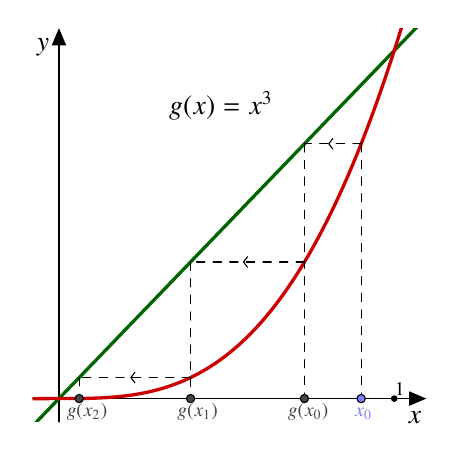
\begin{tikzpicture}[line cap=round,line join=round,>=triangle 45,x=4.258348923866512cm,y=4.41985639199633cm]
\draw[->,color=black] (-0.07868,0.) -- (1.095483998627919,0.);
%\foreach \x in {,0.2,0.4,0.6,0.8,1.}
%\draw[shift={(\x,0)},color=black] (0pt,-2pt);
\draw[color=black] (1.06,-0.1) node [anchor=south] {$x$};
\draw[->,color=black] (0.,-0.06709600189464562) -- (0.,1.0641624727142172);
%\foreach \y in {,0.2,0.4,0.6,0.8,1.}
%\draw[shift={(0,\y)},color=black] (2pt,0pt) -- (-2pt,0pt);
\draw[color=black] (0,1.01) node [anchor=east] {$y$};
\clip(-0.07868,-0.06709600189464562) rectangle (1.095483998627919,1.0641624727142172);
\draw[line width=1.2pt,color=qqwuqq,smooth,samples=100,domain=-0.07868:1.095483998627919] plot(\x,{(\x)});
\draw[line width=1.2pt,color=ccqqqq,smooth,samples=100,domain=-0.07868:1.095483998627919] plot(\x,{(\x)^(3.0)});
\draw [dash pattern=on 3pt off 3pt] (0.9012959396283815,0.7321536700141503)-- (0.9012959396283815,0.);
\draw [dash pattern=on 3pt off 3pt] (0.7321536700141503,0.7321536700141503)-- (0.7321536700141503,0.);
\draw [dash pattern=on 3pt off 3pt] (0.9012959396283815,0.7321536700141503)-- (0.7321536700141503,0.7321536700141503);
\draw [dash pattern=on 3pt off 3pt] (0.8048702644505034,0.7321536700141503) -- (0.816724804821266,0.7473951764085811);
\draw [dash pattern=on 3pt off 3pt] (0.8048702644505034,0.7321536700141503) -- (0.816724804821266,0.7169121636197195);
\draw [dash pattern=on 3pt off 3pt] (0.7321536700141503,0.39247024010599835)-- (0.39247024010599835,0.39247024010599835);
\draw [dash pattern=on 3pt off 3pt] (0.5504574146893118,0.3924702401059984) -- (0.5623119550600744,0.4077117465004292);
\draw [dash pattern=on 3pt off 3pt] (0.5504574146893118,0.3924702401059984) -- (0.5623119550600744,0.3772287337115676);
\draw [dash pattern=on 3pt off 3pt] (0.39247024010599835,0.39247024010599835)-- (0.39247024010599835,0.);
\draw [dash pattern=on 3pt off 3pt] (0.39247024010599835,0.06045332507481716)-- (0.06045332507481716,0.06045332507481716);
\draw [dash pattern=on 3pt off 3pt] (0.21460724221964514,0.06045332507481713) -- (0.22646178259040778,0.07569483146924792);
\draw [dash pattern=on 3pt off 3pt] (0.21460724221964514,0.06045332507481713) -- (0.22646178259040778,0.045211818680386345);
\draw [dash pattern=on 3pt off 3pt] (0.06045332507481716,0.06045332507481716)-- (0.06045332507481716,0.);
\draw (0.48356391472759974,0.8406203789292322) node[anchor=center] {$g(x)=x^3$};
\begin{scriptsize}
\draw [fill=black] (1.,0.) circle (1.0pt);
\draw[color=black] (1.0164537294895013,0.027740037892923702) node {1};
\draw [fill=xdxdff] (0.9012959396283815,0.) circle (1.5pt);
\draw[color=xdxdff] (0.9080693603853858,-0.045) node {$x_0$};
\draw [fill=uuuuuu] (0.7321536700141503,0.) circle (1.5pt);
\draw[color=uuuuuu] (0.7432347990395433,-0.04) node {$g(x_0)$};
\draw [fill=uuuuuu] (0.39247024010599835,0.) circle (1.5pt);
\draw[color=uuuuuu] (0.4135656763478584,-0.04) node {$g(x_1)$};
\draw [fill=uuuuuu] (0.06045332507481716,0.) circle (1.5pt);
\draw[color=uuuuuu] (0.08360651520782803,-0.04) node {$g(x_2)$};
\end{scriptsize}
\end{tikzpicture}
    \caption{�� \ref{Ex:1.20}.}
  \end{figure}
\end{Exa}

\begin{Exa}\label{Ex:1.21}
  \begin{equation*}
    g(x) = 2 x - x^2,\ x' = g(x) = 2 x - x^2.
  \end{equation*}
  0 ���ų��, 1 ��������. $x = 1$ ȡ�����ֵ.
  \begin{figure}[!ht]
    \centering
    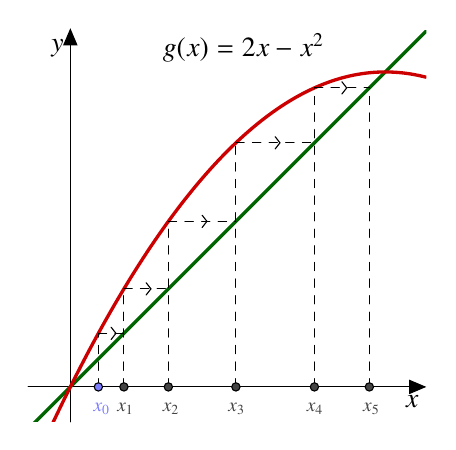
\begin{tikzpicture}[line cap=round,line join=round,>=triangle 45,x=4.0cm,y=4.0cm]
\draw[->,color=black] (-0.13368408198645645,0.) -- (1.1302167706402606,0.);
%\foreach \x in {,1.}
%\draw[shift={(\x,0)},color=black] (0pt,2pt) -- (0pt,-2pt) node[below] {\footnotesize $\x$};
\draw[color=black] (1.0839412245486646,0.005) node [below] {$x$};
\draw[->,color=black] (0.,-0.11061734584836362) -- (0.,1.1388223986247286);
%\foreach \y in {,1.}
%\draw[shift={(0,\y)},color=black] (2pt,0pt) -- (-2pt,0pt) node[left] {\footnotesize $\y$};
\draw[color=black] (0.01,1.075193522748784) node [left] {$y$};
%\draw[color=black] (0pt,-10pt) node[right] {\footnotesize $0$};
\clip(-0.13368408198645645,-0.11061734584836362) rectangle (1.1302167706402606,1.1388223986247286);
\draw[line width=1.2pt,color=qqwuqq,smooth,samples=100,domain=-0.13368408198645645:1.1302167706402606] plot(\x,{(\x)});
\draw[line width=1.2pt,color=ccqqqq,smooth,samples=100,domain=-0.13368408198645645:1.1302167706402606] plot(\x,{2.0*(\x)-(\x)^(2.0)});
\draw [dash pattern=on 3pt off 3pt] (0.0890169835793495,0.)-- (0.0890169835793495,0.17010994379313282);
\draw [dash pattern=on 3pt off 3pt] (0.0890169835793495,0.17010994379313282)-- (0.17010994379313282,0.17010994379313282);
\draw [dash pattern=on 3pt off 3pt] (0.14474762724754614,0.1701099437931328) -- (0.1295634636862412,0.1505874477857407);
\draw [dash pattern=on 3pt off 3pt] (0.14474762724754614,0.1701099437931328) -- (0.1295634636862412,0.18963243980052485);
\draw [dash pattern=on 3pt off 3pt] (0.17010994379313282,0.)-- (0.17010994379313282,0.31128249460896285);
\draw [dash pattern=on 3pt off 3pt] (0.17010994379313282,0.31128249460896285)-- (0.31128249460896285,0.31128249460896285);
\draw [dash pattern=on 3pt off 3pt] (0.25588038276235275,0.31128249460896285) -- (0.24069621920104783,0.29175999860157076);
\draw [dash pattern=on 3pt off 3pt] (0.25588038276235275,0.31128249460896285) -- (0.24069621920104783,0.3308049906163549);
\draw [dash pattern=on 3pt off 3pt] (0.31128249460896285,0.)-- (0.31128249460896285,0.5256681977679467);
\draw [dash pattern=on 3pt off 3pt] (0.31128249460896285,0.5256681977679467)-- (0.5256681977679467,0.5256681977679467);
\draw [dash pattern=on 3pt off 3pt] (0.4336595097497597,0.5256681977679467) -- (0.4184753461884547,0.5061457017605547);
\draw [dash pattern=on 3pt off 3pt] (0.4336595097497597,0.5256681977679467) -- (0.4184753461884547,0.5451906937753388);
\draw [dash pattern=on 3pt off 3pt] (0.5256681977679467,0.)-- (0.5256681977679467,0.7750093413912923);
\draw [dash pattern=on 3pt off 3pt] (0.5256681977679467,0.7750093413912923)-- (0.7750093413912923,0.7750093413912923);
\draw [dash pattern=on 3pt off 3pt] (0.6655229331409243,0.7750093413912924) -- (0.6503387695796193,0.7554868453839003);
\draw [dash pattern=on 3pt off 3pt] (0.6655229331409243,0.7750093413912924) -- (0.6503387695796193,0.7945318373986844);
\draw [dash pattern=on 3pt off 3pt] (0.7750093413912923,0.)-- (0.7750093413912923,0.94937920353882);
\draw [dash pattern=on 3pt off 3pt] (0.7750093413912923,0.94937920353882)-- (0.94937920353882,0.94937920353882);
\draw [dash pattern=on 3pt off 3pt] (0.8773784360263611,0.94937920353882) -- (0.8621942724650562,0.929856707531428);
\draw [dash pattern=on 3pt off 3pt] (0.8773784360263611,0.94937920353882) -- (0.8621942724650562,0.9689016995462121);
\draw [dash pattern=on 3pt off 3pt] (0.94937920353882,0.)-- (0.94937920353882,0.94937920353882);
\draw (0.55,1.075193522748784) node {$g(x) = 2 x - x^2$};
\begin{scriptsize}
\draw [fill=xdxdff] (0.0890169835793495,0.) circle (1.5pt);
\draw[color=xdxdff] (0.09913975928688615,-0.07012624301821711) node {$x_0$};
\draw [fill=uuuuuu] (0.17010994379313282,0.) circle (1.5pt);
\draw[color=uuuuuu] (0.17433752168572975,-0.07012624301821711) node {$x_1$};
\draw [fill=uuuuuu] (0.31128249460896285,0.) circle (1.5pt);
\draw[color=uuuuuu] (0.31894860322196733,-0.07012624301821711) node {$x_2$};
\draw [fill=uuuuuu] (0.5256681977679467,0.) circle (1.5pt);
\draw[color=uuuuuu] (0.5271885606341495,-0.07012624301821711) node {$x_3$};
\draw [fill=uuuuuu] (0.7750093413912923,0.) circle (1.5pt);
\draw[color=uuuuuu] (0.7759196208764784,-0.07012624301821711) node {$x_4$};
\draw [fill=uuuuuu] (0.94937920353882,0.) circle (1.5pt);
\draw[color=uuuuuu] (0.955237361981413,-0.07012624301821711) node {$x_5$};
\end{scriptsize}
\end{tikzpicture}
    \caption{�� \ref{Ex:1.21}.}
  \end{figure}
\end{Exa}

\paragraph{�ȶ���}\

�����ȶ� $\Leftrightarrow$ �����еĽ����� $x^*$.

\begin{Def}\
  \begin{enumerate}
    \item $x^*$ �ȶ�: ��ֵ��С����, ����ܲ���������. ��ͼ \ref{Fi:1.24}.

    $\forall U$, $\exists V$, s.t. $\forall n$, $g^n(V) \subset U$.

    \begin{figure}[!ht]
      \centering
      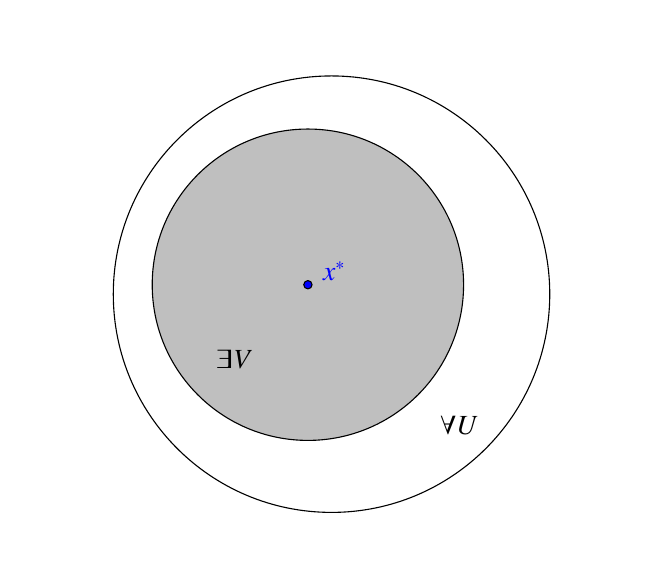
\begin{tikzpicture}[line cap=round,line join=round,>=triangle 45,x=1.0cm,y=1.0cm]
\clip(-3.6788732394366295,-1.5084507042253508) rectangle (3.9281690140845087,5.184507042253532);
\draw [fill=black,fill opacity=0.25] (-0.12,1.92) circle (1.977169694285243cm);
\draw(0.18,1.8) circle (2.771569952211201cm);
\draw (-1.4014084507042315,1.2183098591549348) node[anchor=north west] {$\exists V$};
\draw (1.4338028169014063,0.38169014084507435) node[anchor=north west] {$\forall U$};
\draw [fill=qqqqff] (-0.12,1.92) circle (1.5pt);
\draw[color=qqqqff] (0.2098591549295736,2.0936619718309926) node {$x^*$};
\end{tikzpicture}
      \caption{$\forall x \in V \Rightarrow g^n(x) \in U$}\label{Fi:1.24}
    \end{figure}

    \item $x^*$ ���� (�ֲ�). ��ͼ \ref{Fi:1.25}.

    $\exists V$ s.t. $x \in V \Rightarrow \lim \limits_{n \to \infty} g^n(x) = x^*$.

    \begin{figure}[!ht]
      \centering
      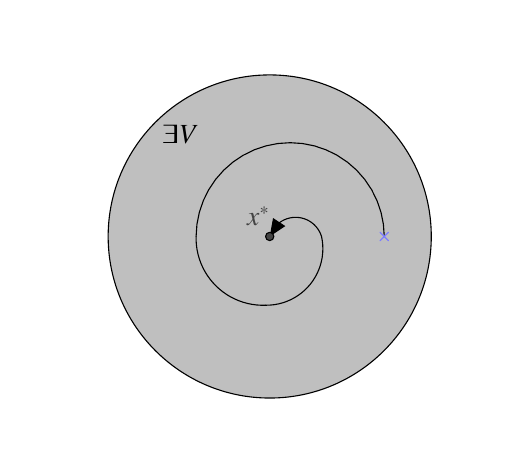
\begin{tikzpicture}[line cap=round,line join=round,>=triangle 45,x=0.5129618685123939cm,y=0.5129618685123939cm]
\clip(-5.992572399906515,-4.577798046271045) rectangle (5.766471307248279,5.169515169232014);
\draw [fill=black,fill opacity=0.25] (0.,0.) circle (2.0518474740495756cm);
\draw [shift={(0.5065664609490944,-0.007478511587597047)}] plot[domain=0.0032108039566619466:3.1383818496331313,variable=\t]({1.*2.3291750409587015*cos(\t r)+0.*2.3291750409587015*sin(\t r)},{0.*2.3291750409587015*cos(\t r)+1.*2.3291750409587015*sin(\t r)});
\draw [shift={(-0.16339949395041392,-0.04380229462495752)}] plot[domain=3.115199090406624:4.752229535452507,variable=\t]({1.*1.6597751629060287*cos(\t r)+0.*1.6597751629060287*sin(\t r)},{0.*1.6597751629060287*cos(\t r)+1.*1.6597751629060287*sin(\t r)});
\draw [shift={(-0.084568837503857,-0.30187307261879415)}] plot[domain=-1.579880552776677:0.2172602517466106,variable=\t]({1.*1.400445087801699*cos(\t r)+0.*1.400445087801699*sin(\t r)},{0.*1.400445087801699*cos(\t r)+1.*1.400445087801699*sin(\t r)});
\draw [shift={(0.6414770696297287,-0.1969466703907538)}] plot[domain=0.2978851954471936:2.8437074581425996,variable=\t]({1.*0.6710296728452089*cos(\t r)+0.*0.6710296728452089*sin(\t r)},{0.*0.6710296728452089*cos(\t r)+1.*0.6710296728452089*sin(\t r)});
\draw [->] (0.02230923913889944,0.034) -- (0.,0.);
\draw (-2.9,3.0) node[anchor=north west] {$\exists V$};
\draw [fill=uuuuuu] (0.,0.) circle (1.5pt);
\draw[color=uuuuuu] (-0.29266934022659397,0.5) node {$x^*$};
\draw [color=xdxdff] (2.8357294958801833,0.)-- ++(-1.5pt,-1.5pt) -- ++(3.0pt,3.0pt) ++(-3.0pt,0) -- ++(3.0pt,-3.0pt);
\end{tikzpicture}
      \caption{$\forall x \in V \Rightarrow \lim \limits_{n \to \infty} g^n(x) = x^*$.}\label{Fi:1.25}
    \end{figure}

    \item $\text{�����ȶ�} = \text{�ȶ�} + \text{����}$.

    \item ���ȶ� $\Leftrightarrow$ �����ȶ���.
  \end{enumerate}
\end{Def}

\begin{Thm}[һά���]
  \begin{equation*}
    \dot{x} = g(x),\ (g \in C^1),\ |g'(x^*)| < 1,
  \end{equation*}
  $\Rightarrow \exists V$, $\forall x \in V$, $\lim\limits_{n \to \infty} g^n(x) = x^*$.
\end{Thm}
\begin{proof}
  $\because g\in C^1$, $|g'(x^*)| < 1$, �� $V = (x^* - \epsilon, x^* + \epsilon)$,

  $\Rightarrow \exists A < 1$, ʹ�� $|g'(x)| < A < 1$, ($x \in V$).

  ��ֵ����
  \begin{align*}
    |g(x) - x^*| & = |g(x) - g(x^*)|,\\
    & = |g'(\delta) (x - x^*)|,\ (\delta \in V),\\
    & \leq A |x - x^*|,\\
    & < |x - x^*| < \epsilon.
  \end{align*}

  $\Rightarrow |g^n(x) - x^*| \leq A^n |x - x^*| \to 0$.

  $\therefore \lim\limits_{n \to \infty} g^n(x) = x^*$.
\end{proof}

\begin{Cor}
  \begin{equation*}
    |g'(x^*)| > 1 \Rightarrow \exists V = N(x^*),\ \forall x \in V \setminus \{x^*\},\ \exists n,\ \text{s.t.}\ g^n(x) \notin V.
  \end{equation*}
\end{Cor}

\begin{Exa}
  Ѱ��
  \begin{align*}
    x' & = r x (1 - x),\\
    x' & = x \e^{r (1 - x)},
  \end{align*}
  ���ȶ����� (�ֲ��ȶ�).
\end{Exa}

\begin{Exa}\label{Ex:1.23}
  $g(x) = r x(1 - x),\ r = 3.84$. ����������!
  \begin{figure}[!ht]
    \centering
    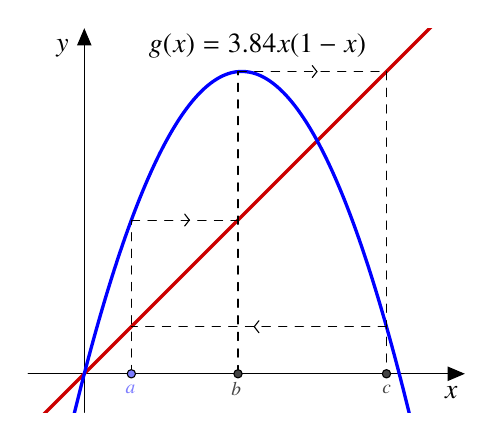
\begin{tikzpicture}[line cap=round,line join=round,>=triangle 45,x=4.0cm,y=4.0cm]
\draw[->,color=black] (-0.17800802090501203,0.) -- (1.208261351669273,0.);
%\foreach \x in {,0.2,0.4,0.6,0.8,1.,1.2}
%\draw[shift={(\x,0)},color=black] (0pt,-2pt);
\draw[color=black] (1.1630876042941436,-0.11) node [anchor=south] {$x$};
\draw[->,color=black] (0.,-0.12256781550598113) -- (0.,1.0971233636225146);
%\foreach \y in {,0.2,0.4,0.6,0.8,1.}
%\draw[shift={(0,\y)},color=black] (2pt,0pt) -- (-2pt,0pt);
\draw[color=black] (-0.12,1.0350094609817115) node [anchor=west] {$y$};
\clip(-0.17800802090501203,-0.12256781550598113) rectangle (1.208261351669273,1.0971233636225146);
\draw[line width=1.2pt,color=ccqqqq,smooth,samples=100,domain=-0.17800802090501203:1.208261351669273] plot(\x,{(\x)});
\draw[line width=1.2pt,color=qqqqff,smooth,samples=100,domain=-0.17800802090501203:1.208261351669273] plot(\x,{3.84*(\x)*(1.0-(\x))});
\draw [dash pattern=on 3pt off 3pt] (0.1494068966,0.)-- (0.1494068966,0.4880043872576905);
\draw [dash pattern=on 3pt off 3pt] (0.1494068966,0.4880043872576905)-- (0.4880043872576905,0.4880043872576905);
\draw [dash pattern=on 3pt off 3pt] (0.33352827778630967,0.4880043872576905) -- (0.31870564192884526,0.46894671258380777);
\draw [dash pattern=on 3pt off 3pt] (0.33352827778630967,0.4880043872576905) -- (0.31870564192884526,0.5070620619315732);
\draw [dash pattern=on 3pt off 3pt] (0.4880043872576905,0.)-- (0.4880043872576905,0.9594474442557563);
\draw [dash pattern=on 3pt off 3pt] (0.4880043872576905,0.9594474442557563)-- (0.9594474442557563,0.9594474442557563);
\draw [dash pattern=on 3pt off 3pt] (0.7385485516141878,0.9594474442557563) -- (0.7237259157567234,0.9403897695818736);
\draw [dash pattern=on 3pt off 3pt] (0.7385485516141878,0.9594474442557563) -- (0.7237259157567234,0.9785051189296391);
\draw [dash pattern=on 3pt off 3pt] (0.9594474442557563,0.9594474442557563)-- (0.9594474442557563,0.);
\draw [dash pattern=on 3pt off 3pt] (0.9594474442557563,0.14940689651271807)-- (0.14940689651271807,0.14940689651271807);
\draw [dash pattern=on 3pt off 3pt] (0.539604534526773,0.14940689651271805) -- (0.5544271703842374,0.1684645711866008);
\draw [dash pattern=on 3pt off 3pt] (0.539604534526773,0.14940689651271805) -- (0.5544271703842374,0.1303492218388353);
\draw (0.55,1.04) node {$g(x)=3.84 x (1-x)$};
\begin{scriptsize}
\draw [fill=xdxdff] (0.1494068966,0.) circle (1.5pt);
\draw[color=xdxdff] (0.14667828835373092,-0.05) node {$a$};
\draw [fill=uuuuuu] (0.4880043872576905,0.) circle (1.5pt);
\draw[color=uuuuuu] (0.48265803445625627,-0.05) node {$b$};
\draw [fill=uuuuuu] (0.9594474442557563,0.) circle (1.5pt);
\draw[color=uuuuuu] (0.9598057411060611,-0.05) node {$c$};
\end{scriptsize}
\end{tikzpicture}
    \caption{�� \ref{Ex:1.23}.}
  \end{figure}
\end{Exa}

1975 ��, Li-Yorke, 3 ���� $\Rightarrow$ Chaos (����), Periole 3 impleis chaos.

1964 ��, Shakovskii, �ڿ���,
\begin{align*}
  &3\prec5\prec7\prec9\prec\cdots\\
  &2\cdot3\prec2\cdot5\prec2\cdot7\prec2\cdot9\prec\cdots\\
  &\cdots\\
  &2^n\cdot3\prec2^n\cdot5\prec2^n\cdot7\prec2^n\cdot9\prec\cdots\\
  &\cdots\\
  &2^n\prec\cdots\prec2^{100}\prec\cdots\prec16\prec8\prec4\prec2\prec1
\end{align*}
$m$ ���� $\Rightarrow n$ ����, �� $m < n$. 

\chapter{ƽ��ϵͳ�����}

��άϵͳ
\begin{equation}\label{Eq:2.1}
  \dot{x} = P(x, y),\ \dot{y} = Q(x, y),
\end{equation}
$P$, $Q \in G$ ������
\begin{inparaenum}[(i)]
  \item ����;
  \item Lipschitz ����.
\end{inparaenum}
�� $(x(t), y(t))$ Ϊƽ����һ����, ƽ��� $(x^*, y^*) \xrightarrow{\text{ƽ��}}$ ԭ��.

Jacobi����
\begin{equation*}
  A =
  \begin{pmatrix}
    a & b \\
    c & d
  \end{pmatrix}
  = \left.J(P, Q)\right|_{(x^*, y^*)}.
\end{equation*}

����ϵͳ
\begin{equation}\label{Eq:2.2}
  \dot{x} = a x + b y, \ \dot{y} = c x + d y.
\end{equation}
\begin{enumerate}
  \item �����Է��� $\rightarrow$ ���Է��� $\Rightarrow$ ���� (��).
  \item ���Է��� $\xrightarrow{\text{��������}}$ �����Է�������.
\end{enumerate}

���ƽ�����˫����, ������ \eqref{Eq:2.2} ��������Ӧ�����Է���ƽ���ֲ����.
\begin{enumerate}
  \item $|A| \neq 0$, ������� (ƽ���).
  \item $|A| = 0$, �߽����.
\end{enumerate}

\begin{Exa}\label{Ex:2.1}
  ���� Lotka-Volterra ϵͳ
  \begin{align*}
    \dot{x}_1 = x_1 (r_1 + a_{11} x_1 + a_{12} x_2),\\
    \dot{x}_2 = x_2 (r_2 + a_{21} x_1 + a_{22} x_2),
  \end{align*}
  ��ƽ��� $(0, 0)$ ����ƽ��� $(x^*, y^*)$, �ֱ��ҳ���Ӧ������ϵͳ.
\end{Exa}

%%%%%%%%%%%%%%%%%%%%%%%%%%%%%%%%%%%%%%%%%%%%%%%%%%
%%%%%%%%%%%%%%%%%%%%%%%%%%%%%%%%%%%%%%%%%%%%%%%%%%
%%%%%%%%%%%%%%%%%%%%%%%%%%%%%%%%%%%%%%%%%%%%%%%%%%
%%%%%%%%%%%%%%%%%%%%%%%%%%%%%%%%%%%%%%%%%%%%%%%%%%
%%%%%%%%%%%%%%%%%%%%%%%%%%%%%%%%%%%%%%%%%%%%%%%%%%

\section{���, �ȶ���}

\subsection{����ϵͳ�����}

\begin{equation}
  \dot{X} = A X, \ A =
  \begin{pmatrix}
    a & b \\
    c & d
  \end{pmatrix}, \ |A| \neq 0.
\end{equation}

\begin{Prop}
  $A$ ����\footnote{����: $X = T Y$, $\dot{X} = A X$, $Y = B Y$}������֮һ:
  \begin{enumerate}
    \item \label{M 1} $\begin{pmatrix}\lambda & 0\\ 0 & \mu\end{pmatrix}$;
    \item \label{M 2} $\begin{pmatrix}\lambda & 0\\ 1 & \lambda\end{pmatrix}$, �� $\lambda = \mu$ ʱ�ľ��� \ref{M 1} ��Ӧ�� Jordan ��׼�Ͳ�ͬ;
    \item \label{M 3} $\begin{pmatrix}\alpha &  - \beta\\ \beta & \alpha\end{pmatrix}$.
  \end{enumerate}
  ���� \ref{M 1} ������ֵΪ $\lambda$, $\mu$. ���� \ref{M 2} ������ֵΪ $\lambda$ (�ظ�).���� \ref{M 3} ������ֵΪ $\alpha \pm i \beta$.
\end{Prop}

\begin{equation}
  \dot{y} = B y,\ y=(y_1, y_2).
\end{equation}

\begin{enumerate}[I.]
  \item $B = \begin{pmatrix}\lambda & 0\\ 0 & \mu\end{pmatrix}$.

  ��
  \begin{align*}
    \dot{y}_1 = \lambda y_1,\\
    \dot{y}_2 = \mu y_2.
  \end{align*}
  ��ֵΪ $(c_1, c_2)$, ��Ϊ $y_1 = c_1 \e^{\lambda t}$, $y_2 = c_2 \e^{\mu t}$.
  \begin{enumerate}[{I}-1]
    \item ����: $\lambda$, $\mu$ ���. $\lambda > 0$, $\mu < 0$, ����˫���� $y^{|\mu|}_1 y^\lambda_2 = c^{|\mu|}_1 c^\lambda_2$.
    \begin{figure}[!ht]
      \centering
      \begin{tikzpicture}[line cap=round,line join=round,>=angle 60,x=2.5cm,y=2.5cm,]%,>=triangle 45
\draw[-{Stealth[scale=1.3]},color=black] (-1.,0.) -- (1.1,0.);
%\foreach \x in {-1.,-0.8,-0.6,-0.4,-0.2,0.2,0.4,0.6,0.8}
%\draw[shift={(\x,0)},color=black] (0pt,-2pt);
\draw[color=black] (1.0,-0.1) node {$y_1$};
\draw[-{Stealth[scale=1.3]},color=black] (0.,-1.) -- (0.,1.1);
%\foreach \y in {-1.,-0.8,-0.6,-0.4,-0.2,0.2,0.4,0.6,0.8}
%\draw[shift={(0,\y)},color=black] (2pt,0pt) -- (-2pt,0pt);
\draw[color=black] (-0.11,1.0) node {$y_2$};
\clip(-1.,-1.) rectangle (1.,1.);
\draw [arrows={-Latex[scale=1.3]},thin] (0.4,0.) -- (0.5,0.);
\draw [arrows={-Latex[scale=1.3]},thin] (-0.4,0.) -- (-0.5,0.);
\draw [arrows={-Latex[scale=1.3]},thin] (0.,1.) -- (0.,0.5);
\draw [arrows={-Latex[scale=1.3]},thin] (0.,-1.) -- (0.,-0.5);
\draw [shift={(0.6384911867426616,0.6384911867426616)}] plot[domain=3.0610349770393195:4.792946656935163,variable=\t]({1.*0.5494095051538909*cos(\t r)+0.*0.5494095051538909*sin(\t r)},{0.*0.5494095051538909*cos(\t r)+1.*0.5494095051538909*sin(\t r)});
\draw [shift={(-0.6384911867426617,0.6384911867426618)}] plot[domain=-1.6513540033453697:0.08055767655047334,variable=\t]({1.*0.549409505153891*cos(\t r)+0.*0.549409505153891*sin(\t r)},{0.*0.549409505153891*cos(\t r)+1.*0.549409505153891*sin(\t r)});
\draw [shift={(-0.6384911867426619,-0.6384911867426618)}] plot[domain=-0.08055767655047319:1.6513540033453697,variable=\t]({1.*0.5494095051538912*cos(\t r)+0.*0.5494095051538912*sin(\t r)},{0.*0.5494095051538912*cos(\t r)+1.*0.5494095051538912*sin(\t r)});
\draw [shift={(0.6384911867426616,-0.6384911867426616)}] plot[domain=1.490238650244423:3.2221503301402667,variable=\t]({1.*0.5494095051538909*cos(\t r)+0.*0.5494095051538909*sin(\t r)},{0.*0.5494095051538909*cos(\t r)+1.*0.5494095051538909*sin(\t r)});
\draw [arrows={-Latex[scale=1.3]},thin] (0.33979818200182577,0.17640618527468596) -- (0.3937370451109275,0.14555018476187234);
\draw [arrows={-Latex[scale=1.3]},thin] (-0.33979818200182577,-0.17640618527468593) -- (-0.3937370451109275,-0.1455501847618723);
\draw [arrows={-Latex[scale=1.3]},thin] (0.33979818200182577,-0.17640618527468596) -- (0.3937370451109275,-0.14555018476187234);
\draw [arrows={-Latex[scale=1.3]},thin] (-0.33979818200182577,0.176406185274686) -- (-0.3937370451109275,0.1455501847618724);
\begin{scriptsize}
\draw [fill=uuuuuu] (0.,0.) circle (1.5pt);
\end{scriptsize}
\end{tikzpicture} 
      \caption{����.}
    \end{figure}

    \item ���: $\lambda \cdot \mu > 0$.

    \begin{itemize}
      \item $\lambda = \mu$.
      \begin{figure}[!ht]
        \centering
        \psfrag{yone}[][]{$y_1$}\psfrag{ytwo}[][]{$y_2$}
        \includegraphics[width = 0.3\textwidth]{T30.eps}
        \caption{$\lambda = \mu$.}
      \end{figure}
      \item $\lambda \neq \mu$. $\lambda > 0$, $\mu > 0$, ���ȶ���� (Դ), $\lambda < 0$, $\mu < 0$, �ȶ���� (Ԩ).
      \begin{figure}[!ht]
        \centering
        \psfrag{yone}[][]{$y_1$}\psfrag{ytwo}[][]{$y_2$}
        \includegraphics[width = 0.3\textwidth]{T31.eps}
        \caption{$\lambda \neq \mu$.}
      \end{figure}
    \end{itemize}
  \end{enumerate}

  \item $B = \begin{pmatrix}\lambda & 0\\ 1 & \lambda\end{pmatrix}, \ \lambda < 0$. $y_1 = c_1 \e^{\lambda t}$, $y_2 = (c_1 t + c_2) \e^{\lambda t}$.
  \begin{enumerate}
    \item $(c_1, c_2) = (0, 1)$, $(0,  - 1)$.
    \begin{figure}[!ht]
      \centering
      \psfrag{yone}[][]{$y_1$}\psfrag{ytwo}[][]{$y_2$}
      \includegraphics[width = 0.3\textwidth]{T32.eps}
      \caption{���� II (a).}
    \end{figure}
    \item $(c_1, c_2) = (1, 0)$, $( - 1, 0)$.
    \begin{figure}[!ht]
      \centering
      \psfrag{yone}[][]{$y_1$}\psfrag{ytwo}[][]{$y_2$}
      \includegraphics[width = 0.3\textwidth]{T33.eps}
      \caption{���� II (b).}
    \end{figure}
  \end{enumerate}

  \item $B = \begin{pmatrix}\alpha &  - \beta \\ \beta & \alpha\end{pmatrix}$. �任 $x = r \cos \theta$, $y = r \sin \theta \Rightarrow r = c_1 \e^{\alpha t}$, $\theta = \beta t + c_2$.
  \begin{enumerate}[{III}-1]
    \item ���� (���ȶ�): $\alpha > 0$, $\beta > 0$.
    \begin{figure}[!htb]
      \centering
      \psfrag{O}{$O$}
      \includegraphics[width = 0.3\textwidth]{T34.eps}
      \caption{���ȶ�����}
    \end{figure}
    \item ���� (�ȶ�): $\alpha < 0$, $\beta < 0$. ������������!
    \begin{figure}[!htb]
      \centering
      \psfrag{O}{$O$}
      \includegraphics[width = 0.3\textwidth]{T35.eps}
      \caption{�ȶ�����}
    \end{figure}
    \item ����: $\alpha = 0$, $r = c_1$, $\theta = \beta t + c_2$. (�ر�)
    \begin{figure}[!htb]
      \centering
      \psfrag{O}{$O$}
      \includegraphics[width = 0.3\textwidth]{T36.eps}
      \caption{���������}
    \end{figure}
  \end{enumerate}
\end{enumerate}

�ܽ�: $A = \begin{pmatrix} a & b \\ c & d\end{pmatrix}$, $|A| \neq 0$, ����ֵ $\lambda_1$, $\lambda_2$:
\begin{enumerate}[i]
  \item \label{Q 1} $\Rer \lambda_1$, $\Rer \lambda_2 < 0$, �ȶ��Ľ������;
        $\Rer \lambda_1$, $\Rer \lambda_2 > 0$, ���ȶ��Ľ������.
  \item \label{Q 2} $\Rer \lambda_1 \cdot\Rer \lambda_2 < 0$, ����. ��ʱ, $\Rer \lambda_i = \lambda_i$.
  \item \label{Q 3} $\Rer \lambda_1 = \Rer \lambda_2 = 0$, ����.
\end{enumerate}
������� \ref{Q 1} �� \ref{Q 2} ��Ϊ˫����, \ref{Q 3} ��Ϊ��˫����. $|A| = 0$, ��� $=$ ����, ��������ͳ.

һ�����Գ�΢�ַ��̽�Ϊ:
\begin{equation}
  c_1 \e^{\Rer \lambda_1 t} P(\cos t, \sin t) Q(t) + c_2 \e^{\Rer \lambda_2 t}\bigtriangleup
\end{equation}

������� \ref{Q 1}.
\begin{figure}[!htb]
  \centering
  \subfloat[���]{\psfrag{yone}[][]{$y_1$}\psfrag{ytwo}[][]{$y_2$}\includegraphics[width = 0.25\textwidth]{T37.eps}}\hspace{30pt}
  \subfloat[����]{\psfrag{yone}[][]{$y_1$}\psfrag{ytwo}[][]{$y_2$}\includegraphics[width = 0.25\textwidth]{T38.eps}}
  \caption{���� \ref{Q 1}.}
\end{figure}

%\setcounter{totalnumber}{5}

������� \ref{Q 2}.
\begin{figure}[!ht]
  \centering
  \psfrag{yone}[][]{$y_1$}\psfrag{ytwo}[][]{$y_2$}
  \psfrag{yws}[br][br]{$\text{һά�ȶ�����}$}\psfrag{ybs}[bl][bl]{$\text{һά���ȶ�����}$}
  \includegraphics[width = 0.25\textwidth]{T39.eps}
  \caption{����}
\end{figure}

������� \ref{Q 3}.
\begin{figure}[!ht]
  \centering
  \psfrag{yone}[][]{$y_1$}\psfrag{ytwo}[][]{$y_2$}
  \includegraphics[width = 0.25\textwidth]{T40.eps}
  \caption{����}
\end{figure}

\begin{Exa}
  ���� Lotka-Volterra ϵͳ (�� \ref{Ex:2.1}) ��ƽ��� $(x^*_1, x^*_2)$ ������ϵͳ�ȶ������ȶ������㡢���ĵ�����.
\end{Exa}

%%%%%%%%%%%%%%%%%%%%%%%%%%%%%%%%%%%%%%%%%%%%%%%%%%
%%%%%%%%%%%%%%%%%%%%%%%%%%%%%%%%%%%%%%%%%%%%%%%%%%
%%%%%%%%%%%%%%%%%%%%%%%%%%%%%%%%%%%%%%%%%%%%%%%%%%
%%%%%%%%%%%%%%%%%%%%%%%%%%%%%%%%%%%%%%%%%%%%%%%%%%
%%%%%%%%%%%%%%%%%%%%%%%%%%%%%%%%%%%%%%%%%%%%%%%%%%

\section{���������}

\begin{Def}
  ���ij����û��������� $\Rightarrow$ �������.
\end{Def}

��ά������ϵͳ
\begin{equation}\label{Eq:2.6}
  \begin{aligned}
    \dot{x} & = a x + b y + \Phi(x, y),\\
    \dot{y} & = c x + d y + \Psi(x, y).
  \end{aligned}
\end{equation}
���Ӧ����ϵͳΪ
\begin{equation}\label{Eq:2.7}
  \begin{aligned}
    \dot{x} = a x + b y,\\
    \dot{y} = c x + d y.
  \end{aligned}
\end{equation}
������ $\Phi(0, 0) = \Psi(0, 0) = 0$ ��, $(0, 0)$ �Ƿ����� \eqref{Eq:2.6} �� \eqref{Eq:2.7} �����.

\begin{Def}[��ά]
  $\begin{pmatrix}
    a & b\\
    c & d
  \end{pmatrix}$
  ������ֵ�� $\lambda_1$, $\lambda_2$,
  \begin{enumerate}
    \item $\Rer \lambda_i \neq 0 \Rightarrow$ ˫�����, ��: ���㡢���㡢���;
    \item $\Rer \lambda_i = 0 \Rightarrow$ ��˫�����, ��: ����.
  \end{enumerate}
\end{Def}

һ�� $\dot{x} = f(x)$, $A = \diff f(0)$, $x =  A x$.
\begin{Def}[$n$ ά]
  $\lambda_i$ Ϊ$A$ ������ֵ ($i = 1, \dots, n$),
  \begin{enumerate}
    \item $\forall \Rer \lambda_i \neq 0 \Rightarrow$ ˫�����;
    \item $\exists \Rer \lambda_i = 0 \Rightarrow$ ��˫�����.
  \end{enumerate}
  �ر��,
  \begin{enumerate}
    \item $\forall \Rer \lambda_i > 0 \Leftrightarrow 0$ ΪԴ;
    \item $\forall \Rer \lambda_i < 0 \Leftrightarrow 0$ ΪԨ.
  \end{enumerate}
\end{Def}

\begin{Thm}[Hartmon]
  ˫����������������������ϵͳͬ�� (��������һһӳ��). (����������ͬ)
\end{Thm}
\begin{figure}[!ht]
  \centering
  \subfloat[����ϵͳ]{\psfrag{yone}[][]{$y_1$}\psfrag{ytwo}[][]{$y_2$}\includegraphics[width = 0.2\textwidth]{T41.eps}}\hspace{30pt}
  \subfloat[������ϵͳ]{\psfrag{yone}[][]{$y_1$}\psfrag{ytwo}[][]{$y_2$}\includegraphics[width = 0.2\textwidth]{T42.eps}}
  \caption{˫���������ϵͳ�������ϵͳͬ��.}
\end{figure}

\begin{Note}
  ���� $\dot{x} = f(x)$, ������ϵͳΪ $\dot{x} = A x$, ԭ��Ϊ����ϵͳ����, �����ڷ�����ϵͳ, ԭ���Ϊ���� (�ȶ����ȶ�) ������.
\begin{figure}[!ht]
  \centering
  \subfloat[����ϵͳ����]{\psfrag{yone}[][]{$y_1$}\psfrag{ytwo}[][]{$y_2$}\includegraphics[width = 0.2\textwidth]{T40.eps}}\hfill
  \subfloat[������ϵͳ��Ӧ���]{\psfrag{yone}[][]{$y_1$}\psfrag{ytwo}[][]{$y_2$}\includegraphics[width = 0.2\textwidth]{T40.eps}\hspace{2pt}\includegraphics[width = 0.2\textwidth]{T43.eps}\hspace{2pt}\includegraphics[width = 0.2\textwidth]{T44.eps}}
  \caption{ԭ������ϵͳΪ����, ԭϵͳԭ�㲻һ��Ϊ����.}
\end{figure}
\end{Note}

%%%%%%%%%%%%%%%%%%%%%%%%%%%%%%%%%%%%%%%%%%%%%%%%%%
%%%%%%%%%%%%%%%%%%%%%%%%%%%%%%%%%%%%%%%%%%%%%%%%%%
%%%%%%%%%%%%%%%%%%%%%%%%%%%%%%%%%%%%%%%%%%%%%%%%%%
%%%%%%%%%%%%%%%%%%%%%%%%%%%%%%%%%%%%%%%%%%%%%%%%%%
%%%%%%%%%%%%%%%%%%%%%%%%%%%%%%%%%%%%%%%%%%%%%%%%%%

\section{�ȶ���}

\begin{Def}\label{De:2.4}\
  \begin{enumerate}
    \item \label{De:2.4.1} $\forall U \ni x^*$, $\exists V \subset U$, $x^* \in V$ ʹ�õ� $x^0 \in V \Rightarrow x(t) \in U$.

        $\Rightarrow x^*$ (�ֲ�) �ȶ�, �����Ϊ���ȶ�.
    \begin{figure}[!ht]
      \centering
      \psfrag{forallU}{$\forall U$}
      \psfrag{existsV}{$\exists V$}
      \psfrag{x}{$x^*$}
      \psfrag{z}{$x^0$}
      \includegraphics[width = 0.3\textwidth]{T45.eps}
      \caption{�ֲ��ȶ�.}
    \end{figure}
        �ر��, �� $U = V$ ʱ, $\forall U$, $\forall x^0 \in U \Rightarrow x(t) \in U$.

    \item \label{De:2.4.2} $\exists W \Rightarrow x^*$, $\forall x^0 \in \bar{W}$, $\lim \limits_{t \to \infty} x(t) = x^*$.

        $\Rightarrow x^*$ (�ֲ�) ����.

    \item \label{De:2.4.3} �ȶ� $\oplus$ ���� $\Rightarrow$ �����ȶ�.
  \end{enumerate}
\end{Def}

����: �ȶ��Ƿ��̺�����?

���� \ref{De:2.4.1} $\nRightarrow$ \ref{De:2.4.2}, ��Ϊ�������ȶ��ĵ�����������.

���� \ref{De:2.4.2} $\nRightarrow$ \ref{De:2.4.1}, ��ͼ
\begin{figure}[!ht]
  \centering
  \psfrag{S}{$x^*$}
  \psfrag{U}{$U$}
  \includegraphics[width = 0.3\textwidth]{T46.eps}
  \caption{��������, �������ȶ������. ������ʮ������ʮ���.}
\end{figure}

���ڶ�ά������ϵͳ
\begin{equation*}
  \begin{array}{|c|l}
    \cline{1-1}
    \dot{x} = a x + b y & {} + \Phi(x, y),\\
    \dot{y} = c x + d y & {}+ \Psi(x, y).\\
    \cline{1-1}
  \end{array}
\end{equation*}
�ּ�����ϵ������
$A = \begin{pmatrix}
  a & b\\
  c & d
\end{pmatrix}$ ������ֵΪ $\Rer \lambda_i \neq 0$.

\begin{Thm}
  $|A| \neq 0$,
  \begin{enumerate}
    \item $\Rer \lambda_{1, 2} < 0 \Rightarrow$ ������ \eqref{Eq:2.6} ��ԭ�㽥���ȶ�;
    \item $\exists \Rer \lambda_i > 0 \Rightarrow$ ������ \eqref{Eq:2.6} ��ԭ���Dz��ȶ���.
  \end{enumerate}
\end{Thm}

����һ���ƽ��ϵͳ
\begin{equation} \label{Eq:2.8}
  \begin{aligned}
    \dot{x} & = P(x, y),\\
    \dot{y} & = Q(x, y).
  \end{aligned}
\end{equation}
�� Lyapunov �ȶ�������. (1885 ��, ��ʿ����, �ø������� $\Rightarrow$ �ȶ���, LaSalle �� 1960 �꽫 Lyapunov �����ƹ�, �� LaSalle ������ԭ��.)

���ڵ���������:
\begin{enumerate}
  \item Lyapunov (�ֲ��ȶ�������);
  \item ƽ��ϵͳ (˫����) �ȶ����ж�;
  \item ���Ľ���������ж� (���).
\end{enumerate}

\subsection{Lyapunov (Liapunov) �ȶ��Զ���}

\begin{Def}
  $V(x)$ ($V(0) = 0$) ��ԭ������ ($N = N(0) \setminus \{0\}$):
  \begin{enumerate}[(i)]
    \item ����: $V(x) > 0$, $x \in N$;
    \item ����: $V(x) < 0$, $x \in N$;
    \item ������: $V(x) \geq 0$, $x \in N$;
    \item �븺��: $V(x) \leq 0$, $x \in N$.
  \end{enumerate}
\end{Def}

\begin{Thm}[Lyapunov, �̲�����2.5]
  ������ \eqref{Eq:2.8} ���ں��� $V(x, y)$, ʹ��
  \begin{equation*}
    V(0, 0) = 0,
  \end{equation*}
  ��:
  \begin{enumerate}[(i)]
    \item \label{Lyapunov_C1} $V(x, y)$ �� $(0, 0)$ ��������;
    \item \label{Lyapunov_C2} $\dot{V}(x, y)$ �� $(0, 0)$ ���򸺶�,
  \end{enumerate}
  �� $(0, 0)$ ���ǽ����ȶ���.
\end{Thm}

����:
\begin{enumerate}[(i)]
  \item $V(x, y)$ ����, ��ͼ \ref{T 4}.
  \begin{figure}[!ht]
    \centering
    \psfrag{V}{$V$}
    \psfrag{yone}{$x$}
    \psfrag{ytwo}{$y$}
    \includegraphics[width = 0.25\textwidth]{T47.eps}
    \caption{$V(x, y)$ ����ʾ��ͼ.}
    \label{T 4}
  \end{figure}

  $V(x, y) = c$, $c$ ���Сʱ, ����ͼ���DZ�����, ��ͼ \ref{T 5}.
  \begin{figure}[!ht]
    \centering
    \psfrag{yone}{$x$}
    \psfrag{ytwo}{$y$}
    \includegraphics[width = 0.25\textwidth]{T48.eps}
    \caption{����ʾ��ͼ.}
    \label{T 5}
  \end{figure}

  \item $\dot{V}(x, y)$ �����Ķ��弰����.

  �� $(x(t), y(t))$ ��, ���� $V(x, y)$ ��,
  \begin{align*}
    \dot{V}(x, y) & = \frac{\D(V(x(t), y(t)))}{\D t}\\
    & = V_x \cdot \dot{x} + V_y \cdot \dot{y}\\
    & = V_x \cdot P(x, y) + V_y \cdot Q(x, y) < 0,
  \end{align*}
  $\Rightarrow V(x(t), y(t))$ ���� $t$ �ϸ񵥵��ݼ�,

  $\Rightarrow V(x(0), y(0)) = c_1$, $V(x(t), y(t)) = c_2$, $t > 0$,

  $\Rightarrow c_2 < c_1$.
\end{enumerate}
�������� (\ref{Lyapunov_C1}) �� (\ref{Lyapunov_C2}), ��ʾ��ͼ \ref{T 6}.
\begin{figure}[!ht]
  \centering
  \psfrag{yone}{$x$}
  \psfrag{ytwo}{$y$}
  \psfrag{Cone}{$c_1$}
  \psfrag{Ctwo}{$c_2$}
  \includegraphics[width = 0.25\textwidth]{T49.eps}
  \caption{Lyapunov ����ʾ��ͼ.}
  \label{T 6}
\end{figure}

\begin{proof}\
  \begin{enumerate}[1)]
    \item  �ȶ���.

    �� $V$ �� $N$ ������,
    \begin{enumerate}
      \item �� $N$ �� \CJKunderline{��ȡ $\varepsilon$ ��}
        \begin{equation*}
          B_\varepsilon = \{(x, y) \mid x^2 + y^2 \leq \varepsilon^2\}.
        \end{equation*}

      \item ��$m = \min \limits_{x^2 + y^2 = \varepsilon^2} V(x, y) > 0$.

      \item �� $l < m$, ���� $\delta > 0$, �� $x^2 + y^2 < \delta$ ʱ,
        \begin{equation*}
          V(x, y) < l \ (\because V(0, 0) = 0).
        \end{equation*}
        ��ͼ \ref{T 7}.
      \begin{figure}[!ht]
        \centering
        \psfrag{V}{$V$}
        \psfrag{yone}{$x$}
        \psfrag{ytwo}{$y$}
        \psfrag{epsilon}{$\varepsilon$}
        \psfrag{delta}{$\delta$}
        \includegraphics{T50.eps}
        \caption{$l < m$.}
        \label{T 7}
      \end{figure}

      \item $\because$ �� $N$ �� $\dot{V}(x, y) < 0$,

        \CJKunderline{$\Rightarrow$ �� $x^2_0 + y^2_0 < \delta^2$,}

        $\Rightarrow V(x(t), y(t)) < V(x_0, y_0) < l < m$,

        \CJKunderline{$\Rightarrow x^2(t) + y^2(t) < \varepsilon^2$.} �ȶ�!
    \end{enumerate}

    \item  ������.

    $\forall M > 0$ ���ȶ���, ���� $\delta > 0$, �� $x^2_0 + y^2_0 < \delta^2$ ʱ,
    \begin{equation}\label{Eq:2.9}
      \|(x(t), y(t))\|\leq M.
    \end{equation}
    ����, $t \to + \infty$, $V(x(t), y(t)) \to c > 0$, �����ݼ��м���, ��������,
    \begin{equation}\label{Eq:2.10}
      \Rightarrow \exists m > 0, \ \exists t > t_0, \ \|(x(t), y(t))\| \geq m.
    \end{equation}
    �� $h$ ($< 0$) Ϊ $\dot{V}(x, y)$ �� \eqref{Eq:2.9} $\oplus$ \eqref{Eq:2.10} �����е����ֵ, �� $t > t_0$ ʱ:
    \begin{equation*}
      V(x(t), y(t)) - V(x_0, y_0) = \int^t_{t_0} \frac{\D V}{\D t} \D t \leq h(t - t_0).
    \end{equation*}
    $t \to \infty$ ʱ, ����ʽ�ó��� $\leq - \infty$, ì�ܣ�

    $\therefore V(x(t), y(t)) \to 0$.
  \end{enumerate}
\end{proof}

\begin{Note}
  1885 ��, Lyapunov $\to$ 1960 ��, LaSalle. \footnotemark
\end{Note}

\footnotetext{���:

LaSalle J P. ����ϵͳ���ȶ���[M]. �ɶ�: �Ĵ���ѧ����������, 2002.

Hofbauer J, Sigmund K. �����Բ�����Ⱥ����ѧ[M]. �ɶ�: �Ĵ���ѧ����������, 2002.}

\begin{Note}\label{No:2.3}
  1950 ��, $V$ ����� $\Rightarrow$ ȫ�� (����) �ȶ�: �ֲ��ȶ� $\oplus$ ȫ������.

  \begin{inparaenum}
    \item $V$����;
    \item $\dot{V}$����;
    \item $V$�����.
  \end{inparaenum}
  \begin{equation*}
    V(\xi), \ \xi\in G, \ \xi\to\partial G, \ V\to  + \infty.
  \end{equation*}
  ���� $\forall c$, $V(x, y) = c$ �Ľ��涼�DZ�����.
  \begin{figure}[!ht]
    \centering
    \psfrag{v}{$V(x, y) = c$}
    \psfrag{x}{$x^*$}
    \includegraphics[width = 0.25\textwidth]{T51}
    \caption{ע \ref{No:2.3}.}
  \end{figure}
\end{Note}

\begin{Note}
  $V$ ��������������¿ɹ������.
\end{Note}

\begin{Note}
  $\dot{x} = y$, $\dot{y} = - x - y$, ������Ϊ $\frac{ - 1 \pm \sqrt{3}i}{2}$.
  \begin{enumerate}
    \item ���Է��� $\Rightarrow$ ����ȶ���;
    \item \begin{align*}
      V_1 & = x^2 + y^2, \ \dot{V}_1 = - 2 y^2,\\
      V_2 & = 3 x^2 + 2 x y + 2 y^2, \dot{V}_2 = - 2 (x^2 + y^2).
    \end{align*}
  \end{enumerate}
\end{Note}

\begin{Note}
  $\dot{x} = y$, $\dot{y} = - x$, ȡ $V = x^2 + y^2$, $\dot{V} = 0$, $V = c$ ��Ϊ�������� $L$: $(x_0, y_0) \in L \Rightarrow (x(t), y(t)) \in L$, $\forall t$.
\end{Note}

\begin{Thm}[�̲Ķ��� 2.4]
  ˫�������ȶ�����������ϵͳȷ��.
\end{Thm}
\begin{proof}\
  \begin{enumerate}[1)]
    \item $\lambda$, $\mu$ ��ʵ��
    \begin{equation}
      \begin{aligned}
        \dot{u} & = \lambda u + f_1(u, v),\\
        \dot{v} & = \mu v + f_2(u, v).
      \end{aligned}
    \end{equation}
    ȡ $V = u^2 + v^2$ (����) $\Rightarrow \dot{V} = 2 \lambda u^2 + 2 \mu v^2 + o(u^2 + v^2)$.
    \begin{enumerate}[a)]
      \item $\lambda$, $\mu < 0 \Rightarrow \dot{V}$ ���� $\Rightarrow$ �����ȶ�.

      \item $\lambda$, $\mu > 0 \Rightarrow \dot{V}$ ���� $\Rightarrow$ ���ȶ�.

      \item $V = \lambda u^2 + \mu v^2$ ($\lambda \cdot \mu < 0$, ������),

          $\dot{V} = 2 \lambda^2 u^2 + 3 \mu^2 v^2 + o(u^2 + v^2)$ (����),

          $\Rightarrow$ ���ȶ�.
    \end{enumerate}

    \item ����ϵͳ���ظ�.

    $D = a d - b c > 0$, $T = a + d \neq 0$, $T^2 - 4 D = 0$, $\lambda = \frac{T}{2}$ (���ظ�).
    \begin{align*}
      V & = D (x^2 + y^2) + (a y - c x)^2 + (b y - d x)^2 > 0, \\
      \dot{V} & = 2 (a + d) (a d - b c) (x^2 + y^2) + o(x^2 + y^2) \\
       & = 2 \cdot T \cdot D (x^2 + y^2) + o(x^2 + y^2) \lessgtr 0\ (T \gtrless 0).
    \end{align*}

    \item $\alpha \pm i \beta$.
    \begin{align*}
      \dot{u} & = \alpha u - \beta v + \mathrm{h.o.t},\\
      \dot{v} & = \beta u + \alpha v + \mathrm{h.o.t}.
    \end{align*}
    �� $V = u^2 + v^2$, $\dot{V} = 2 \alpha(u^2 + v^2) + o\left((u^2 + v^2)^ {\frac{3}{2}}\right)$,

    $\Rightarrow \alpha < 0$, �ȶ�; $\alpha > 0$, ���ȶ�.
  \end{enumerate}
\end{proof}

\begin{Note}
  ��˫�����: $\alpha = 0$ (���Բ���Ϊ����), $\dot{V} = o\left((u^2 + v^2)^ {\frac{3}{2}}\right)$. ���ȶ������?
\end{Note}

%%%%%%%%%%%%%%%%%%%%%%%%%%%%%%%%%%%%%%%%%%%%%%%%%%
%%%%%%%%%%%%%%%%%%%%%%%%%%%%%%%%%%%%%%%%%%%%%%%%%%
%%%%%%%%%%%%%%%%%%%%%%%%%%%%%%%%%%%%%%%%%%%%%%%%%%
%%%%%%%%%%%%%%%%%%%%%%%%%%%%%%%%%%%%%%%%%%%%%%%%%%
%%%%%%%%%%%%%%%%%%%%%%%%%%%%%%%%%%%%%%%%%%%%%%%%%%

\section{���Ľ����ж�}

����ϵͳ
\begin{equation*}
  \dot{x} = - y, \ \dot{y} = x,
\end{equation*}
��ƽ���Ϊ����, ��ô��ʱ��Ӧ�ķ�����ϵͳ:
\begin{equation*}
  \dot{x} = - y + P(x, y), \ \dot{y} = x + Q(x, y),
\end{equation*}
���ȶ������?

\begin{Exa}
  \begin{align*}
    \dot{x} & = - y - y (x^2 + y^2),\\
    \dot{y} & = x + x (x^2 + y^2).
  \end{align*}
\end{Exa}
\begin{solve}
  $V = x^2 + y^2$, $\dot{V} = 0 \Rightarrow V = c$, ���� $\to$ ����.
\end{solve}

\begin{Exa}
  \begin{align*}
    \dot{x} & = y + a x(x^2 + y^2),\\
    \dot{y} & = - x + a y(x^2 + y^2).
  \end{align*}
\end{Exa}
\begin{solve}
  $V = x^2 + y^2$, $\dot{V} = a (x^2 + y^2)^2$, ���� $\to$ ����. ($a < 0$ �ȶ�, $a > 0$ ���ȶ�.)
\end{solve}

\begin{Exa}
  \begin{align*}
    \dot{x} & = y + x (1 - x^2 - y^2),\\
    \dot{y} & = - x + y (1 - x^2 - y^2).
  \end{align*}
\end{Exa}
\begin{solve}
  $V = x^2 + y^2$, $\dot{V} = V(1 - V)$.

  ���޻� (limit cycle): ���ڽ����������������ڽ�, Ҳ��Ϊ�������ڽ�.
  \begin{figure}[!ht]
    \centering
    \psfrag{yone}{$x$}
    \psfrag{ytwo}{$y$}
    \includegraphics[width = 0.3\textwidth]{T52.eps}
    \caption{���޻�.}
  \end{figure}
\end{solve}

\begin{Exa}
  \begin{align*}
    \dot{x} & = - y - a x y - y^2,\\
    \dot{y} & = x + a x^2.
  \end{align*}
\end{Exa}
\begin{solve}\
  \begin{enumerate}
    \item \begin{align*}
      V_1 & = x^2 + y^2,\\
      \dot{V}_1 & = - 2 x y^2.
    \end{align*}

    \item \begin{align*}
      V_2 & = V_1 + \left(\frac{2}{3} y^3\right),\\
      \dot{V}_2 & = 2 a x^2 y^2.
    \end{align*}

    \item \begin{align*}
      V_3 & = V_2 + \left(x^4 + \frac{1}{4} a x^3 y + 2 x^2 y^2 - \frac{1}{4} a x y^3 + y^4\right),\\
      \dot{V}_3 & = \frac{1}{2} a (x^2 + y^2)^2 + \mathrm{h.o.t}.
    \end{align*}
  \end{enumerate}
\end{solve}

����:
\begin{enumerate}
  \item ���Ѱ�� $V$ ����?
  \item ��û��һ��ķ���?
  \item �ܷ��� Maple �����㷨����?
\end{enumerate}

��ʾ: Taylor չ��, �������жϼ���Сֵ:
\begin{equation*}
  f(x) - f(0) = f'(0) x + \frac{f''(0)}{2} x^2 + \frac{f'''(0)}{6} x^3 + \cdots.
\end{equation*}

\paragraph{�㷨����֤ (���)}
\begin{align*}
  \dot{x} & = - y - a x y - y^2 = P(x, y),\\
  \dot{y} & = x + a x = Q(x, y).
\end{align*}
\begin{solve}
  (��ʽ�ݼ�����)

  $V_1 = x^2 + y^2$, �˺�����Ч.
  \begin{itemize}
    \item ��
        \begin{align*}
          V_2 & = V_1 + (A x^3 + B x^2 y + C x y^2 + D y^3)\\
          \dot{V}_2 & = V_{2 x} \cdot \dot{x} + V_{2 y} \cdot \dot{y}\\
          & = V_{2 x} \cdot P(x, y) + V_{2 y} \cdot Q(x, y)\\
          & = (2 x + 3 A x^2 + 2 B x y + C y^2) ( - y - a x y - y^2)\\
          & + (2 y + B x^2 + 2 C x y + 3 D y^2) (x + a x^2).
        \end{align*}
        Ҫ������ͬ����ȫΪ 0. (��ʱ, ������Ϊ�����. $\dot{V}$ ����ʹ��Ϊ ``��''.) ��
        \begin{align*}
          & B x^3 + (2 C - 3 A) x^2 y + (3 D - 2 B - 2) x y^2 - C y^3 \equiv 0,\\
          \Rightarrow & B = A = C = 0, \ D = \frac{3}{2},\\
          \Rightarrow & V_2 = V_1 + \frac{2}{3}y^3,\\
          \Rightarrow & \dot{V}_2 = 2 a x^2 y^2.
        \end{align*}
    \item ��
        \begin{align*}
          V_3 & = V_2 + (A x^4 + B x^3 y + C x^2 y^2 + D x y^3 + E y^4),\\
          \dot{V}_3 & = V_{3 x} \cdot P(x, y) + V_{3 y} \cdot Q(x, y)\ (\stackrel{\text{��}}{ = } L_1(x^2 + y^2)^2 + o(r^2))~\footnotemark\\
          & = (2 x + 4 A x^3 + 3 B x^2 y + 2 C x y^2 + D y^3) ( - y - a x y - y^2)\\
          & + (2 y + 2 y^2 + B x^3 + 2 C x^2 y + 3 D x y^2 + 4 E y^3) (x + a x^2).
        \end{align*}
        �Ƚ��Ĵ���: (��ʱ������, �������Ϊ 0)
        \begin{align*}
          x^4:\ & B = L,\\
          x^3 y:\ & - 4 A + 2 C = 0,\\
          x^2 y^2:\ & 2 a - 3 B + 3 D = 2 C,\\
          x y^3:\ &  - 2 C + 4 E = 0,\\
          y^4:\ &  - D = L,\\
          \Rightarrow {} & C = 2, \ A = 1, \ E = 1,\ L = \frac{a}{4}, \ b = - \frac{a}{4}, \ B = \frac{a}{4},\\
          \Rightarrow {} & V_3 = (x^2 + y^2) + \left(\frac{2}{3} y^2\right) + \left(x^4 + \frac{a}{4} x^3 y + 2 x^2 y^2 - \frac{a}{4} x y^3 + y^4\right),\\
          & \dot{V}_3 = \frac{a}{4}(x^2 + y^2)^2 + o(r^2).&
        \end{align*}
  \end{itemize}
\end{solve}

\footnotetext{�˴�Ҳ������Ϊ $Lx^4$, $Ly^4$, �� $L_1$ Ϊһ�׽�����, �Ժ�� $L_2 (x^2 + y^2)^3$, $L_3 (x^2 + y^2)^4$, $\dots$ �е� $L_2$ Ϊ���׽�����, $L_3$ Ϊ���׽�����, $\dots$; $r = x^2 + y^2$.}

\paragraph{���Ľ���---������}

\begin{dingautolist}{172}
  \item ϵͳ (����������)
  \begin{align*}
    \dot{x}& = - y + U(x, y),\\
    \dot{y}& = x + V(x, y).
  \end{align*}

  \item ������,
  \begin{gather*}
    x = r \cos \theta, \ y = r \sin \theta,\\
    \frac{\D r}{\D t} = r R(r, \theta), \ \frac{\D \theta}{\D t} = 1 + Q(r, \theta).
  \end{gather*}

  \item \begin{equation}\label{Eq:2.12}
    \frac{\D r}{\D \theta} = \frac{r R(r, \theta)}{1 + Q(r, \theta)} = R_2(\theta) r^2 + R_3(\theta) r^3 + \cdots.
  \end{equation}
  $R_i(\theta)$ �� $\cos \theta$ �� $\sin \theta$ �ĺ���, �� $2 \pi$ Ϊ����.

  \item ���ͼ��.
  \begin{figure}[!ht]
    \centering
    \psfrag{theta}{$\theta$}
    \psfrag{rzero}{$r_0$}
    \psfrag{r}{$r$}
    \psfrag{req}{$r = r(\theta, r_0)$}
    \includegraphics[width = 0.4\textwidth]{T53.eps}
    \caption{���ͼ��ʾ��ͼ.}
  \end{figure}

  \item Poincar\'{e} ӳ��.

    $P:\ c \to P(c) = r(\theta, c)|_{\theta = 2\pi} = r(2\pi, c)$,
    \begin{enumerate}[i)]
      \item $P(0) = 0$.
      \item $P(c) = c$ ($c$ Ϊ $P$ �IJ�����) $\Rightarrow r(\theta, c)$ Ϊ�չ�.
    \end{enumerate}
  \begin{figure}[!ht]
    \centering
    \psfrag{r}{$r(2\pi, c) < c$}
    \psfrag{e}{$r(2\pi, c) = c$}
    \psfrag{g}{$r(2\pi, c) > c$}
    \psfrag{c}{$c$}
    \psfrag{o}{$O$}
    \includegraphics[width = 0.5\textwidth]{T54.eps}
    \caption{Poincar\'{e} ӳ��ʾ��ͼ.}
  \end{figure}

  \item ��̺���
  \begin{equation*}
    F(c) = P(c) - c.
  \end{equation*}
  $F(c)$ �з� 0 ��� $\Rightarrow$ �չ�.\\
  ����: ���ȷ�� $r(\theta, c)$?

  \item �ݼ�����, �� $r(\theta, c)$ չΪ $c$ �ļ���:
  \begin{equation}\label{Eq:2.13}
    r(\theta, c) = r_1(\theta) c + r_2(\theta) c^2 + \cdots.
  \end{equation}
  �� \eqref{Eq:2.13} ���뷽�� \eqref{Eq:2.12}, �� $r_i(\theta)$.
\end{dingautolist}

\begin{Note}
  $r(0, c) = c \Rightarrow r_1(\theta) = 1$, $r_i(0) = 0$, $i = 2, 3, \dots$.
\end{Note}

\begin{Note}
  $\forall i$, $r_i(\theta) = r_i(2 \pi + \theta) \Rightarrow r(\theta, c)$ �չ�, �� $r(2 \pi, c) = c$.
\end{Note}

\begin{Exa}\label{Ex:2.7}
  \begin{align*}
    \dot{x} & = - y - a x y - y^2,\\
    \dot{y} & = x + a x^2.
  \end{align*}
\end{Exa}
\begin{solve}
  �� $x = r \cos \theta$, $y = r \sin \theta$,
  \begin{align*}
    \frac{\D r}{\D t} &  = - r^2 \cos \theta \sin^2 \theta,\\
    \frac{\D \theta}{\D t} & = 1 + r (a \cos \theta + \sin^3 \theta) > 0,\\
    & \stackrel{\text{��}}{ = } 1 + r \Phi(\theta),\\
    \frac{\D r}{\D \theta} & = \frac{ - r^2 \cos \theta \sin^2 \theta}{1 + r \Phi(\theta)}\\
    & = - r^2 \cos \theta \sin^2 \theta \left(1 - \Phi(\theta) r + (\Phi(\theta) r)^2 - (\Phi(\theta) r)^3 + \cdots\right)\\
    & = r^2( - \cos\theta\sin^2\theta) + r^3(\Phi(\theta)\cos\theta\sin^2\theta) + \cdots &
  \end{align*}
  ���� $r(\theta, c)$, $r(0, c) = c$. �� $r(\theta, c) = r_1(\theta)c + r_2(\theta)c^2 + \cdots$ ������ʽ
  \begin{align*}
    \text{��} & = r'_1(\theta) c + r'_2(\theta) c^2 + r'_3(\theta) c^3 + \cdots,\\
    \text{��} & = c^2 r^2_1(\theta)( - \cos \theta \sin^2 \theta)\\
     & + c^3 r_{{1}}(\theta) \cos \theta \sin^2 \theta \left( r_{1}^{2}(\theta) \Phi(\theta) - 2 r_{{2}}(\theta) \right)\\
     & + \cdots.
  \end{align*}
  �Ƚ� $c$ ��ͬ������:
  \begin{align*}
    r'_1(\theta) & = 0,\\
    r'_2(\theta) & = - r^2_1(\theta) \cos \theta \sin^2 \theta,\\
    r'_3(\theta) & = r_{1}(\theta) \cos \theta \sin^2 \theta \left( r_{1}^{2}(\theta) \Phi(\theta) - 2 r_{2}(\theta) \right),\\
    \cdots, &
  \end{align*}
  ��������.

  �����ʼ����: $r_1(0) = 1$, $r_i(0) = 0$, $\forall i = 2, 3, \cdots$ ��:
  \begin{enumerate}[i)]
    \item $r_1(\theta) = 1$;

    \item $r'_2(\theta) = - \cos \theta \sin^2 \theta$,

        $\Rightarrow r_2(\theta) = - \frac{1}{3} \sin^3 \theta$;

    \item $r'_3(\theta) = \frac{1}{3} \cos \theta \sin^2 \theta \left( 2 \sin^3 \theta + 3 \Phi(\theta) \right)$,

        $\Rightarrow r_3(\theta) = \frac{a}{8} \theta + \frac{a}{8} \sin \theta \cos \theta \left( 2  \sin^{2} \theta - 1 \right) + \frac {5}{18} \sin^{6} \theta$.
  \end{enumerate}
  $\Rightarrow r(\theta, c) = c - \frac{1}{3} \sin^3 \theta c^2 + \left( \frac{a}{8} \theta + \frac{a}{8} \sin \theta \cos \theta \left( 2  \sin^{2} \theta - 1 \right) + \frac {5}{18} \sin^{6} \theta \right) c^3 + \cdots,$
  \begin{align*}
    F(c) &  = P(c) - c = r(2\pi, c) - c\\
    &  = \frac{a\pi}{4}c^3 + r_4(\theta)c^4 + \cdots &
  \end{align*}
  ������,
  \begin{itemize}
    \item $a < 0 \Rightarrow$ ԭ���ȶ�;
    \item $a > 0 \Rightarrow$ ԭ�㲻�ȶ�.
  \end{itemize}
  ���� $L_1 = \frac{a\pi}{4}$ ��Ϊһ�׽�����.
\end{solve}

\begin{Exa}\label{Ex:2.8}
  �� \ref{Ex:2.7} �� $a = 0 \stackrel{?}{\Rightarrow} \forall i \geq 4$, $r_i(\theta) = r_i(2\pi + \theta)$.
\end{Exa}
\begin{solve}
  ��ʵ��, $a = 0$, $3 r^2 + 2 r^3 \cos \theta = c$,

  $\Rightarrow 2y^3 + 3(x^2 + y^2) = c$.

  $c$ ���Сʱ $\Rightarrow$ �չ�. ����, $a$ �IJ�ͬȡֵϵͳ�Ľ��ͼ����ͼ \ref{T 8}.
  \begin{figure}[!ht]
    \centering
    \subfloat[$a < 0$]{\psfrag{yone}{$x$}\psfrag{ytwo}{$y$}\includegraphics[width = 0.25\textwidth]{T55.eps}}\hfill
    \subfloat[$a > 0$]{\psfrag{yone}{$x$}\psfrag{ytwo}{$y$}\includegraphics[width = 0.25\textwidth]{T56.eps}}\hfill
    \subfloat[$a = 0$]{\psfrag{yone}{$x$}\psfrag{ytwo}{$y$}\includegraphics[width = 0.25\textwidth]{T57.eps}}
    \caption{�� \ref{Ex:2.7} ���� \ref{Ex:2.8}.}
    \label{T 8}
  \end{figure}
\end{solve}

%%%%%%%%%%%%%%%%%%%%%%%%%%%%%%%%%%%%%%%%%%%%%%%%%%
%%%%%%%%%%%%%%%%%%%%%%%%%%%%%%%%%%%%%%%%%%%%%%%%%%
%%%%%%%%%%%%%%%%%%%%%%%%%%%%%%%%%%%%%%%%%%%%%%%%%%
%%%%%%%%%%%%%%%%%%%%%%%%%%%%%%%%%%%%%%%%%%%%%%%%%%
%%%%%%%%%%%%%%%%%%%%%%%%%%%%%%%%%%%%%%%%%%%%%%%%%%

\section{����Զ��� (����ʽ)}

����ƽ��ϵͳ
\begin{equation*}
  \dot{x} = P(x, y), \ \dot{y} = Q(x, y), \ \begin{array}{|c c|} a&b\\c&d   \end{array}\neq 0,
\end{equation*}
Poincar\'{e}-Lyapunov �㷨�����������ƽ������㼰���ڽ����ߵ���̬����.

���ڵ�������: ������Զ�� ($\partial \mathbb{R}^2$), �����̬���?

����λ���� (ͶӰ), ����ͼ \ref{Fi:Poincare} ��������ϵ.
\begin{figure}[!ht]
  \centering
  \psfrag{0}{$O$}
  \psfrag{1}{$1$}
  \psfrag{Y}{$Y$}
  \psfrag{X}{$X$}
  \psfrag{z}{$Z$}
  \psfrag{y}{$y$}
  \psfrag{x}{$x$}
  \psfrag{m}{$M(x, y, 1)$}
  \psfrag{l}{$M_2(1, u, z)$}
  \psfrag{n}{$M_1$}
  \psfrag{a}{$\alpha$}
  \psfrag{b}{$\beta$}
  \psfrag{t}{$\theta$}
  \includegraphics[totalheight = 3in]{T58.eps}
  \caption{Poincar\'{e} �任.}\label{Fi:Poincare}
\end{figure}

��ͼ \ref{Fi:Poincare} ��: $O$, $M$, $M_1$ ����, �� $(0, 0, 0)$, $(x, y, 1)$, $(X, Y, Z)$ ����. ��
\begin{equation*}
  \Rightarrow \frac{X}{x} = \frac{Y}{y} = \frac{Z}{1}.
\end{equation*}
��������Զ��ӳ���˳����.

\begin{Note}\
  \begin{enumerate}[i)]
    \item $X^2 + Y^2 + Z^2 = 1$.
    \item ��� $(X, Y, 0)$ ��Ӧ $(x, y)$ ƽ������Զ��.
    \item \begin{flalign*}
            X & = \frac{x}{\sqrt{1 + x^2 + y^2}},\\
            Y & = \frac{y}{\sqrt{1 + x^2 + y^2}},\\
            Z & = \frac{1}{\sqrt{1 + x^2 + y^2}}, &
          \end{flalign*}
          ����Ӧ�� $X$, $Y$ �ķ�����? �� $x = r \cos \theta$, $y = r \sin \theta$ ��:
          \begin{flalign*}
            & X = \frac{r}{\sqrt{1 + r^2}} \cos \theta, \ Y = \frac{r}{\sqrt{1 + r^2}} \sin \theta, \ Z = \frac{1}{\sqrt{1 + r^2}},\\
            & X \to \cos \theta, \ Y \to \sin \theta,\ Z \to 0,\ \text{��} \ r \to \infty. &
          \end{flalign*}
  \end{enumerate}
\end{Note}

\begin{Note}\
  \begin{enumerate}[i)]
    \item ����Զ��: ����, ���.
    \item $X$, $Y$ ƽ������ $(\cos \theta, \sin \theta)$ ������Զ���Ӧ��� (��λ��) �ϵ� $(\cos \theta, \sin \theta, 0)$.
  \end{enumerate}
\end{Note}

���������� $\beta$ ƽ��, $MO$ �� $\beta$ �潻�� $M_2$, $M$ ($\alpha$ ��), $M_2$ ($\beta$ ��), $O$ ����.
\begin{equation*}
  \frac{x}{1} = \frac{y}{u} = \frac{1}{z}.
\end{equation*}
�⽨���� $(x, y)$ �� $(u, z)$ ��һ����ϵ (�� $y$ ����). �˼� Poincar\'{e} �任:
\begin{equation*}
  x = \frac{1}{z}, \ y = \frac{u}{z}\ (z \neq 0),\ \text{��}\ u = \frac{y}{x}, \ z = \frac{1}{x}.
\end{equation*}
�ɷ��� \eqref{Eq:2.1} ��,
\begin{equation}\label{Eq:2.14}
  \begin{aligned}
    \frac{\D u}{\D t} & = z Q\left(\frac{1}{z}, \frac{u}{z}\right) - u z P\left(\frac{1}{z}, \frac{u}{z}\right),\\
    \frac{\D z}{\D t} & = - z^2 P\left(\frac{1}{z}, \frac{u}{z}\right).
  \end{aligned}
\end{equation}


\begin{Note}\
  \begin{enumerate}[i)]
    \item ���� \eqref{Eq:2.1} $\in \alpha \Leftrightarrow$ \eqref{Eq:2.14} $\in \beta$ ($z \neq 0$).
    \item $z = 0$ ��Ӧ $\alpha$ ƽ���ϵ�����Զ��. (�� $\alpha$ ������Զ��ӳ�� $\beta$ ������Զ��.)
  \end{enumerate}
\end{Note}

���� \eqref{Eq:2.14} ��:
\begin{equation}\label{Eq:2.15}
  \frac{\D u}{\D t} = \frac{P^*(u, z)}{z^m}, \ \frac{\D z}{\D t} = \frac{Q^*(u, z)}{z^m}.
\end{equation}
���� $P^*$, $Q^*$ �ǻ��ʶ���ʽ, $m$ ��������.

�ɻ�������������:
\begin{align*}
  \frac{\D u}{\D t} & = \mu(u, z) P^*(u, z),\ \frac{\D z}{\D t} = \mu(u, z) Q^*(u, z),
\end{align*}
��
\begin{align*}
  \frac{\D z}{\D t} & = P^*(u, z), \ \frac{\D z}{\D t} = Q^*(u, z),
\end{align*}
���߽���һ���� (�������, $\mu(u, z) \neq 0$).

���任 (ȥ��ĸ): $z^m \D \tau = \D t$, �õ�:
\begin{equation}\label{Eq:2.16}
  \begin{aligned}
    \frac{\D u}{\D \tau} = P^*(u, z),\\
    \frac{\D z}{\D \tau} = Q^*(u, z).
  \end{aligned}
\end{equation}
����任ʹ�� $\alpha$ ƽ���ϵ�����Զ����Ϊ�� $\beta$ ���ϵ�����Զ���, ����Զ����Ϊ�� $\beta$ ���� $z = 0$ ������Զ���.

\begin{Note}\
  \begin{enumerate}
    \item $z \neq 0$, $m$ Ϊż��������, $z > 0$,

          $\Rightarrow$ \eqref{Eq:2.15}, \eqref{Eq:2.16} ����ͬ��.

    \item $m$ ����, $z < 0$,

          $\Rightarrow$ \eqref{Eq:2.15}, \eqref{Eq:2.16} ���߷���.

    \item ����Զ�������:
        \begin{equation*}
          P^*(u^*, 0) = Q^*(u^*, 0) = 0\ \left(x = \frac{1}{z}, \ y = \frac{u}{z}\right),
        \end{equation*}
        $\Rightarrow y = u^* x$, $x \to \pm \infty$, $z \to 0$.

        $(u^*, 0)$ ��Ӧ���� \eqref{Eq:2.1} һ������Զ���.
  \end{enumerate}
\end{Note}

$Y$ ��� Poincar\'{e} �任:
\begin{align*}
  x = \frac{v}{z}, \ y = \frac{1}{z} \  (z \neq 0),\ \text{��}\  v = \frac{x}{y}, \ z = \frac{1}{y}.
\end{align*}
�õ�
\begin{align*}
  \frac{\D v}{\D \tau} = \bar{P}(v, z), \ \frac{\D z}{\D \tau} = \bar{Q}(v, z).
\end{align*}
��������°����洹ֱ��Ͷ�õ�:
\begin{dingautolist}{172}
  \item \begin{align*}
          x & = \frac{1}{z}, & u & = \frac{y}{x},\\
          y & = \frac{u}{z}, & z & = \frac{1}{x}.
        \end{align*}
        \begin{figure}[!ht]
          \centering
          \subfloat[ԭϵͳ]{\psfrag{1}{$1$}\psfrag{yone}{$x$}\psfrag{ytwo}{$y$}\includegraphics[width = 0.4\textwidth]{T59.eps}}\hfill
          \subfloat[$uz$ ƽ��]{\psfrag{yone}{$u$}\psfrag{ytwo}{$z$}\includegraphics[width = 0.4\textwidth]{T60.eps}}
          \caption{ԭϵͳ $\to uz$ ƽ��.}
        \end{figure}
        \begin{enumerate}
          \item $u > 0$, $z > 0$ (ͼ����Ӱ����) $\Leftrightarrow x > 0$, $y > 0$.
          \item $u > 0$, $z < 0 \Leftrightarrow x < 0$, $y < 0$.
        \end{enumerate}

  \item \begin{equation*}
          x = \frac{v}{z}, \ y = \frac{1}{z}.
        \end{equation*}
        \begin{figure}[!ht]
          \centering
          \subfloat[ԭϵͳ]{\psfrag{1}{$1$}\psfrag{yone}{$x$}\psfrag{ytwo}{$y$}\includegraphics[width = 0.4\textwidth]{T61.eps}}\hfill
          \subfloat[$vz$ ƽ��]{\psfrag{yone}{$v$}\psfrag{ytwo}{$z$}\includegraphics[width = 0.4\textwidth]{T62.eps}}
          \caption{ԭϵͳ $\to vz$ ƽ��.}
        \end{figure}
\end{dingautolist}

\begin{Exa}
  ����������:
  \begin{equation}\label{Eq:2.17}
    \begin{aligned}
      \dot{x} & = x (3 - x - 5 y) = f,\\
      \dot{y} & = y ( - 1 + x + y) = g.
    \end{aligned}
  \end{equation}
\end{Exa}
\begin{solve}
  \begin{dingautolist}{172}
    \item �������: $O(0, 0)$, $A(3, 0)$, $B(0, 1)$, $E\left(\frac{1}{2}, \frac{1}{2}\right)$.

          Jacobian
          \begin{equation*}
            \begin{pmatrix}
              f_x & f_y\\
              g_x & g_y
            \end{pmatrix} =
            \begin{pmatrix}
              3 - 2 x - 5 y &  - 5 x\\
              y &  - 1 + x + 2 y
            \end{pmatrix}.
          \end{equation*}
          $O$ �� Jacobian Ϊ $\begin{pmatrix} 3 & 0\\ 0 & - 1\end{pmatrix}$, ����.

          $A$ �� Jacobian Ϊ $\begin{pmatrix} - 3 & - 15\\ 0 & 2\end{pmatrix}$, ����.

          $B$ �� Jacobian Ϊ $\begin{pmatrix} - 2 & 0\\ 1 & 1\end{pmatrix}$, ����.

          $E$ �� Jacobian Ϊ $\begin{pmatrix} - \frac{1}{2} & - \frac{5}{2}\\ \frac{1}{2} & \frac{1}{2}\end{pmatrix}$, ����Ϊ����. �ٿ��� $V = x y^3 \left(\frac{1}{3} x + y - 1\right)^2$, $\dot{V}|_{\text{\eqref{Eq:2.17}}} = 0 \Rightarrow E$ Ϊ����.

          $A$ ($y = 0$), $\dot{x} = x (3 - x)$,

          $B$ ($x = 0$), $\dot{y} = y (y - 1)$,

          $O$ ($x = 0$), $\dot{y} = y (y - 1) = - y + y^2$.
          \begin{figure}[!ht]
            \centering
            \psfrag{x}[][]{$x$}
            \psfrag{y}[][]{$y$}
            \psfrag{O}[][]{$O$}
            \psfrag{A}[][]{$A$}
            \psfrag{B}[][]{$B$}
            \psfrag{E}[][]{$E$}
            \includegraphics{T63.eps}
            \caption{���������ͼ.}
          \end{figure}

    \item ����Զ���:
          \begin{enumerate}
            \item �� Poincar\'{e} �任 (�� $y$ ����).
                \begin{align*}
                  & x = \frac{1}{z}, \ y = \frac{u}{z}\ (z \neq 0),
                  \eqref{Eq:2.17} & \Rightarrow
                    \begin{aligned}
                      \dot{z} &  = - 3 z + 1 + 5 u,\\
                      z \dot{u} &  = u ( - z + 1 + u) + u ( - 3 z + 1 + 5 u).
                    \end{aligned}
                \end{align*}
                �� $\D t = z \D \tau$ ��,
                \begin{align*}
                  \dot{z} & = z (1 - 3 z + 5 u),\\
                  \dot{u} & = u (2 - 4 z + 6 u).
                \end{align*}
                �� $z = 0$ ʱ, $u$ ���϶�Ӧ�IJ��� $y$ ���ϵ�����Զ�� $C(0, 0)$, $D\left( - \frac{1}{3}, 0\right)$. Jacobian �ֱ�Ϊ
                  \begin{equation*}
                    \begin{array}{cc}
                      \begin{pmatrix}
                        2 & 0\\
                        0 & 1
                      \end{pmatrix}
                      & \begin{pmatrix}
                         - 2 & \frac{4}{3}\\
                        0 &  - \frac{2}{3}
                      \end{pmatrix}\\
                      \text {���ȶ����,} & \text{�ȶ����.}
                    \end{array}
                  \end{equation*}

            \item $x = \frac{v}{z}$, $y = \frac{1}{z}$ ($y$ ��).

                  �� $\D t = z \tau$ ��,
                  \begin{align*}
                    \dot{z} & = z( - 1 + z - v),\\
                    \dot{v} & = v( - 6 + 4 z - 2 v).
                  \end{align*}
                  $O(0, 0)$ �� Jacobian Ϊ $\begin{pmatrix} - 1 & 0\\ 0 & - 6\end{pmatrix}$, �ȶ����.
                  \begin{figure}[!ht]
                    \centering
                    \psfrag{x}[][]{$x$}
                    \psfrag{y}[][]{$y$}
                    \psfrag{O}[][]{$O$}
                    \psfrag{A}[][]{$A$}
                    \psfrag{B}[][]{$B$}
                    \psfrag{E}[][]{$E$}
                    \includegraphics{T64.eps}
                    \caption{����Զ����ͼ.}
                  \end{figure}
          \end{enumerate}
  \end{dingautolist}
\end{solve}

\begin{Exa}
  Lotka-Volterra ϵͳ, 1925 ��,
  \begin{align*}
    \dot{x}_1 = x_1 (r_1 + a_{11} x_1 + a_{12} x_2),\\
    \dot{x}_2 = x_2 (r_2 + a_{21} x_1 + a_{22} x_2).
  \end{align*}
  ����: $\exists x^* = (x^*_1, x^*_2) > 0$, $a_{11} < 0$, $a_{22} < 0$, $x^*$ �ֲ������ȶ�. �� Lyapunov ����
  \begin{equation*}
    V(x) = c_1 (x_1 - x^*_1 \ln x_1) + c_2 (x_2 - x^*_2 \ln x_2),
  \end{equation*}
  ֤��: $x^*$ ��ȫ�ֽ����ȶ��� (G. A. S).~\footnote{\begin{inparaenum}\item $V$ ����; \item $\dot{V}$ ����; \item $V$ ����.\end{inparaenum} $\Rightarrow$ G. A. S..}
\end{Exa}

1983��, Grossberger �������˼�빹�� Neural Network.

1986��, Prey-Predator System --- Do we live in a Volterra world?

2000��, Korobeinikov �� $V(x)$ ����� 70-90 ���������һ������ HIV����֢����Ⱦ����ģ��.

%%%%%%%%%%%%%%%%%%%%%%%%%%%%%%%%%%%%%%%%%%%%%%%%%%
%%%%%%%%%%%%%%%%%%%%%%%%%%%%%%%%%%%%%%%%%%%%%%%%%%
%%%%%%%%%%%%%%%%%%%%%%%%%%%%%%%%%%%%%%%%%%%%%%%%%%
%%%%%%%%%%%%%%%%%%%%%%%%%%%%%%%%%%%%%%%%%%%%%%%%%%
%%%%%%%%%%%%%%%%%%%%%%%%%%%%%%%%%%%%%%%%%%%%%%%%%%

\section{����ָ��}

����������:
\begin{equation}\label{Eq:2.18}
  \begin{gathered}
    \dot{x} = P(x, y), \ \dot{y} = Q(x, y),\\
    (P(x, y), Q(x, y)), \ (x, y) \in \mathbb{R}^2.
  \end{gathered}
\end{equation}
�� $N$ Ϊ $\mathbb{R}^2$ �ϵĹ⻬������, �Ҳ������� \eqref{Eq:2.18} �����.

\begin{Def}
  ���� $(x, y)$ ���� $N$ ��ʱ��ת��һ��, ������ת������Ȧ $j$ (�Ƕ�Ϊ $2 \pi j$), $j$ Ϊ���� \eqref{Eq:2.18} ���� $N$ ����ת��.
\end{Def}

\begin{figure}[!ht]
  \centering
  \subfloat{
  \psfrag{1}[][]{\ding{172}}
  \psfrag{2}[][]{\ding{173}}
  \psfrag{3}[][]{\ding{174}}
  \psfrag{4}[][]{\ding{175}}
  \includegraphics[origin=c]{T66.eps}}
  \qquad
  \subfloat{
  \begin{tabular}[b]{c c c c}
    \ding{172} & \ding{173} & \ding{174} & \ding{175}\\
    $\downarrow$ & $\downarrow$ & $\downarrow$ & $\downarrow$ \vspace{1.5cm}
  \end{tabular}}
  \caption{����, $j = 0$.}%\label{}
\end{figure}

\begin{figure}[!ht]
  \centering
  \subfloat{
  \psfrag{1}[][]{\ding{172}}
  \psfrag{2}[][]{\ding{173}}
  \psfrag{3}[][]{\ding{174}}
  \psfrag{4}[][]{\ding{175}}
  \includegraphics{T65.eps}}
  \qquad
  \subfloat{
  \begin{tabular}[b]{c c c c}
    \ding{172} & \ding{173} & \ding{174} & \ding{175}\\
    $\downarrow$ & $\rightarrow$ & $\uparrow$ & $\leftarrow$ \vspace{1.5cm}
  \end{tabular}
  }
  \caption{���, $j = 1$.}%\label{}
\end{figure}
%\begin{figwindow}[0, l, {\psfrag{1}[][]{\ding{172}}\psfrag{2}[][]{\ding{173}}\psfrag{3}[][]{\ding{174}}\psfrag{4}[][]{\ding{175}}\includegraphics{T65.eps}}, {$j = 1$}]
%  \begin{tabular}{c c c c}
%    \ding{172} & \ding{173} & \ding{174} & \ding{175}\\
%    $\downarrow$ & $\rightarrow$ & $\uparrow$ & $\leftarrow$
%  \end{tabular}
%  \xymatrix{
%     & \text{\ding{174}} \ar@/_0.6pc/[dl]  \\
%  \text{\ding{175}} \ar@/_0.6pc/[dr] & \ar[u] \ar[d] \ar[l] \ar[r] & \text{\ding{173}} \ar@/_0.6pc/[ul] \\
%     & \text{\ding{172}} \ar@/_0.6pc/[ur]    }
%\end{figwindow}

������ $N$ Ϊ�չ� (���ڽ�) $\Rightarrow (P, Q)$ �� $N$ ����ת�� $j = 1$. ��ͼ \ref{Fi:2.32}.
\begin{figure}[!ht]
  \centering
  \psfrag{1}[][]{\ding{172}}
  \psfrag{2}[][]{\ding{173}}
  \psfrag{3}[][]{\ding{174}}
  \psfrag{4}[][]{\ding{175}}
  \includegraphics{T67.eps}
  \caption{�չ�, $j = 1$.}\label{Fi:2.32}
\end{figure}

\begin{figure}[!ht]
  \centering
  \subfloat{
  \psfrag{ytwo}[][]{$y$}
  \psfrag{yone}[][]{$x$}
  \psfrag{1}[][]{\ding{172}}
  \psfrag{2}[][]{\ding{173}}
  \psfrag{3}[][]{\ding{174}}
  \psfrag{4}[][]{\ding{175}}
  \includegraphics{T68.eps}}
  \qquad
  \begin{tabular}[b]{c c c c}
    \ding{172} & \ding{173} & \ding{174} & \ding{175}\\
    $\downarrow$ & $\leftarrow$ & $\uparrow$ & $\rightarrow$ \vspace{1.5cm}
  \end{tabular}
  \caption{����, $j = - 1$.}%\label{}
\end{figure}

�ɽ�ϵͳ
\begin{equation*}
  \dot{x} = P(x, y),\ \dot{y} = Q(x, y),
\end{equation*}
дΪ������ʽ
\begin{equation*}
  \frac{\D y}{\D x} = \frac{Q(x, y)}{P(x, y)}.
\end{equation*}
�� $\theta$ Ϊ�������� $x$ ��ļн�, ��,
\begin{align*}
  \tan \theta & = \frac{\D y}{\D x} = \frac{Q(x, y)}{P(x, y)},\\
  \theta & = \arctan \frac{Q(x, y)}{P(x, y)}.
\end{align*}
���� \eqref{Eq:2.18} ���� $N$ ��ת��Ϊ $j$,
\begin{align*}
  j & = \frac{1}{2 \pi} \oint_N \D \theta = \frac{1}{2 \pi} \oint_N \D \arctan \frac{Q}{P}\\
    & = \frac{1}{2 \pi} \oint_N \frac{P \kD Q - Q \kD P}{P^2 + Q^2}.
\end{align*}

\begin{Thm}
  ������ $N$ �����������, �� $j = 0$.
\end{Thm}
\begin{proof}
  \begin{equation*}
  j =  \frac{1}{2 \pi} \oint_N \frac{P \kD Q - Q \kD P}{P^2 + Q^2} = 0.
  \end{equation*}
  \begin{enumerate}
    \item ����ͨ;
    \item ȫ΢��.
  \end{enumerate}
\end{proof}

\begin{Thm}[Hopf]
  ���� \eqref{Eq:2.18} �رչ�����ת��Ϊ $1$.
\end{Thm}

\begin{Cor}
  �չ����ڱ������.
\end{Cor}

\begin{Cor}\label{Co:2.9}
  ������ $N_1$, $N_2$ ��Χ�ɵĻ������������ $\Rightarrow N_1$, $N_2$ ��ת�����.
\end{Cor}
\begin{figure}[!ht]
  \centering
  \psfrag{A}[][]{$A$}
  \psfrag{B}[][]{$B$}
  \psfrag{noi}[][]{$N_1$}
  \psfrag{nti}[][]{$N_2$}
  \includegraphics{T69.eps}
  \caption{���� \ref{Co:2.9}.}
\end{figure}
\begin{proof} ��
  \begin{equation*}
    \bar{N} = \overrightarrow{AB} + N_1 + \overrightarrow{BA} + N_2,
  \end{equation*}
  �ɵ�
  \begin{equation*}
    \oint_{\bar{N}} \frac{P \kD Q - Q \kD P}{P^2 + Q^2} = 0.
  \end{equation*}
  ��
  \begin{equation*}
    \oint_{\bar{N}} = \oint_{N_1} + \int^A_B - \oint_{N_2} + \int^B_A = 0.
  \end{equation*}
  ������, $j_{N_1} = j_{N_2}$.
\end{proof}

\begin{Def}
  ������ $N$ �������� \eqref{Eq:2.18} ��һ����� $(x_0, y_0)$, �� $(x_0, y_0)$ ��ָ�� $ = j_N$.
\end{Def}

\begin{Thm}
  ����: $j = - 1$, �ǰ��� (Anti-Saddle): $j = 1$.
\end{Thm}
\begin{proof}
  �跽�� \eqref{Eq:2.18} �����Ϊ $(0, 0)$.
  \begin{equation*}
    \begin{aligned}
      \dot{x} & = a x + b y + f(x, y) = P,\\
      \dot{y} & = c x + d y + g(x, y) = Q,
    \end{aligned}
    \quad (a d - b c \neq 0).
  \end{equation*}
  �� $N_{\delta}$ ($(0, 0)$ �� $\delta$ ����) ����,
  \begin{align*}
     j_{\delta} & = \frac{1}{2 \pi} \int^{2 \pi}_{0} \frac{P \kD Q - Q \kD P}{P^2 + Q^2} \\
     & = \frac{1}{2 \pi} \int^{2 \pi}_{0} \frac{(a x + b y + f(x, y)) \left(\frac{\partial Q}{\partial x} \kD x + \frac{\partial Q}{\partial y} \kD y\right)}{(a x + b y + f(x, y))^2 + (c x + d y + g(x, y))^2} \\
     & \quad - \frac{1}{2 \pi} \int^{2 \pi}_{0} \frac{(c x + d y + g(x, y)) \left(\frac{\partial P}{\partial x} \kD x + \frac{\partial P}{\partial y} \kD y\right)}{(a x + b y + f(x, y))^2 + (c x + d y + g(x, y))^2} \\
     & = \frac{1}{2 \pi} \int^{2 \pi}_{0} \frac{(a x + b y + f(x, y)) \left(\left(c + \frac{\partial g(x, y)}{\partial x} \right) \kD x + \left(d + \frac{\partial g(x, y)}{\partial y} \right) \kD y\right)}{(a x + b y + f(x, y))^2 + (c x + d y + g(x, y))^2} \\
     & \quad - \frac{1}{2 \pi} \int^{2 \pi}_{0} \frac{(c x + d y + g(x, y)) \left(\left(a + \frac{\partial f(x, y)}{\partial x} \right) \kD x + \left(b + \frac{\partial f(x, y)}{\partial y} \right) \kD y\right)}{(a x + b y + f(x, y))^2 + (c x + d y + g(x, y))^2}.
  \end{align*}
  �� $x = \delta \cos \theta$, $y = \delta \sin \theta$, $\D x = - \delta \sin \theta \kD \theta$, $\D y = \delta \cos \theta \kD \theta$ ��,
  \begin{align*}
     j_{\delta} & = \frac{1}{2 \pi} \int^{2 \pi}_{0} \frac{\delta^2 (a \cos \theta + b \sin \theta) (d \cos \theta - c \sin \theta) \kD \theta}{\delta^2 (a \cos \theta + b \sin \theta + \delta f(\delta, \theta))^2 + \delta^2 (c \cos \theta + d \sin \theta + \delta g(\delta, \theta))^2} \\
     & \quad - \frac{1}{2 \pi} \int^{2 \pi}_{0} \frac{\delta^2 (c \cos \theta + d \sin \theta) (b \cos \theta - a \sin \theta) \kD \theta - \delta^3 F(\delta, \theta) \kD \theta}{\delta^2 (a \cos \theta + b \sin \theta + \delta f(\delta, \theta))^2 + \delta^2 (c \cos \theta + d \sin \theta + \delta g(\delta, \theta))^2} \\
     & = \frac{1}{2 \pi} \int^{2 \pi}_0 \frac{ \delta^2 (a d - b c) \kD \theta + \delta^3 F(\delta, \theta) \kD \theta}{ \delta^2 ((a \cos \theta + b \sin \theta)^2 + (c \cos \theta + d \sin \theta)^2) + \delta^3 G(\delta, \theta)} \\
     & = \frac{1}{2 \pi} \int^{2 \pi}_0 \frac{ (a d - b c) \kD \theta + \Delta_1}{A^2(\theta) + B^2(\theta) + \Delta_2} \\
    j_0 &  = \lim_{\delta\to 0}j_{\delta} = \frac{a d - b c}{2 \pi} \int^{2 \pi}_0 \frac{\kD \theta}{A^2(\theta) + B^2(\theta)}.
  \end{align*}
  ��
  \begin{equation*}
    \frac{1}{2 \pi} \int^{2 \pi}_0 \frac{\kD \theta}{A^2(\theta) + B^2(\theta)} = \frac{1}{|ad - bc|}.
  \end{equation*}
\end{proof}

\begin{Note}\
  \begin{description}
    \item[����: ] $a d - b c < 0$, $j_0 = \mathrm{sgn} \left( \det \begin{vmatrix} a & b\\ c & d\end{vmatrix}\right) = - 1$.
    \item[�ǰ���: ] $a d - b c > 0$, $j_0 = 1$.
  \end{description}
\end{Note}
���ָ�� $ = \mathrm{sgn} \det D(P, Q)(0)$. (����ʽ����,��ά���Ҳ����˶���.)

\begin{Cor}
  �չ������Ψһ $\Rightarrow$ �ǰ���.
\end{Cor}

\begin{Thm}\label{Th:2.12}
  ������ $N$ �������, $N$ ���������, �� $j_N = \sum$ ���ָ��.
\end{Thm}
\begin{figure}[!ht]
  \centering
  \psfrag{A}[][]{$A_1$}
  \psfrag{B}[][]{$A_2$}
  \psfrag{C}[][]{$A_3$}
  \psfrag{aoi}[][]{$B_1$}
  \psfrag{boi}[][]{$B_2$}
  \psfrag{coi}[][]{$B_3$}
  \psfrag{nai}[][]{$N_1$}
  \psfrag{nbi}[][]{$N_2$}
  \psfrag{nci}[][]{$N_3$}
  \includegraphics{T70.eps}
  \caption{���� \ref{Th:2.12}.}
\end{figure}
\begin{proof}
  ��
  \begin{align*}
    \bar{N} = N & + A_1 B_1 + N_1 + B_1 A_1\\
    & + A_2 B_2 + N_2 + B_2 A_2\\
    & + A_3 B_3 + N_3 + B_3 A_3,
  \end{align*}
  ��ô��,
  \begin{gather*}
    \oint_{\bar{N}} = 0\Leftrightarrow\oint_N = \oint_{N_1} + \oint_{N_2} + \oint_{N_3},\\
    j_{N} = \sum\text{���}.
  \end{gather*}
\end{proof}

\begin{Cor}
  �չ����ڽ��м����, �����Ϊ������ $N(\text{����}) + 1 = N(\text{�ǰ���})$.
\end{Cor}

\paragraph{�߽�������}

\begin{Exa}
  ϵͳ
  \begin{align*}
    \dot{x} & = x^2 - y^2,\\
    \dot{y} & = y,
  \end{align*}
  �зdz������Ϊ $(0, 0)$.
\end{Exa}
\begin{solve}
  $\lambda_1 = 0$, $\lambda_2 = 1$, Lyapunov ���, $O$---�������.

  ���Ŷ�ϵͳ
  \begin{align*}
    \dot{x} & = x^2 - y - \varepsilon\\
    \dot{y} & = y
  \end{align*}
  ��:
  \begin{description}
    \item[����] $A = ( - \sqrt{\varepsilon}, 0)$, $j_A = - 1$.
    \item[���] $B = (\sqrt{\varepsilon}, 0)$, $j_B = 1$.
  \end{description}
  $\forall$ ������ $N$ ���� $A$, $B \Rightarrow j_N = 1 + ( - 1) = 0$.

  $A \to B \to O$, $j_0 = j_N = 0$.
\end{solve}

\begin{Exa}
  �����Ŷ�
  \begin{align*}
    \dot{x} & = x^2 - y,\\
    \dot{y} & = y - \varepsilon \  (\varepsilon > 0),
  \end{align*}
\end{Exa}

\begin{Exa}
  \begin{align*}
    \dot{x}_1 & = x_1 (r_1 + a_{11} x_1 + a_{12} x_2),\\
    \dot{x}_2 & = x_2 (r_2 + a_{21} x_1 + a_{22} x_2).
  \end{align*}
  �������� $r_i$, $a_{ij}$ ($i = 1, 2$) ʹ��
  \begin{enumerate}
    \item $a_{11} < 0$, $a_{22} > 0$,
    \item $\exists$ G. A. S., $x^* = (x^*_1, x^*_2)$.
  \end{enumerate}
  ��ʾ: �� Poincar\'{e} �任 $\oplus$ Lyapunov.

  S. B. Hsu, The Application of the Poincar\'{e}-Transform to the Lotka-Volterra Model, J. Math. Biology 6, 67-73 (1978).
\end{Exa}


\chapter{ƽ��ϵͳ�ļ��޻�}

\begin{Exa}
  \begin{align*}
    \dot{x} & = - y,\\
    \dot{y} & = x.
  \end{align*}
  ���ġ�һ�����ڽ� (�Ǽ��޻�).
\end{Exa}

\begin{Exa}\label{Ex:3.2}
  \begin{equation}\label{Eq:3.1}
  \begin{aligned}
    \dot{x} & = - y + \mu x (x^2 + y^2 - 1),\\
    \dot{y} & = x + \mu y (x^2 + y^2 - 1).
  \end{aligned}
  \end{equation}
\end{Exa}
\begin{solve}
  ��������任: $x = r \cos \theta$, $y = r \sin \theta$ ���뷽�� \eqref{Eq:3.1} �õ�
  \begin{equation}\label{Eq:3.2}
  \begin{aligned}
    \dot{r} & = \mu r (r^2 - 1),\\
    \dot{\theta} & = 1.
  \end{aligned}
  \end{equation}
  ���$\theta = t + \theta_0$ (��ʱ��),
  \begin{enumerate}[C{a}se 1.]
    \item $\mu > 0$.

          ���: $r = 0$, $r = 1$.

          $r > 1 \Rightarrow \dot{r} > 0 \Rightarrow r$  \raisebox{1ex}{\scalebox{1}[-1]{$\curvearrowright$}} $+ \infty$.

          $r < 1 \Rightarrow \dot{r} < 0 \Rightarrow r \curvearrowright 0$.

          $r = 0$, ԭ��; $r = 1$, �չ�.

          \begin{figure}[!ht]
            \centering
            \subfloat[$\mu > 0$.]{
            \psfrag{yone}[][]{$x$}
            \psfrag{ytwo}[][]{$y$}
             \includegraphics[width = 0.25\textwidth]{T71.eps}
            }
            \qquad
            \subfloat[$\mu < 0$.]{
            \psfrag{yone}[][]{$x$}
            \psfrag{ytwo}[][]{$y$}
             \includegraphics[width = 0.25\textwidth]{T72.eps}
            }
            \caption{�� \ref{Ex:3.2}.}
          \end{figure}

    \item $\mu < 0$.
  \end{enumerate}
\end{solve}

һ��
\begin{equation}\label{Eq:3.3}
  \begin{aligned}
    \dot{x} & = P(x, y),\\
    \dot{y} & = Q(x, y).
  \end{aligned}
\end{equation}

\begin{Def}
  ���� \eqref{Eq:3.3} �Ĺ����չ�Ϊ���޻�.
\end{Def}

\begin{Def}
  �����չ�: ���ڼ��޻��� (����) ����, �����ޱչ�.
\end{Def}

ϵͳ
\begin{equation}\label{Eq:3.4}
  \begin{aligned}
    \dot{x} & = P_n(x, y),\\
    \dot{y} & = Q_n(x, y).
  \end{aligned}
\end{equation}
����, $P_n$, $Q_n$ Ϊ���� $x$, $y$ �� $n$ �ζ���ʽ. 1900 ��, Hilbert �ڹ�����ѧ�Ҵ������ 45 ���ӱ���, ����� 23 ������, �����й��� $H(n): \sup \{n \text{��ϵͳ���޻��ĸ���}\}$ ������:
\begin{enumerate}
  \item $H(n) = $?
  \item ����?
\end{enumerate}

��̱�, �� $n = 3$ ʱ�õ��˼��޻�λ����������:
\begin{figure}[!ht]
  \centering
   \includegraphics[width = 0.2\textwidth]{T73.eps}
   \caption{��̱�ļ��޻�.}
\end{figure}

1923 ��, Dulac ֤���� $H(n)$ ���� (�����д���).

1945 ��, Bautin ֤���� $H(2) \geq 3$.

1950--52��, P--L ֤���� $H(2)\leq 3$ (�����).

1979--1980��, ����ݥ, ������, ʷ����֤���� $H(2) \geq 4$.

1983 ��, �������ձ���, Hilbert 16 �����ش�ͻ����, $H(2) \leq 4$, �����֤ϸ������϶�.

1985 ��, ����˹, $H(2) \geq 5$, �������ݥ��ʦ���ÿ����д�.

2002 ��, ��� 4 �꼶���Ʊ�ҵ�� (Ů), ֤�� $H(2) \leq 4$, ������ Nonl. Anal.,  2002 In Press, ���֤������.

2008 ��, JMAA., $H(2) = 4$.

2006 ��, $H(3) \geq 12$, ���� $H(3) \geq 13$.

%%%%%%%%%%%%%%%%%%%%%%%%%%%%%%%%%%%%%%%%%%%%%%%%%%
%%%%%%%%%%%%%%%%%%%%%%%%%%%%%%%%%%%%%%%%%%%%%%%%%%
%%%%%%%%%%%%%%%%%%%%%%%%%%%%%%%%%%%%%%%%%%%%%%%%%%
%%%%%%%%%%%%%%%%%%%%%%%%%%%%%%%%%%%%%%%%%%%%%%%%%%
%%%%%%%%%%%%%%%%%%%%%%%%%%%%%%%%%%%%%%%%%%%%%%%%%%

\section{���޻��IJ�������}

\begin{Thm}[Bendixson �ж�]\label{Th:Bendixson}
  ���� \eqref{Eq:3.3} ��ɢ�� $P_x + Q_y$ �� $G$ �г��������κ����򲻺�Ϊ�� $ \Rightarrow$ ���� \eqref{Eq:3.3} �ޱչ�.
\end{Thm}
\begin{proof}[����]
  ���� \eqref{Eq:3.3} �� $G$ ���бչ� $L$ (�ڲ�Ϊ $S$, ֻ֤һ�����),
  \begin{equation*}
    0 \lessgtr \iint \limits_{S} (P_x + Q_y) \kD x \kD y = \int_{L} P \kD y - Q \kD x = 0.
  \end{equation*}
  �!
\end{proof}

\begin{Exa}
  \begin{align*}
    \dot{x} & = 2 x y + x^3,\\
    \dot{y} & = - x^2 + y - y^2 + y^3.
  \end{align*}
\end{Exa}
\begin{solve}
  �� Bendixson ���� (���� \ref{Th:Bendixson}),
  \begin{align*}
     \Rightarrow P_x + Q_y  & = 2 y + 3 x^2 + 1 - 2 y + 3 y^2\\
      & = 1 + 3 (x^2 + y^2) > 0,
  \end{align*}
  ���ޱչ�.
\end{solve}

\begin{Exa}
  \begin{align*}
    \dot{x} & = y,\\
    \dot{y} & = - a x - b y + c x^2 \  (b \neq 0, \ \exists\ \text{LC?})
  \end{align*}
\end{Exa}
\begin{solve}
  $P_x + Q_y = - b \neq 0 \Rightarrow$ �ޱչ�. (Bendixson ����.)

  $b = 0$ ʱ, ���״λ���, Ҳ�޼��޻�. Ϊʲô? ���� \ref{Th:3.5}.
\end{solve}

\begin{Cor}
  ���� \eqref{Eq:3.3} �����ڹ� $L$ �ڲ� $S \Rightarrow \iint_{S} (P_x + Q_y) \kD x \kD y = 0$.
\end{Cor}

����: �� $P_x + Q_y$ ����?

\begin{Thm}[Dulac]
  $G$ ����ͨ, $P$, $Q \in C^1$, $\exists B \in C^1$, ���� $(B P)_x + (B Q)_y$ ���� ($\neq 0$), $\forall$ ���򲻺�Ϊ�� $\Rightarrow$ �ޱչ�.
\end{Thm}

\begin{Exa}
  \begin{align*}
    \dot{x} & = y,\\
    \dot{y} & = - a x - b y + c x^2 + d y^2  \  (b \neq 0),
  \end{align*}
\end{Exa}
\begin{solve}
  $P_x + Q_y = - b + 2 b y$ (����).

  ȡ Dulac ���� $B = e^{2 d x}$, $(B P)_x + (B Q)_y = - b e^{ - 2 d x} \neq 0$.
\end{solve}

\begin{Exa}\label{Ex:3.6}
  \begin{equation}\label{Eq:3.5}
    \begin{aligned}
      \dot{x} & = - y + m x y + n y^2,\\
      \dot{y} & = x (1 + a x),
    \end{aligned}
    (m n \neq 0).
  \end{equation}
\end{Exa}
\begin{solve}
  $\dot{x}|_{x = \frac{1}{m}} = n y^2$ ($n > 0$)
  \begin{figure}[!ht]
    \centering
    \psfrag{yone}[][]{$x$}
    \psfrag{ytwo}[][]{$y$}
    \psfrag{x}{$x = \frac{1}{m}$}
    \includegraphics[width = 0.4\textwidth]{T74.eps}
    \caption{�� \ref{Ex:3.6}.}
  \end{figure}
  $ \Rightarrow x = \frac{1}{m}$ �Ƿ��� \eqref{Eq:3.5} ������ֱ��.

  $\Leftrightarrow$ ���ߴ�һ�ߴ�����һ��.

  $ \Rightarrow$ �չ���λ�� $x = \frac{1}{m}$ ��ijһ��.

  ȡ $B(x, y) = \frac{1}{1 - mx}$,
  \begin{equation*}
    (B P)_x + (B Q)_y = \frac{m n y^2}{(1 - m x)^2}, \ \text{�����򸺶� (�� $y = 0$), }
  \end{equation*}
  
  $ \Rightarrow$ �ޱչ�.
\end{solve}

\begin{Cor}
  �� $E(x, y)$, $F(x, y)$ ʹ�� $\Delta = (E P)_x + (E Q)_y + E (P F_x + Q F_y) \geq 0$ ������ $\nequiv 0 \Rightarrow$ ���� \eqref{Eq:3.3} �ޱչ�.
\end{Cor}

\begin{Exa}
  ֤��
  \begin{equation*}
    m \ddot{x} + b \dot{x} - \beta (\dot{x})^2 + \alpha x - \alpha x^2 = 0
  \end{equation*}
  �����ڽ�. ($b \neq0$, ���� $b = 0$.)
\end{Exa}
\begin{solve}
  �� $y = \dot{x}$ �õ�
  \begin{align*}
    \dot{x} & = y,\\
    \dot{y} & = - \frac{\alpha}{m} x - \frac{b}{m} y + \frac{\alpha}{m} x^2 + \frac{\beta}{m} y^2.
  \end{align*}
  �� $E = 1$, $F = \frac{2 \beta}{m} x \Rightarrow \Delta = - \frac{b}{m}$.
\end{solve}

\begin{Thm}\label{Th:3.5}
  $P_x + Q_y = 0 \Rightarrow P \kD y - Q \kD x = 0$ Ϊȫ΢�ַ���, \eqref{Eq:3.3} �޼��޻�.
\end{Thm}
\begin{proof}
  ȫ΢�ַ��� $\Rightarrow \exists \Phi(x, y) = c$ Ϊͨ����.

  �� $\exists c^*$, $\exists \Phi(x, y) = c^*$ Ϊ�չ� $L^*$, �� $c \neq c^*$.

  $L: \Phi(x, y) = c$ (����) ���� $t \to \pm \infty$, $L \nrightarrow L^*$.

  $t \to + \infty$, $(x(t), y(t)) \to (x^*(t), y^*(t))$ �� $\Phi(x, y)$ �����!

  �� $\lim \limits_{t \to + \infty} \kD (\Phi(x(t), y(t)), \Phi(x^*(t), y^*(t))) = 0$,

  �� $\Phi(x(t), y(t)) = c \neq \Phi(x^*(t), y^*(t)) = c^*$.

  \begin{tabular}{r @{ $\Leftrightarrow$ } l}
    ���޻�  &  �����չ�, \\
      &  �չ���Ϊ ($\alpha$ �� $w$) ����,\\
      &  $t \to \pm  \infty$, $(x(t), y(t)) \to (x^*(t), y^*(t))$.
  \end{tabular}
\end{proof}

\begin{Exa}[Lotka-Volterra ϵͳ]
  \begin{align*}
    \dot{x}_1 & = x_1 (r_1 - a_{11} x_1 - a_{12} x_2) = P,\\
    \dot{x}_2 & = x_2 (r_2 - a_{21} x_1 - a_{22} x_2) = Q,  \  \text{(1934 ��, Bautin)}
  \end{align*}
  �����ڼ��޻�.
\end{Exa}
\begin{solve}
  \begin{enumerate}
    \item ϵͳ���������:
          \begin{equation*}
            O = (0, 0), \ A = \left(0, \frac{r_2}{a_{22}}\right), \ B = \left(\frac{r_1}{a_{11}}, 0\right).
          \end{equation*}
          ��Ϊ $x = 0$, $y = 0$ Ϊ���� $\Rightarrow$ ����������ڽ�.

    \item $\Delta = a_{11} a_{22} - a_{12} a_{21} = 0$ �ޱչ�.

    \item $\Delta = a_{11} a_{22} - a_{12} a_{21} \neq 0$ ��� $M(x^*_1, x^*_2)$.

          ȡ Dulac ����
          \begin{equation*}
            B(x_1, x_2) = x^{\alpha - 1}_1x^{\beta - 1}_2, \  \alpha, \ \beta\ \text{����}.
          \end{equation*}
          ���Եõ�
          \begin{align*}
            D  & = (B P)_x + (B Q)_y\\
              & = B [ - (a_{11} \alpha + a_{21} \beta + a_{11}) x_1 - (a_{12} \alpha + a_{22} \beta + a_{22}) x_2\\
              & \quad - (\alpha r_1 + \beta r_2)].
          \end{align*}
          
          �� $\Delta_1 \triangleq a_{11} \alpha + a_{21} \beta + a_{11} = \Delta_2 \triangleq a_{12} \alpha + a_{22} \beta + a_{22} = 0$,
          
          $\Rightarrow D = B (a_{11} x^*_1 + a_{22} x^*_2)$.
          \begin{enumerate}
            \item $D \neq 0$, �ޱչ�.
            \item $D = 0$, ȫ΢�ַ��� $\Rightarrow$ �޼��޻�.
          \end{enumerate}
  \end{enumerate}
\end{solve}

1983 ��, Bozme ֤��. 1990 ��, �ƹ㵽 3 ά Lotka-Volterra ϵͳ. 

%%%%%%%%%%%%%%%%%%%%%%%%%%%%%%%%%%%%%%%%%%%%%%%%%%
%%%%%%%%%%%%%%%%%%%%%%%%%%%%%%%%%%%%%%%%%%%%%%%%%%
%%%%%%%%%%%%%%%%%%%%%%%%%%%%%%%%%%%%%%%%%%%%%%%%%%
%%%%%%%%%%%%%%%%%%%%%%%%%%%%%%%%%%%%%%%%%%%%%%%%%%
%%%%%%%%%%%%%%%%%%%%%%%%%%%%%%%%%%%%%%%%%%%%%%%%%%

\section{���޻��Ĵ�����}

\begin{Thm}\label{Th:3.6}
  $R$ ��һ������,
  \begin{enumerate}
    \item �����;
    \item �������� (��).
  \end{enumerate}
  $\Rightarrow$ �����ȶ� (���ȶ�) �ļ��޻�.
\end{Thm}
\begin{figure}[!ht]
\centering
  \subfloat[ֻ��һ�����޻�]{
  \psfrag{R}[][]{$R$}\psfrag{lcy}[][]{$LC$}
  \includegraphics[width = 0.3\textwidth]{T75.eps}}
  \qquad
  \subfloat[���ܳ��ֶ�����޻�]{
  \includegraphics[width = 0.3\textwidth]{T76.eps}}
  \caption{���� \ref{Th:3.6}.}
\end{figure}

\begin{Thm}\label{Th:3.7}
  $D$ ��һ������ͨ����, �������ȶ���� (������), �ҹ����������� $\Rightarrow$ �����ȶ��ļ��޻�.
\end{Thm}
\begin{figure}[!ht]
\centering
  \subfloat[����]{
  \includegraphics[width = 0.20\textwidth]{T77.eps}}
  \qquad
  \subfloat[���]{
  \includegraphics[width = 0.20\textwidth]{T78.eps}}
  \caption{���� \ref{Th:3.7}.}
\end{figure}

\begin{Exa}\label{Ex:3.9}
  \begin{align*}
    \dot{x} & = - y - x (x^2 + y^2 - 1),\\
    \dot{y} & = x - y (x^2 + y^2 - 1).
  \end{align*}
\end{Exa}
\begin{solve}
  �� $V(x, y) = x^2 + y^2$,

  $\Rightarrow \dot{V}(x, y) = (x^2 + y^2) (1 - x^2 - y^2)$.

  $r_1 > 1 \Rightarrow \dot{V}|_{V = r^2_1} < 0$.

  $r_2 < 1 \Rightarrow \dot{V}|_{V = r^2_2} > 0$.

  \begin{figure}[!ht]
    \centering
    \psfrag{lcy}[][]{$LC$}
    \psfrag{rone}[][]{$r_1 > 1$}
    \psfrag{rtwo}[][]{$r_2 < 1$}
    \includegraphics[width = 0.3\textwidth]{T79.eps}
    \caption{�� \ref{Ex:3.9}.}
  \end{figure}

  �ɶ��� \ref{Th:3.6} �ô���һ�����޻�.
\end{solve}

����: ����һ��� $n$?
\begin{align*}
  \dot{x} & = - y - x (x^2 + y^2 - 1)^n,\\
  \dot{y} & = x - y (x^2 + y^2 - 1)^n.
\end{align*}

\begin{Exa}\label{Ex:3.10}
  Van der Pol ����
  \begin{equation}\label{Eq:3.6}
  \begin{aligned}
    \dot{x} & = y = P,\\
    \dot{y} & = - x + \mu (1 - x^2) y = Q.
  \end{aligned}
  \end{equation}
  ֤�� ($\mu > 0$) ���� (Ψһ) �ȶ��ļ��޻�.
\end{Exa}
\begin{proof}
  ϵͳ��Ψһ��� $O(0, 0)$, �Ҳ��ȶ�. �������⾳���� $L$.

  ˮƽ������ $Q(x, y) = - x + \mu (1 - x^2) y = 0$, �õ�������֧���� $L_1$, $L_2$, $L_3$, ������Ϊ $x = - 1$, $x = 1$, $y = 0$.
  \begin{enumerate}[(1)]
    \item �� $y$ ����ȡһ�� $A(0, y_0)$, ���Ƿ���
          \begin{equation}\label{Eq:3.7}
            \begin{aligned}
              \dot{x} & = y,\\
              \dot{y} & = \mu (1 - x^2) y.
            \end{aligned}
          \end{equation}
          ���� \eqref{Eq:3.7} �ɻ�, �õ� $y = \mu x = \frac{1}{3} \mu x^3 + y_0$, �� $x = 1$ ���� $B(1, y_1)$, ���� $y_1 = \frac{2}{3} \mu + y_0 > y_0$, ���� \labvel{$AB$} �ϵ�б�� $\frac{\kD y}{\kD x} = \frac{\dot{y}}{\dot{x}}$ ����
          \begin{equation*}
            \left.\frac{dy}{dx}\right|_{\ref{Eq:3.6}} = \frac{ - x + \mu(1 - x^2)y}{y} < \frac{\mu(1 - x^2)y}{y} = \left.\frac{dy}{dx}\right|_{\ref{Eq:3.7}}.
          \end{equation*}

    \item �� $B$ ��Բ��
          \begin{equation}\label{Eq:3.8}
            \begin{aligned}
              \dot{x} & = y,\\
              \dot{y} & = - x.
            \end{aligned}
          \end{equation}
          �� $x$ ���� $C$ ��, ���� \labvel{$BC$} ��,
          \begin{equation*}
           \left.\frac{dy}{dx}\right|_{\ref{Eq:3.6}} < \left.\frac{dy}{dx}\right|_{\ref{Eq:3.8}}.
          \end{equation*}

    \item �� $C$ �� $CD$ ($\bot x$ ��) �� $L_2$ �� $D$, ���� $\dot{x} = y < 0$, �������������󴩹� $CD$.

    \item �� $L_2$ ��λ�� $D$ �·�ȡ $E$, �� \labvel{$DE$} �� $\dot{y} = 0$, $\dot{x} < 0$, �������������󴩹� \labvel{$DE$}.

    \item \begin{equation}\label{Eq:3.9}
            \begin{aligned}
              \dot{x} & = y,\\
              \dot{y} & = - x + \mu y.
            \end{aligned}
          \end{equation}
          \begin{equation*}
            \left.\frac{dy}{dx}\right|_{\ref{Eq:3.6}} - \left.\frac{dy}{dx}\right|_{\ref{Eq:3.9}} = - \mu x^2 < 0.
          \end{equation*}
  \end{enumerate}
  �ɶԳ����붨�� \ref{Th:3.7}, �����ȶ��ļ��޻�.
  \begin{figure}[!ht]
    \centering
    \psfrag{A}[][]{$A(0, y_0)$}
    \psfrag{B}[][]{$B(1, y_1)$}
    \psfrag{C}[][]{$C$}
    \psfrag{D}[][]{$D$}
    \psfrag{E}[][]{$E$}
    \psfrag{F}[][]{$F$}
    \psfrag{O}[][]{$O$}
    \psfrag{1}[][]{$1$}
    \psfrag{2}[][]{$ - 1$}
    \psfrag{yone}[][]{$x$}
    \psfrag{ytwo}[][]{$y$}
    \psfrag{l}[][]{$L_1$}
    \psfrag{m}[][]{$L_2$}
    \psfrag{n}[][]{$L_3$}
     \includegraphics[totalheight = 3in]{T80.eps}
    \caption{�� \ref{Ex:3.10}.}
  \end{figure}
\end{proof}

50 ���, �����о��˷���
\begin{align*}
  \dot{y} & = \text{һ��} + x^2 + x y + y^2,\\
  \dot{x} & = \text{һ��} + x^2 + x y + y^2, \ \text{����ʡ����ϵ��.}
\end{align*}

80 ���, �����о���Ⱥ����ϵͳ���˿��Ƿ���
\begin{align*}
  \dot{x} & = P_n,\\
  \dot{y} & = Q_m,  \  n, m = 3, 4.
\end{align*}
���� $P_n$, $Q_m$ Ϊȱ��Ķ���ʽ, �õ��˱Ƚ������Ľ��.
\begin{align*}
  \dot{x} & = \text{��ʽ},\\
  \dot{y} & = \text{��ʽ},
\end{align*}
Ҳ�õ��˱ȽϺõĽ��, ʹ�õķ������Ǿ����߷�.

\begin{Thm}
  Li\'{e}nard ����
  \begin{equation}
    \begin{aligned}
      \dot{x} & = - \varphi(y) - F(x),\\
      \dot{y} & = g(x).
    \end{aligned}
  \end{equation}
  ���� $F(x) = \int^x_0 f(x)dx$,
  \begin{enumerate}[(a)]
    \item $\varphi(0) = 0$, $\varphi'(y) > 0$; 
    \item $x g(x) > 0$, $G(\pm \infty) = \pm \infty$, $G(x) = \int^x_0 g(x) \kD x$;
    \item $f(0) < 0$, $\nicefrac{f(x)}{g(x)}$ �� $( - \infty, 0)$, $(0,  + \infty)$ ����, $0 < |x| \leq 1$, $\nicefrac{f(x)}{g(x)} \nequiv$ ����.
  \end{enumerate}
  ���޻�Ψһ (����һ��, ���ھ����ȶ���).
\end{Thm}

\begin{Exa}
  Van der Pol ����
  \begin{equation*}
    \ddot{x} + \mu (x^2 - 1) \dot{x} + x = 0\ (\mu > 0),
  \end{equation*}
\end{Exa}
\begin{solve}
  �� $\dot{y} = - \dot{x} - \mu \left(\frac{x^3}{3} - x\right) \Rightarrow $
  \begin{align*}
    \dot{x} & = - y - \mu \left(\frac{x^3}{3} - x\right),\\
    \dot{y} & = x.
  \end{align*}
  $\Rightarrow f(x) = \mu (x^2 - 1)$, $g(x) = x$, $\varphi(y) = y$.
  \begin{enumerate}[(a)]
    \item $\varphi(0) = 0$, $\varphi'(y) = 1 > 0$;
    \item $x g(x) = x^2$;
    \item $f(0) < 0$, $\left(\nicefrac{f(x)}{g(x)}\right)' = 1 + \nicefrac{1}{x^2} > 0$.
  \end{enumerate}
  $\Rightarrow$ ���޻�Ψһ�Ե�֤.
\end{solve}

\begin{Exa}\label{Ex:3.12}
  Holling II �����Է�Ӧ
  \begin{align*}
    \dot{x} & = x(a_1 + a_2 x + a_3 x^2 - y) = P,\ (a_1 > 0, a_3 < 0),\\
    \dot{y} & = y(x - 1) = Q.
  \end{align*}
\end{Exa}
\begin{solve}
  \begin{enumerate}
    \item ������: $(O(0, 0))$, $R_1(x_1, 0)$, $R^ + (1, a_1 + a_2 + a_3)$, ��$a_1 + a_2 + a_3 > 0$.

          $O$--����, $R_1$--����.
          \begin{enumerate}
            \item \label{solve 1} $a_2 + 2 a_3 > 0$, $R^ + $--���ȶ��ǰ���,
            \item \label{solve 2} $a_2 + 2 a_3 < 0$, $R^ + $--�ȶ��ǰ���.
          \end{enumerate}

    \item  (\ref{solve 2}) �޻���, ȡ Dulac ���� $B(x, y) = x^{\alpha - 1} y^{\beta - 1}$,
          \begin{align*}
             \Rightarrow D  & = (B P)_x + ( BQ)_y\\
             & = B [\alpha a_1 + (\alpha + 1) a_2 x + (\alpha + 2) a_3 x^2 - \alpha y - \beta + \beta x]\\
            \text{(ȡ $\alpha = 0$)} & = \beta [2 a_3 x^2 + (a_2 + \beta) x - \beta]\\
            \Delta_1 & = (a_2 + \beta)^2 + 8 a_3 \beta\\
             & = \beta^2 + 2 (a_2 + 4 a_3)\beta + a^2_2 \stackrel{\textrm{Ŀ��}}{\leq} 0\\
            \Delta_2 & = 4 (a_2 + 4 a_3)^2 - 4 a^2_2\\
             & = 32 a_3 (a_2 + 2 a_3) \geq 0,
          \end{align*}
          $\Rightarrow$ �����ڽ�.

    \item ���޻��Ĵ�����.

           (\ref{solve 1}) ������Ϊ: $a_1 > 0$, $a_3 < 0$, $a_2 + 2 a_3 > 0$, $a_1 + a_2 + a_3 > 0$.

          $R^ + (1, a_1 + a_2 + a_3)$ Ϊ���ȶ��������.

          ���컷�� $x = 0$, $y = 0$, $x = x_1$ ($x$ �㹻�󼴿�, �˴�ȡ $R_1$ �ĺ����� $x_1$).

          $l:\ x + y - k = 0$ ($k$ ����).
          \begin{flalign*}
            \dot{l}|_{l = 0} & = x [a_1 + a_2 x + a_3 x^2] + x - k < 0.\\
             & \text{ ($\because 0 \leq x \leq x_1$, $k$ ��ִ�.) }  &
          \end{flalign*}
          $\Rightarrow$ ���ڼ��޻�.
          \begin{figure}[!ht]
            \centering
            \psfrag{yone}[][]{$x$}
            \psfrag{ytwo}[][]{$y$}
            \psfrag{x}[][]{$x = x_1$}
            \includegraphics[width = 0.4\textwidth]{T81.eps}
            \caption{�� \ref{Ex:3.12}.}
          \end{figure}

    \item �� $\bar{x} = x - 1$, $\bar{y} = y - y_0 (a_1 + a_2 + a_3)$, �Լ�Ϊ $x$, $y$.
          \begin{align*}
            \dot{x} & = - y + (a_2 + 2 a_3) x - x y + (a_2 + 3 a_3) x^2 + a_3 x^3,\\
            \dot{y} & = x y + x y_0.
          \end{align*}
          �����任 (Ŀ����ȥ�� $x y$): �� $x = e^u - 1$, $y = y_0 \left(e^{\left(\frac{v}{y_0}\right)} - 1\right)$ �õ�
          \begin{equation}
            \begin{aligned}
              \dot{u} & = - \varphi(v) - F(u),\\
              \dot{v} & = g(u).
            \end{aligned}
          \end{equation}
          ����
          \begin{align*}
            g(u) & = y_0 (e^u - 1),\\
            F(u) & = a_2 + a_3 - a_2 e^u - a_3 e^{2 u},\\
            \varphi(v) & = y_0 \left(e^{\nicefrac{v}{y_0}} - 1\right),\\
            f(u) & = F'(u) = - a_2 e^u - 2 a_3 e^{2 u}.
          \end{align*}
          \begin{enumerate}[(a)]
            \item $\varphi(0) = 0$, $\varphi'(v) > 0$;
            \item $u g(u) > 0$ $(u \neq 0)$,
                  \begin{equation*}
                    G(u) = \int^u_0 g(u) \kD u = y_0 e^u - u \to + \infty.
                  \end{equation*}
            \item $f(0) = - (a_2 + 2 a_3) < 0$,
                  \begin{equation*}
                    \left(\frac{f(u)}{g(u)}\right)' = \frac{e^u}{(g(u))^2}(a_2 + 2 a_3 - 2 a_3 (e^u - 1)^2) > 0.
                  \end{equation*}
          \end{enumerate}
          $\therefore$ ����Ψһ�ļ��޻�.
  \end{enumerate}
\end{solve}

Li\'{e}nard ϵͳ
\begin{enumerate}
  \item ���޻�Ψһ��,
  \item $\dot{x} = y - F(x)$, $\dot{y} = - x$, $\partial(F(x)) = n + 1$.

        1977 ��, Lins et al, Lect. Note in Math., ֤���� $n = 2$ ʱ, ���޻���Ψһ��.

        ����: $\partial(F) = n + 1$, $LC = \lfloor\frac{n}{2}\rfloor$ ��.
\end{enumerate}

һ�㻯,
\begin{gather*}
  \dot{x} = y - F(x), \ \dot{y} = - g(x)��\\
  \partial(F) = n + 1, \ \partial(g) = m��
\end{gather*}
$H(n, m) = $? 

$H(1, 2) = H(2, 1) = H(1, 3) = H(3, 1) = 1$.

$\hat{H}(m, n)$: С�Ŷ����޻��ĸ���, Chrislophe (1999), M. A. Han (��ï�� Maoan Han) �õ�:
\begin{gather*}
  \hat{H}(n, 1) = \lfloor\frac{n}{2}\rfloor, \ \hat{H}(n, 2) = \lfloor\frac{2 n + 1}{3}\rfloor,\\
  \hat{H}(5, 5) = 6, \ \hat{H}(4, 9) = 9, \ \hat{H}(6, 4) = 7,\\
  \hat{H}(n, 3) = 2 \lfloor\frac{3 (n + 2)}{8}\rfloor \ (1 \leq n \leq 50).
\end{gather*}

2002--2004 ��, He, Lu, Luo: $\hat{H}(6, 5) = 8$, $\hat{H}(7, 5) = 9$.

2006 ��, Lin: $\hat{H}(8, 5) = 10$. 2012 ��, JMAA �õ�ͬ������.

He:
\begin{equation*}
  n + 1 - \lceil\frac{n + 2}{4}\rceil \leq \hat{H}(n, 3) \leq n + 2 - \lceil\frac{n + 2}{4}\rceil.
\end{equation*} 

\chapter{���޼�, ȫ�ֽṹ, �ṹ�ȶ������֧}

\section{���޼�}

$n$ άϵͳ:
\begin{equation}
  \dot{x} = f(x), \ x, \ f \in \mathbb{R}^n.
\end{equation}
���� (����) Ψһ�� (��һ��, �н� $\Rightarrow$ ���������).\\
$\Rightarrow \forall x_0 \in \mathbb{R}^n, \ \exists \Phi_t(x_0)$, $t \in ( -  \infty, + \infty)$.

��������: ���߼���̬.

����:
\begin{enumerate}
  \item ���,
  \item �չ�.
\end{enumerate}

����: һ����� ($t \to \pm \infty$) ���?

\begin{Def}
  �Թ��� $\Phi_t(x)$, $\exists \bar{x}$ �Լ� $t_n \to \pm \infty$ ʹ�� $\lim\limits_{n \to \infty} \Phi_{t_n}(x) = \bar{x}$.

  $\Leftrightarrow \bar{x}$ Ϊ $\Phi_t(x)$ �� $\omega$ ($\alpha$) ���޵�.
\end{Def}

$x^*$ �����, $\Phi_t(x^*) = x^*$, $\forall t_n \to \pm \infty \Rightarrow \Phi_{t_n}(x^*) = x^*$. $\therefore x^*$ Ϊ $\Phi_t(x^*)$ �� $\omega$ ���޵�.

$\bar{x} \in \{x \mid \Phi_t(x) = \Phi_{t + T}(x)\}$ (�չ�), $\bar{x}$ Ϊ $\Phi_t$ �� $\omega$ ���޵�.

$\lim \limits_{n \to \infty} \Phi_{t_n = n T + t_0}(x) = \Phi_{n T + t_0}(x) = \Phi_{t_0}(x) = \bar{x}$.

\begin{figure}[!ht]
  \centering
  \subfloat{
  \includegraphics[width = 0.20\textwidth]{T82.eps}}\hspace{50pt}
  \subfloat{
  \includegraphics[width = 0.20\textwidth]{T83.eps}}
  \caption{$\Phi_t(x) = x^*$, $t \to + \infty$.}
\end{figure}

$\Omega(x) = \{\omega\ \textrm{���޵�}\}$--$\omega$ ���޼�.

$A(x) = \{\alpha\ \textrm{���޵�}\}$--$\alpha$ ���޼�.

\begin{Exa}\
  \begin{enumerate}
    \item $x_0$ ���: $\Omega(x_0) = A(x_0) = \{x_0\}$.
    \item �չ�: $\{\Phi_t(x_0)\} = A(x_0) = \Omega(x_0)$.
    \item L (��) �ȶ����޻�: L Ϊ�ڽ����ߵ� $\omega$ ($\alpha$) ���޼�.
  \end{enumerate}
\end{Exa}

\begin{Exa}\label{Ex:4.2}
  \begin{equation}
    \begin{aligned}
    \dot{x} & = y + y (1 - x^2) \left[y^2 - x^2 \left(1 - \frac{x^2}{2}\right)\right],\\
    \dot{y} & = x (1 - x^2) - y \left[y^2 - x^2 \left(1 - \frac{x^2}{2}\right)\right].
    \end{aligned}
  \end{equation}
\end{Exa}
\begin{solve}
  ���$(0, 0)$, $(1, 0)$, $( - 1, 0)$.

  ������ (��������) $C:\ y^2 - x^2 \left(1 - \frac{x^2}{2}\right) = 0$ Ϊ����ߵ� $\omega$ ���޼�. (��֤ $\dot{C}|_{C = 0} = 0$.)
  \begin{figure}[!ht]
    \centering
    \psfrag{andian}[][]{����}
    \psfrag{omiga}[][]{$\Omega$ ���޼�}
    \psfrag{tongsu}[][]{ͬ�޹�}
    \psfrag{yone}[][]{$x$}
    \psfrag{ytwo}[][]{$y$}
     \includegraphics{T84.eps}
    \caption{�� \ref{Ex:4.2}.}
  \end{figure}
\end{solve}

\begin{Exa}\label{Ex:4.3}
  ϵͳ
  \begin{equation}\label{Eq:4.3}
    \dot{x} = 1, \ \dot{y} = \alpha.
  \end{equation}
  �� \eqref{Eq:4.3} Ϊ�����ϵ�ϵͳ. ƽ����, ֱ�� $y = \alpha x + c$, ���Ƶ���λ��������. $S = \{(x, y) \mid x \in[0, 1], \ y \in[0, 1]\}$. $(x_1, y_1) \sim (x_2, y_2) \Leftrightarrow x_1 - x_2, \ y_1 - y_2$ ������.
  \begin{figure}[!ht]
    \centering
    \psfrag{1}[][]{$1$}
    \psfrag{2}[][]{$2$}
    \psfrag{3}[][]{$3$}
    \psfrag{4}[][]{$4$}
    \psfrag{5}[][]{$5$}
    \psfrag{yone}[][]{$x$}
    \psfrag{ytwo}[][]{$y$}
     \includegraphics[width = 0.60\textwidth]{T85.eps}
    \caption{�� \ref{Ex:4.3}.}
  \end{figure}
\end{Exa}
\begin{solve}\
  \begin{enumerate}
    \item �� $\alpha = \frac{4}{3}$, $c = 0 \Rightarrow y = \frac{4}{3} x$. $x$ ���� 3 Ȧ, $y$ ���� 4Ȧ.
    \item $\alpha = \frac{p}{q}$ (������) $\Rightarrow$ �չ� (������).
    \item $\alpha$ ��������:
    \begin{enumerate}
      \item $y = \alpha x$, $x$ ������ $\Rightarrow y$ ������. $\Rightarrow$ ���߷DZ� (��$(0, 0)$����).
      \item ������ $T^2$ �ϴ�������. ($\forall (x, y)$ ����������, $t \to \infty$, �������޴ν���.) $\therefore$ ÿһ��Ϊ������ߵ� $\omega$, $\alpha$ ���޵�.
      \item $\alpha$ ������ $\Rightarrow$ \eqref{Eq:4.3} Ϊ $T^2$ ��������, ��������.
    \end{enumerate}
  \end{enumerate}
  \begin{figure}[!ht]
    \centering
    \subfloat{
    \psfrag{1}[][]{$1$}
    \psfrag{2}[][]{$2$}
    \psfrag{3}[][]{$3$}
    \psfrag{4}[][]{$4$}
    \psfrag{5}[][]{$5$}
    \psfrag{6}[][]{$6$}
    \psfrag{yone}[][]{$x$}
    \psfrag{ytwo}[][]{$y$}
    \includegraphics[width = 0.30\textwidth]{T87.eps}}\hspace{20pt}
    \subfloat{
    \psfrag{1}[][]{$1$}
    \psfrag{2}[][]{$2$}
    \psfrag{3}[][]{$3$}
    \psfrag{4}[][]{$4$}
    \psfrag{5}[][]{$5$}
    \psfrag{6}[][]{$6$}
    \psfrag{yone}[][]{$x$}
    \psfrag{ytwo}[][]{$y$}
    \includegraphics[width = 0.30\textwidth]{T86.eps}}
    \caption{�� \ref{Ex:4.3} ����ʾ��.}
  \end{figure}
\end{solve}

\begin{Def}[���, ��]
  $\Phi_t(x)$ ������, $P \in \mathbb{R}^n$, �� $\forall T > 0$ �� $U(P)$ (����) $\exists t > T$, ʹ�� $U \cap \Phi_t(U) \neq \varnothing$.\\
  $\Rightarrow P$ Ϊ $\Phi$ �ķ��ε���. $\Omega(P)$--���ε��㼯. ($T$ ȡ��, $U(P)$ ȡС.)
\end{Def}

\begin{Exa}
  ��� $P$ ($\Phi_t(P) = P$): $U(P) \cap \Phi_t(U(P)) = \{P\}$.

  �չ�: $\Phi_t(P) = \Phi_ {t + T}(P)$, $\{P\} \cap \{\Phi_{nT}(P)\} = \{P\} \neq \varnothing$.
\end{Exa}

����: ������, $\Phi \eqref{Eq:4.3}$, $\alpha = $ ����, $\alpha = $ ����ʱ, �ε��㡢���ε���Ϊʲô?

\begin{Def}[���伯, invariant set]
  $K \subset \mathbb{R}^n$,
  \begin{enumerate}
    \item $\Phi_t(K) \subset K \Rightarrow K$ Ϊ $\Phi_t$ ���� ($t > 0$) ���伯, ���� ($t < 0$) ���伯.
    \item ���������� $\Leftrightarrow$ ���伯.
    \item $K$ ���伯: $\forall x \in K$, $\forall t \Rightarrow \Phi_t(x) \in K$.
  \end{enumerate}
\end{Def}

\begin{Exa}\label{Ex:4.5}
  $\dot{x} = x (1 - x)$, $K = [a, b]$, $0 < a < 1 < b$ (���� $a$, $b$), $K$ �������伯.
  \begin{figure}[!ht]
    \centering
    \psfrag{a}[][]{$a$}
    \psfrag{b}[][]{$b$}
    \psfrag{1}[][]{$1$}
    \psfrag{yone}[][]{$t$}
    \psfrag{ytwo}[][]{$x$}
     \includegraphics{T88.eps}
     \caption{�� \ref{Ex:4.5}.}
  \end{figure}
\end{Exa}

\begin{Exa}
  \begin{equation*}
    \begin{aligned}
      \dot{x} & = x (r_1 + a_{11} x + a_{12} y),\\
      \dot{y} & = y (r_2 + a_{21} x + a_{22} y).
    \end{aligned}
  \end{equation*}
  $\mathbb{R}^2_ + $ (����) ������?
\end{Exa}
\begin{solve}\
  \begin{enumerate}
    \item $x = 0$, $y = 0$ �ǹ���.
    \item $\int^T_0 \frac{\dot{x}}{x} = \int^T_0 \Delta$ ȥ˵��.
  \end{enumerate}
\end{solve}

\begin{Thm}\label{Th:4.1}
  ���伯���������߹���.
\end{Thm}

\begin{Exa}
  Lotka-Volterra ϵͳ: $\{\Phi_t(x) \mid x \in \mathbb{R}^2_+\} \subset \mathbb{R}^2_+$.

  $\bigcup \{\Phi_t(x) \mid x \in \mathbb{R}^2_+\} \supset \bigcup\{x\} = \mathbb{R}^2_+$.

  $\therefore \mathbb{R}^2_+ = \bigcup \{\Phi_t(x) \mid x \in \mathbb{R}^2_+\}$.
\end{Exa}
\begin{proof}
  ��֤, ���� \ref{Th:4.1}.

  �� $K$ ����������, �� $\exists x_0 \in K$, $\exists t_1$, ʹ�� $\Phi_{t_1}(x_0) \notin K$, ì��!
\end{proof}

\paragraph{���޼�������}

\begin{Thm}
  ���޼��Dz����. (�����߹���.)
\end{Thm}
\begin{proof}
  $\bar{x} \in \Omega(x_0)$ (Ŀ�� $\Phi_t(\bar{x}) \in \Omega(x_0)$).

  $\Rightarrow \exists t_n \to + \infty$ ʹ�� $\Phi_{t_n}(x_0) \to \bar{x}$ (����).

  �� $\Phi_t$ ������: $\Phi_t(\Phi_ {t_n}(x_0)) \to \Phi_t(\bar{x})(n \to \infty)$.

  �� $t + t_n \to \infty:\ \Phi_{t + t_n}(x_0) \to \Phi_t(\bar{x})$,

  $\Rightarrow \Phi_t(\bar{x}) \in \Omega(x_0)$.
\end{proof}

\begin{Exa}\
  \begin{enumerate}
    \item $\Omega(x_0) = \varnothing \Rightarrow |\Phi_t(x_0)| \to \infty$.
    \item $\Omega(x_0) = \{\bar{x}\} \Leftrightarrow \lim \limits_{t \to + \infty} \Phi_t(x_0) = \bar{x}$.
  \end{enumerate}
\end{Exa}

\begin{Thm}\label{Th:4.3}
  �� $\Phi_t(x_0) \subset$ �н�ռ� $K \subset \mathbb{R}^n$ ($t > 0$),\\
  $\Rightarrow \Omega(x_0)$ �ǿ�, ��ͨ, �ռ�.
  \begin{figure}[!ht]
    \centering
    \psfrag{yone}[][]{$x$}
    \psfrag{ytwo}[][]{$y$}
    \includegraphics[width = 0.50\textwidth]{T89.eps}
    \caption{���� \ref{Th:4.3}.}
  \end{figure}
\end{Thm}

\paragraph{ƽ��ϵͳ�� Poincar\'{e}-Bendixson ����} (1988 ��, Hisch, 1975 ��, Smale, �о���άϵͳ.)

\begin{equation}\label{Eq:4.4}
  \begin{aligned}
    \dot{x} & = P(x, y),\\
    \dot{y} & = Q(x, y).
  \end{aligned}
\end{equation}

\begin{Thm}[Poincar\'{e} - Bendixson]
  $\Phi_t(P)$ �� (��) ��챣���ڲ��������н������� $\Rightarrow \Omega(P)$ ($A(P)$) Ϊ�չ�.
\end{Thm}

\begin{Cor}
  $K$ �����伯 $\Rightarrow$ \eqref{Eq:4.4} �й��߽��� $K$. $\Rightarrow K$ ������չ�.
\end{Cor}

\begin{Cor}[������]
  ���򲻺����, �ڱ߽����ͬ����ͬ��. $\Rightarrow$ ���ڼ��޻�.
\end{Cor}

\begin{Cor}
  ���ڼ��޻�֮�������. $\Rightarrow$ ���޻��ȶ����෴.
\end{Cor}

\section{Lyapunov �ȶ��Զ���}

\begin{Thm}[Lyapunov]
  \begin{equation}\label{Eq:4.5}
    \dot{x} = f(x), \ x \in \mathbb{R}^n.
  \end{equation}
  $x = 0$ ��ϵͳΨһ���, ������ $V = V(x)$, ʹ��:
  \begin{enumerate}
    \item $V(x) \geq 0$, �Ⱥų������ҽ��� $V(0) = 0$ (����);
    \item \label{Lia 2} $\lim \limits_{x \to \partial \mathbb{R}^n} V(x) = \infty$ (���������);
    \item $\dot{V}(x) \leq 0$, �Ⱥų������ҽ��� $\dot{V}(x) = 0$ (����).
  \end{enumerate}
  �� $x = 0$ ȫ���ȶ� (Global Asymptotic Stability).
\end{Thm}

Lotka-Volterra
\begin{equation*}
  \begin{aligned}
    \dot{x} & = \mathrm{diag}(x) A (x - x^*),\\
    \dot{x}_i & = x_i (r_i + \sum^n_{j = 1} a_{ij} x_j) \ i = 1, 2, \dots, n.
  \end{aligned}
\end{equation*}
�������Ψһ�� $x^* = (x^*_1, \dots, x^*_n)$, ����
\begin{equation*}
  \dot{x}_i = x_i \sum^n_{j = 1} a_{ij} (x_j - x^*_j).
\end{equation*}
���ֻ�ڵ�һ��������, Lyapunov �������� \ref{Lia 2}, �ɱ�Ϊ:
\begin{equation*}
  \lim_{x \to \partial \mathbb{R}^n_ + } V(x) = \infty.
\end{equation*}
($x \to \partial \mathbb{R}^n_+$, �� $x_i \to 0$, �� $\sum x^2_i \to \infty$.)

\begin{Note}
  ���任 $\frac{x_i}{x^*_i} = e^{y_i}$, �ɽ���ƽ����Ƶ�ԭ��, $\mathbb{R} ^n_+ \to \mathbb{R}^n$.
\end{Note}


Volterva's Lyapunov ����.
\begin{align*}
  V(x) & = \sum^n_{i = 1} c_i (x_i - x^*_i - x^*_i \ln \frac{x_i}{x^*_i}),\\
  \dot{V}(x) & = \frac{1}{2} (x - x^*) (C A + A^T C) (x - x^*)^T.
\end{align*}
�����������:
\begin{align*}
  \dot{V}(x) & = \sum_i c_i(\dot{x}_i - \frac{\dot{x}_i}{x_i} x^*_i)\\
  & = \sum_i c_i \frac{\dot{x}_i}{x_i} (x_i - x^*_i).
\end{align*}
����
\begin{align*}
  \frac{\dot{x}_i}{x_i} = \sum^n_{j = 1} a_{ij} (x_j - x^*_j),
\end{align*}
�õ�
\begin{align*}
  \dot{V}(x) & = \sum_{i, j} c_i a_{ij} (x_i - x^*_i) (x_j - x^*_j)\\
  & = \frac{1}{2} (x_i - x^*_i) (C A + A^T C) (x_j - x^*_j)^T.
\end{align*}
1977 ��, Goh �õ���֤��, ���� $C = \mathrm{diag} (c_1, \dots, c_n)$.

\begin{Thm}
  $x^*$ �� G. A. S., ��� $C A + A^T C$ �Ǹ�����.
\end{Thm}

\begin{Exa}\label{Ex:4.9}
  \begin{equation*}
    \begin{aligned}
      \dot{x}_1 & = x_1 (r_1 - a_{11} x_1 - a_{12} x_2),\\
      \dot{x}_2 & = x_2 (r_2 + a_{21} x_1 - a_{22} x_2).
    \end{aligned}
  \end{equation*}
  �������Ψһ��ƽ��� $x^* = (x^*_1, x^*_2) > 0$, $a_{jj} > 0$, ��֤: $x^*$ ȫ���ȶ�.
\end{Exa}
\begin{proof}
  \begin{equation*}
    \begin{aligned}
      \dot{x}_1 & = x_1 [ - a_{11} (x_1 - x^*_1) - a_{12} (x_2 - x^*_2)],\\
      \dot{x}_2 & = x_2 [a_{21} (x_1 - x^*_1) - a_{22} (x_2 - x^*_2)].
    \end{aligned}
  \end{equation*}
  ȡ $V(x) = c_1 (x_1 - x^*_1 \ln x_1) + c_2 (x_2 - x^*_2 \ln x_2)$, ����,
  \begin{align*}
    \dot{V}(x) & = c_1 \frac{\dot{x}_1}{x_1} (x_1 - x^*_1) + c_2 \frac{\dot{x}_2}{x_2} (x_2 - x^*_2)\\
    & = - c_1 a_{11} (x_1 - x^*_1)^2 + ( - c_1 a_{12} + c_2 a_{21}) (x_1 - x^*_1) (x_2 - x^*_2) - c_2 a_{22} (x_2 - x^*_2)^2.
  \end{align*}
  \begin{equation*}
    C A + A^T C =
    \begin{pmatrix}
      - a_{11} c_1 & \frac{ - a_{12} c_1 + c_2 a_{21}}{2}\\
      \frac{ - a_{12} c_1 + c_2 a_{21}}{2} & - a_{21} c_2
    \end{pmatrix}.
  \end{equation*}
  ȡ $c_1 = a_{21}$, $c_2 = a_{12}$, �� $\dot{V}(x) \leq 0$, ����.

  �����, ȡ $a_{22} = 0$ ʱ, $\dot{V}(x) = - c_1 a_{11}(x_1 - x^*_1)^2 \leq 0$, �븺��.
\end{proof}

%%%%%%%%%%%%%%%%%%%%%%%%%%%%%%%%%%%%%%%%%%%%%%%%%%
%%%%%%%%%%%%%%%%%%%%%%%%%%%%%%%%%%%%%%%%%%%%%%%%%%
%%%%%%%%%%%%%%%%%%%%%%%%%%%%%%%%%%%%%%%%%%%%%%%%%%
%%%%%%%%%%%%%%%%%%%%%%%%%%%%%%%%%%%%%%%%%%%%%%%%%%
%%%%%%%%%%%%%%%%%%%%%%%%%%%%%%%%%%%%%%%%%%%%%%%%%%

\section{LaSalle ԭ��}

����
\begin{equation}\label{Eq:4.6}
  \dot{x} = f(x), \ x \in \mathbb{R}^n.
\end{equation}

\begin{Thm}[LaSalle ԭ��]
  �� \eqref{Eq:4.6} �Ľ��н�, �Ҵ��� $V = V(x)$ ʹ $\dot{V}(x) \leq 0$ (�븺��), �� $E = \{x \in \mathbb{R}^n \mid \dot{V}(x) = 0\}$, �� $\Omega(x) \subset M$ ($\subset E$ ����󲻱伯). $M$ ��֮Ϊ LaSalle ���伯.
\end{Thm}
(�� \ref{Ex:4.9}��, $a_{22} = 0$ ʱ, $E = \{x \mid x_1 = x^*_1\}$ �����Dz��伯, Lyapunov ������ $\Omega(x) \subset E = \{x^*\}$, $\therefore x^*$ ȫ���ȶ�.)
\begin{proof}[Hofbauer, Sigmund]\
\begin{itemize}
  \item
  \begin{enumerate}[(1)]
    \item �� $y \in \Omega(x) \Rightarrow \exists t_k \to + \infty$ ʹ�� $\Phi_{t_k}(x) \to y$.
    \item �� $\dot{V}(x) \leq 0 \Rightarrow \dot{V}(y) \leq 0$; ���� $\dot{V}(y) \neq 0$, $\dot{V}(y) < 0$.
    \item \label{LaSa 3} $V$ �ع������ $t > 0 \Rightarrow V(\Phi_t(y)) < V(y)$.
    \item \label{LaSa 4} $V(\Phi_t(x))$ �����ݼ�, $V(\Phi_{t_k}(x)) \to V(y) \Rightarrow V(\Phi_t(x)) \geq V(y)$, $\forall t$.
    \item \label{LaSa 5} $\Phi_{t_k}(x) \to y \Rightarrow \Phi_{t + t_k}(x) \to \Phi_t(y) \Rightarrow V(\Phi_{t + t_k}(x)) \to V(\Phi_t(y))$.
    \item \label{LaSa 6} �� \eqref{LaSa 3} �� \eqref{LaSa 5} ��: $V(\Phi_{t + t_{k}(x)}) < V(y)$.
  \end{enumerate}
  �� \eqref{LaSa 4} �� \eqref{LaSa 6} ���!

  \item LaSalle ֤��

  $\dot{V}(x) \leq 0 \Rightarrow V(\Phi_t(x))$ �����ݼ�, �� $\Phi_t(x)$ �н� $\Rightarrow V(\Phi_t(x)) \to c$ ($t \to \infty$). �� $\lim \limits_{t \to \infty} V(\Phi_t(x)) = c$. ��ô�� $\forall y \in \Omega(x) \Rightarrow V(y) = c$,

  $\Rightarrow V(\Phi_t(y)) = c$,

  $\Rightarrow \dot{V} = 0$. $\{y \mid V(y) = c\}$ Ϊ���伯.
\end{itemize}
\end{proof}

\begin{Exa}
  �� \ref{Ex:4.9} ��, $a_{22} = 0$ ʱ, $E = \{x \mid x_1 = x^*_1\}$, $\underline{\Omega(x)}\subset M \subset \underline{E}$.
\end{Exa}
\begin{solve}
  �� $\bar{x}(t) = (\bar{x}_1(t), \bar{x}_2(t)) \in \Omega(x)$, ��
  \begin{equation*}
  \left\{
    \begin{aligned}
      \bar{x}_{1t} & = \bar{x}_1 [ - a_{11} (\bar{x}_1 - x^*_1) - a_{12} (\bar{x}_2 - x^*_2)],\\
      \bar{x}_{2t} & = \bar{x}_2 [a_{21} (\bar{x}_1 - x^*_1)].
    \end{aligned}
  \right.
  \end{equation*}
  �� $\bar{x}_1 = x^*_1$ ������ʽ,\\
  $\Rightarrow \bar{x}_2 = x^*_2$,\\
  $\Rightarrow \bar{x} = (x^*_1, x^*_2)$,\\
  $\Rightarrow \Omega (x) = \{x^*\}$.
\end{solve}

\begin{Exa}
    \begin{align}
      \dot{x}_1 & = x_1 [ - a_{11} (x_1 - 1) + a_{12} (x_2 - 1)], \label{Eq:4.7}\\
      \dot{x}_2 & = x_2 [a_{21} (x_1 - 1) - a_{22} (x_2 - 1) + a_{23} (x_3 - 1)], \label{Eq:4.8}\\
      \dot{x}_3 & = x_3 [a_{32} (x_2 - 1) - a_{33} (x_3 - 1)]. \label{Eq:4.9}
    \end{align}
  \begin{enumerate}[(1)]
    \item $a_{ii} > 0$, $a_{ij} a_{ji} < 0$, $x^* = (1, 1, 1)$ ȫ���ȶ�.
    \item $a_{11} > 0$, $a_{22} = 0$, $a_{33} = 0$, ȫ���ȶ�.
  \end{enumerate}
\end{Exa}
\begin{solve}
  \begin{align*}
    V & = \sum c_i (x_i - x^*_i \ln x_i),\\
    \dot{V} & = - a_{11} c_1 (x_1 - x^*_1)^2 + [\text{������ (�ʵ�ѡȡ $c_1$, $c_2$, $c_3$ ʹ��Ϊ $0$)}] \leq 0.
  \end{align*}
  $\Omega(x) \subset M \subset E = \{x \mid x_1 = 1\}$, ��ȡ $\bar{x}(t) = (\bar{x}_1(t), \bar{x}_2(t), \bar{x}_3(t)) \in \Omega(x)$,\\
  $\Rightarrow \bar{x}(t) = 1$ ���� \eqref{Eq:4.8} $\Rightarrow \bar{x}_2 = 1$, ���� \eqref{Eq:4.9} $\Rightarrow \bar{x}_3 = 1$, �� \eqref{Eq:4.7} $\Rightarrow \bar{x}(t) = x^*$.\\
  $\Rightarrow \Omega(x) = \{x^*\}$.
\end{solve}

%%%%%%%%%%%%%%%%%%%%%%%%%%%%%%%%%%%%%%%%%%%%%%%%%%
%%%%%%%%%%%%%%%%%%%%%%%%%%%%%%%%%%%%%%%%%%%%%%%%%%
%%%%%%%%%%%%%%%%%%%%%%%%%%%%%%%%%%%%%%%%%%%%%%%%%%
%%%%%%%%%%%%%%%%%%%%%%%%%%%%%%%%%%%%%%%%%%%%%%%%%%
%%%%%%%%%%%%%%%%%%%%%%%%%%%%%%%%%%%%%%%%%%%%%%%%%%

\section{ͼ���ȶ���}

Samulson ����ѧ��.

$a_{11} < 0$, �� ``\tikz \fill[black] (1ex,1ex) circle (0.5ex);'' ��ʾ; $a_{22} = 0$, �� ``\tikz \draw (1ex,1ex) circle (0.5ex);'' ��ʾ.

$a_{12} \neq 0$,
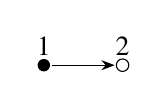
\begin{tikzpicture}
  \draw[-{Stealth}] (0.1,0) -- (0.9,0);
  \draw (0,0) node [above] {1};
  \draw (1,0) node [above] {2};
  \filldraw[fill=white] (1,0) circle (0.5ex);
  \fill[black] (0,0) circle (0.5ex);
\end{tikzpicture}.


$a_{21} \neq 0$,
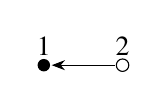
\begin{tikzpicture}
  \draw[-{Stealth}] (0.9,0) -- (0.1,0);
  \draw (0,0) node [above] {1};
  \draw (1,0) node [above] {2};
  \filldraw[fill=white] (1,0) circle (0.5ex);
  \fill[black] (0,0) circle (0.5ex);
\end{tikzpicture}.

$a_{12} \neq 0$, $a_{21} \neq 0$,
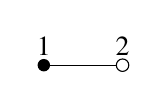
\begin{tikzpicture}
  \draw[-] (1,0) -- (0,0);
  \draw (0,0) node [above] {1};
  \draw (1,0) node [above] {2};
  \filldraw[fill=white] (1,0) circle (0.5ex);
  \fill[black] (0,0) circle (0.5ex);
\end{tikzpicture}.

������Ⱥϵͳ��, �����ǿ�Լϵͳ (ͼ����ͨ):
\begin{center}
  \begin{tikzpicture}
    \fill[black] (0,0) circle (0.5ex);
    \fill[black] (1,-1.7320508075689) circle (0.5ex);
    \fill[black] (2,0) circle (0.5ex);
    \draw[-] (0,0) -- (1,-1.7320508075689);
  \end{tikzpicture}
\end{center}
��ô��ֻ�������ֲ���Լ���:
\begin{center}
  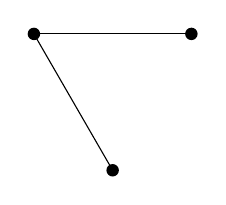
\begin{tikzpicture}
    \fill[black] (0,0) circle (0.5ex);
    \fill[black] (1,-1.7320508075689) circle (0.5ex);
    \fill[black] (2,0) circle (0.5ex);
    \draw[-] (0,0) -- (1,-1.7320508075689);
    \draw[-] (0,0) -- (2,0);
  \end{tikzpicture}
  \qquad
  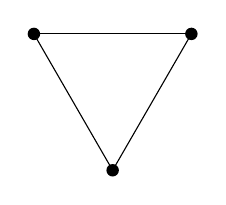
\begin{tikzpicture}
    \fill[black] (0,0) circle (0.5ex);
    \fill[black] (1,-1.7320508075689) circle (0.5ex);
    \fill[black] (2,0) circle (0.5ex);
    \draw[-] (0,0) -- (1,-1.7320508075689);
    \draw[-] (0,0) -- (2,0);
    \draw[-] (2,0) -- (1,-1.7320508075689);
  \end{tikzpicture}
\end{center}

�ܽ�:
\begin{center}
  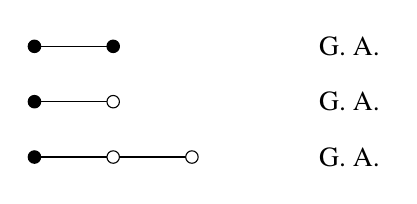
\begin{tikzpicture}
    \begin{scope}
      \draw[-] (0,0) -- (1,0);
      \draw[fill] (0,0) circle (0.5ex);
      \draw[fill] (1,0) circle (0.5ex);
      \draw (4,0) node {G. A.};
    \end{scope}
    \begin{scope}[yshift=-2em]
      \draw[-] (0,0) -- (1,0);
      \draw[fill] (0,0) circle (0.5ex);
      \filldraw[fill=white] (1,0) circle (0.5ex);
      \draw (4,0) node {G. A.};
    \end{scope}
    \begin{scope}[yshift=-4em]
      \draw[-] (0,0) -- (1,0);
      \draw[-] (1,0) -- (2,0);
      \draw[fill] (0,0) circle (0.5ex);
      \filldraw[fill=white] (1,0) circle (0.5ex);
      \filldraw[fill=white] (2,0) circle (0.5ex);
      \draw (4,0) node {G. A.};
    \end{scope}
  \end{tikzpicture}
\end{center}

��ϰ:
\begin{center}
\tikz \draw[fill] (0,0) circle (0.5ex) -- (1,0) circle (0.5ex) -- (2,0) circle (0.5ex) (4,0) node {G.A.?};
\end{center}

����:
\begin{center}
  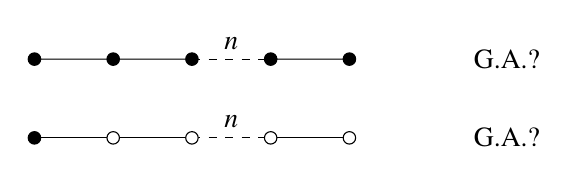
\begin{tikzpicture}
    \draw[fill] (0,0) circle (0.5ex) -- (1,0) circle (0.5ex) -- (2,0) circle (0.5ex);
    \draw[dashed] (2,0)  -- node [above] {$n$} (3,0);
    \draw[fill] (3,0) circle (0.5ex) -- (4,0) circle (0.5ex) (6,0) node {G.A.?};
    \draw (0,-1) -- (1,-1) -- (2,-1) (3,-1) -- (4,-1);
    \draw[dashed] (2,-1)  -- node [above] {$n$} (3,-1);
    \filldraw[fill=black] (0,-1) circle (0.5ex);
    \filldraw[fill=white] (1,-1) circle (0.5ex) (2,-1) circle (0.5ex) (3,-1) circle (0.5ex) (4,-1) circle (0.5ex) (6,-1) node {G.A.?};
  \end{tikzpicture}
\end{center}
������ֱ��� 1979��1981 ��֤������.
\begin{center}
  \begin{tikzpicture}
    \draw (0,0) -- (4,0);
    \draw[fill] (2,0) circle (0.5ex);
    \filldraw[fill=white] (0,0) circle (0.5ex) (1,0) circle (0.5ex) (3,0) circle (0.5ex) (4,0) circle (0.5ex) (6,0) node [right] {��ȫ���ȶ�.};
    \draw[dashed] (0,-1)  -- node [above] {$n$} (2,-1);
    \filldraw[fill=black] (1,-1) circle (0.5ex);
    \filldraw[fill=white] (0,-1) circle (0.5ex) (2,-1) circle (0.5ex);
    \draw (6,-1) node [right] {ֻҪ�кڵ�, $n \leq 4$, ȫ���ȶ�.};
  \end{tikzpicture}
\end{center}

һ���, ͼ��һ���� (��Ȧ):
\begin{center}
  \begin{tikzpicture}
    \draw (0,0) -- (1,0) (0,0) -- (-1,0) (0,0) -- (0,-1);
    \filldraw[fill=white] (-1,0) circle (0.5ex) (0,0) circle (0.5ex) (1,0) circle (0.5ex);
    \filldraw[fill=black] (0,-1) circle (0.5ex);
  \end{tikzpicture}
\end{center}
Color Test ����ͨ����������:
\begin{enumerate}[(1)]
  \item \tikz \draw (1ex,1ex) circle (0.5ex); ������;
  \item \tikz \fill[black] (1ex,1ex) circle (0.5ex); ����һ���׵�, ����һ���׵�.
\end{enumerate}
����ͨ�� Color Test, ��ȫ���ȶ�.

\chapter{ƽ��ϵͳ��֧}

\section{Hopf ��֧}

\begin{equation}\label{Eq:5.1}
\begin{aligned}
  \dot{x} & = \lambda x - y \underline{{} - a x y - y^2} = P(x, y),\\
  \dot{y} & = \lambda y + x \underline{{} + a x^2} = Q(x, y).
\end{aligned}
\end{equation}
���� $\underline{\qquad}$ ��ʾ��������.

����ϵͳ \eqref{Eq:5.1}, �� $\lambda < 0$ ʱ, ϵͳ����ȶ� (����), �� $\lambda > 0$  ʱ, ϵͳ��㲻�ȶ� (����), ����ΪϵͳΪ���Ľ�����.

$\lambda = 0$ ʱ, ����ֵʵ��Ϊ $0$, ��ʱ, ���� $V$ ����: $V =  (x^2 + y^2) + (x, y, 3) + (x, y, 4) + \cdots$, $(x, y, 3)$ �� $4$ ϵ��, $(x, y, 4)$  �� $5$ ϵ��. �� $\dot{V} = L(1) (x^2 + y^2)^2$, ��ͨ���ж� $L(1)$ �� $0$ �Ĵ�Сȷ������ȶ���. �� $L(1) = 0$, ���� $V =  (x^2 + y^2) + (x, y, 3) + (x, y, 4) + (x, y, 5)+ \cdots$ �õ� $\dot{V} = L(2)(x^2 + y^2)^3$.

ϵͳ \eqref{Eq:5.1} �� $L(1) = \frac{a}{4}$, �� $a < 0$, �����Ϊһ���ȶ�ϸ����, �� $a > 0$, �����Ϊһ�ײ��ȶ�ϸ����.

\begin{Exa}
  \begin{equation}
    \begin{aligned}
      \dot{x} & = - y - x (x^2 + y^2 - \lambda),\\
      \dot{y} & = x - y (x^2 + y^2 - \lambda).
    \end{aligned}
  \end{equation}
\end{Exa}
\begin{solve}
  ����ֵΪ: $\bar{\lambda} = \lambda \pm i$.
  \begin{enumerate}[(1)]
    \item $\lambda \neq 0 \Rightarrow$ �ֽ���, $\begin{matrix} \lambda > 0 & \text{���ȶ�} \\ \lambda < 0 & \text{�ȶ�} \end{matrix}$.
    \item $\lambda = 0 \Rightarrow$ ϸ���� (weak,  fine).
    
          $V = x^2 + y^2 \Rightarrow \dot{V} = - 2 (x^2 + y^2)^2 < 0 \Rightarrow$ ȫ���ȶ�ϸ����.
          
          ����: $\begin{matrix} \lambda > 0 & \text{���ȶ�} \\ \lambda \leq 0 & \text{�ȶ�} \end{matrix}$.
    \item $\lambda > 0$, �� $C = x^2 + y^2 - \lambda$.
          \begin{equation*}
            \dot{C}|_{c = 0} = 2 (x^2 + y^2) (\lambda - x^2 - y^2) = 2 (x^2 + y^2) \cdot C|_{c = 0} = 0
          \end{equation*}
          ����: ����һ�����ڽ� (���޻�, �Թ̶��� $\lambda$ ���ڽ����).
  \end{enumerate}
  ����:
  \begin{enumerate}
    \item $\lambda = 0$, �ȶ�; 
    \item $\lambda > 0$, ���ȶ�;  ($\lambda < 0$, �ȶ�).
  \end{enumerate}
  $\Rightarrow$ Hopf ���޻� (һ��ϸ�����֧).
\end{solve}

Hopf ��֧ ($\lambda = 0$, $a(0) = 0$, $b(0) > 0$).
\begin{equation}
  \begin{aligned}
    \dot{x} & = a(\lambda) x - b(\lambda) y + P_2(x, y, \lambda),\\
    \dot{y} & = b(\lambda) x + a(\lambda) y + Q_2(x, y, \lambda).
  \end{aligned}
\end{equation}
$O(0, 0)$ Ϊ���������, $P_2$, $Q_2$ �Ƕ������ϵĶ���ʽ.

\begin{Thm}\label{Th:5.1}\
  \begin{enumerate}
    \item $\lambda = 0$, $O(0, 0)$ �ȶ� (һ��ϸ����);
    \item $\lambda \neq 0$, $|\lambda|$ ���Сʱ $\Rightarrow$ ���ȶ�.
  \end{enumerate}
  �����Ψһ�ļ��޻�.
\end{Thm}
\begin{proof}
  \begin{enumerate}[(1)]
    \item ������ (ת������).
          \begin{equation*}
            \begin{aligned}
              \dot{\rho} & = a(\lambda) \rho + o(\text{�߽���}),\\
              \dot{\theta} & = b(\lambda) + o(\text{�߽���}).
            \end{aligned}
          \end{equation*}
          �� $b(0) > 0$ �ù�������ʱ���.
    \item $\lambda = 0$, ����ȶ�.
    \item $\lambda \neq 0$, $|\lambda|$ ���С,
          \begin{enumerate}
            \item ����������;
            \item ���ȶ�;
            \item ��ͼ \ref{Fi:5.1}, ���߹����˻���.
          \end{enumerate}
          $\Rightarrow$ (B-P), ���ڼ��޻�.
  \end{enumerate}
  \begin{figure}[!ht]
    \centering
    \subfloat[$\lambda = 0$.]{\includegraphics[width = 0.30\textwidth]{T5_1_a.eps}}
    \quad
    \subfloat[$\lambda \neq 0$.]{\includegraphics[width = 0.30\textwidth]{T90.eps}}
    \raisebox{2cm}{$\ \to \ $}
    \subfloat[���ɻ���.]{\includegraphics[width = 0.30\textwidth]{T91.eps}}
    \caption{���� \ref{Th:5.1}.}\label{Fi:5.1}
  \end{figure}
\end{proof}

\begin{Exa}
  \begin{equation*}
    \begin{aligned}
      \dot{x} & = \lambda x - y - a x y - y^2,\\
      \dot{y} & = x + \lambda y + a x^2.
    \end{aligned}
  \end{equation*}
\end{Exa}
\begin{solve}\ 
  \begin{enumerate}[(1)]
    \item $\lambda = 0$, һ�׽����� $L_1 = \frac{a}{4}$.
          \begin{equation*}
            \begin{aligned}
              V & = (x^2 + y^2) + (3) + (4),\\
              \dot{V} & = \frac{a}{4} (x^2 + y^2)^2 + o(V^2).
            \end{aligned}
          \end{equation*}
    \item $\bar{\lambda} = \lambda \pm i$.
          \begin{enumerate}[(i)]
            \item �� $\lambda = 0$, $a < 0$ �ȶ�; $\lambda > 0$, ���ȶ�. �ɶ��� \ref{Th:5.1} �õ����ڼ��޻�.
            \item $\lambda = 0$, $a > 0$, ���ȶ�; $\lambda < 0$, �ȶ�. �ɶ��� \ref{Th:5.1} �õ����ڼ��޻�.
          \end{enumerate}
  \end{enumerate}
\end{solve}

�� $\lambda = L(0)$, ��õ�:
\begin{Thm}[һ�� Hopf ����]
  $\lambda = L(0)$ �� $L(1)$ ���� $\Rightarrow \exists$ ���޻�. (����)
\end{Thm}

\section{���� Hopf}
���Ƕ���ϵͳ:
\begin{equation}
  \begin{aligned}
    \dot{x} & = \lambda x - y + l x^2 + m x y,\\
    \dot{y} & = x + x^2.
  \end{aligned}
\end{equation}
$O(0, 0)$ ���, $\lambda = 0$,
\begin{enumerate}
  \item $O$ Ϊϸ����. ($V = V(x, y) \Rightarrow \dot{V} = L(1) (x^2 + y^2)^2 + \cdots$), $L(1) = l(m - 2)$.
  \item \begin{equation*}
        l = 0\text{ (����) }
          \begin{cases}
            m \neq - 1, & B(x, y) = x^{\alpha} y^{\alpha}, \ \alpha = - \frac{m + 2}{m - 1},\\
            m = - 1,  & \dot{x} = - y (1 + x), \ \dot{y} = x (1 + x).
          \end{cases}
        \end{equation*}
  \item $l > 0$, $\begin{matrix} m > 2 & \text{���ȶ�} \\ m < 2 & \text{�ȶ�} \end{matrix}$ һ��ϸ����.
  \item $l > 0$, $m = 2 \Rightarrow L(1) = 0$. �� $V = V(x, y)$,
  
      $\Rightarrow \dot{V} = L(2) (x^2 + y^2)^3$, $L(2) = - 12 l$.
      
      \begin{equation*}
        \begin{matrix}
          L(0) = \lambda, & L(1) = l (m - 2), & L(2) = - 12 l,\\
          & (L(0) = 0 \Leftrightarrow \lambda = 0) & (L(0) = L(1) = 0 \Leftrightarrow \lambda = 0, \ m = 2)
        \end{matrix}
      \end{equation*}
      \begin{equation*}
        \dot{V} = l (m - 2) (x^2 + y^2)^2 + ( - 12 l) (x^2 + y^2)^3\  (m = 2 \ \text{ʱ}).
      \end{equation*}
\end{enumerate}

���� Hopf:
\begin{enumerate}
  \item $\lambda = 0$, $m = 2$. $L(2) = - 12 l < 0 \Rightarrow O$ ���ȶ���.
  \item $\lambda = 0$, $m > 2$, $m - 2 \ll 1 \Rightarrow O$ �Dz��ȶ��� $\Rightarrow$ ���ڼ��޻� ($L(1) \cdot L(2) < 0$).
  \item ȡ $|\lambda|$ ���С, �� $\lambda < 0 \Rightarrow$ ���ڼ��޻� ($L(1) \cdot L(2) < 0$).
\end{enumerate}
\begin{figure}[!ht]
  \centering
  \includegraphics{T92.eps}
  \caption{���� Hopf.}
\end{figure}

\section[Lyapunov ������˼��]{Lyapunov ������˼��\\ (����, ����, С�Ŷ����޻�) }

\begin{equation}\label{Eq:5.5}
  \begin{aligned}
    \dot{x} & = - y + \sum P_n(x, y),\\
    \dot{y} & = x + \sum Q_n(x, y).
  \end{aligned}
\end{equation}

Lyapunov ����:
\begin{equation}
  V(x, y) = x^2 + y^2 + \sum v_n(x, y).
\end{equation}
�������������㷨:
\begin{enumerate}
  \item ���Ǻ���,
  \item ��ʽ����,
  \item ������ʽ.
\end{enumerate}
�� \eqref{Eq:5.5} $V$ ���� $\dot{V}(x, y) = \sum \limits_{n = 1} L(n) (x^2 + y^2)^{n + 1}$, $L(n)$--$n$ �׽�����, \eqref{Eq:5.5}ϵ���Ķ���ʽ.

\begin{Thm}
  $\forall L(n) = 0 \Rightarrow O(0, 0)$ ������.
\end{Thm}

\begin{Thm}[Hilbert ��ԭ��]
  $\forall$ ����ʽ���� $\Rightarrow \exists$ �������ɻ�. ($f_ {\alpha} = \sum \limits^n_{i = 1} P_i f_i$.)
\end{Thm}

���� $L(1)$, $\dots$, $L(n)$, $\dots$, $\exists N > 0$ ʹ��, $L(1) = \cdots = L(N) = 0 \Rightarrow \forall n$,  $L(n) = 0$.

$L(1)$, $L(2)$, $L(3)$, $\dots$,
\begin{enumerate}[1)]
  \item �����ж��ȶ���,
  \item С�Ŷ����޻�, ѡ�����ʹ��,
        \begin{enumerate}
          \item $L(1) = \lambda = 0 \Rightarrow L(2) \cdot L(3) < 0$.
          \item $\lambda = 0 \Rightarrow L(1) \cdot L(2) < 0$.
          \item $\lambda \cdot L(1) < 0$.
        \end{enumerate}
        $\exists 3$ �����޻�.
\end{enumerate}

\begin{equation*}
  \begin{aligned}
    \dot{x} & = P_n(x, y),\\
    \dot{y} & = Q_n(x, y).
  \end{aligned}
\end{equation*}
$\hat{H}(n) = \max \{\text{С�Ŷ����޻�����}\}$, ���н���: $\hat{H}(2) = 3$, $\hat{H}(3) \geq 13$.


\backmatter

\end{document}
